\documentclass[
    paper=letter,
    12pt,
    titlepage,
    twoside,
    final,
    BCOR=10mm,
    DIV=9,
    listof=totoc]{scrbook}

\usepackage{fontspec}
\usepackage{microtype}
\usepackage[dvipsnames]{xcolor}
\usepackage{amsmath,amssymb,amstext,amsthm}
\usepackage{bm}
\usepackage{booktabs}
\usepackage{commath}
\usepackage[backend=biber,style=authoryear]{biblatex}
\usepackage{graphicx}
\usepackage{siunitx}
\usepackage{subcaption}
\usepackage{tikz}
\usepackage{unicode-math}
\usepackage{upgreek}

\usepackage[pagebackref=false]{hyperref}
\hypersetup{
    plainpages=false,       % needed if Roman numbers in frontpages
    unicode=false,          % non-Latin characters in Acrobat’s bookmarks
    pdftitle={An Integrated Model of Context, Short-Term, and Long-Term Memory},
    pdfauthor={Jan Gosmann},
%    pdfsubject={Subject},  % subject: CHANGE THIS TEXT! and uncomment this line
%    pdfkeywords={keyword1} {key2} {key3}, % list of keywords, and uncomment this line if desired
    pdfnewwindow=true,      % links in new window
    hidelinks,
}
\usepackage[capitalise]{cleveref}
\usepackage[automake,toc,nomain,nogroupskip,nonumberlist,nopostdot]{glossaries} % Exception to the rule of hyperref being the last add-on package
\usepackage{glossary-mcols}
\glssetwidest{$\mat M^{\ped{epis}}$}
\setglossarystyle{mcolalttree}


\usetikzlibrary{backgrounds}  % FIXME just for debugging
\usetikzlibrary{fit}
\usetikzlibrary{graphs}
\usetikzlibrary{nef}
\usetikzlibrary{positioning}
\usetikzlibrary{quotes}

\defaultfontfeatures[Lato]{
    UprightFont={Lato Regular},
    BoldFont={Lato Bold},
    Scale=MatchLowercase
}
\newfontfamily\lato{Lato}
\newfontfamily\lining{TeX Gyre Pagella}[Scale=MatchLowercase,Numbers=Lining]

\setmainfont{TeX Gyre Pagella}[Scale=MatchLowercase,Numbers=OldStyle]
\setmathfont{TeX Gyre Pagella Math}
\DeclareMathAlphabet{\mathcal}{OMS}{cmsy}{m}{n}
%\setmathfont{XITS Math}[range=cal]
\setsansfont{Lato}
\setkomafont{chapterentry}{\normalfont}
\sisetup{
    mode=math,number-math-rm=\lining,
    separate-uncertainty,
    multi-part-units=single,
}
\crefname{equation}{}{}
\Crefname{equation}{Equation}{Equations}

\renewcommand*{\partpagestyle}{empty}

\addbibresource{references.bib}
\addbibresource{proposal-references.bib}

\newcommand{\mat}[1]{\symbfit{#1}}
\newcommand{\vc}[1]{\symbfit{#1}}
\newcommand{\ped}[1]{{\mathrm{#1}}}
\newcommand{\Tr}{^{\top}}
\newcommand{\spc}[1]{\textsc{#1}}
\newcommand{\spv}[1]{\ensuremath{\mathbf{#1}}}

\allowdisplaybreaks
\DeclareMathOperator*{\argmax}{arg\,max}

\newcommand{\pop}[1]{{\lato #1}}  % chktex 1
\newcommand{\nin}[1]{{\lato #1}}  % chktex 1

\tikzset{net/.append style={font={\lato}},ext/.append style={font={\lato}}}

\newtheorem{defn}{Definition}
\newtheorem{corollary}{Corollary}
\newtheorem{lemma}{Lemma}

% Define Glossary terms (This is properly done here, in the preamble. Could be \input{} from a file...)

\newglossary*{symbols}{List of Symbols}
\makeglossaries

% List of Symbols
\newcommand{\addsym}[4]{\newglossaryentry{#2}{sort={#2},type=symbols,name={\ensuremath{#3}},description={#4}}\glsadd{#2}\newcommand{#1}{\ensuremath{#3}}}
\addsym{\tcmitem}{f}{\vc{f}}{TCM item vector}
\addsym{\tcmitemin}{fin}{\vc{f}^{\ped{IN}}}{recalled TCM item vector}
\addsym{\ctx}{c}{\vc{c}}{TCM context vector}
\addsym{\ctxin}{cin}{\vc{c}^\ped{IN}}{TCM input context vector}
\addsym{\mft}{Mfc}{\mat{M}^{\ped{FC}}}{TCM item to context matrix}
\addsym{\mtf}{Mcf}{\mat{M}^{\ped{CF}}}{TCM context to item matrix}
\addsym{\tcmbeta}{beta}{\beta}{TCM beta parameter}
\addsym{\Heavi}{heavi}{\Theta}{Heaviside function}
\addsym{\krond}{kronecker delta}{\updelta}{Kronecker delta}
\addsym{\enc}{e}{\vc{e}}{NEF encoding vector}
\addsym{\dec}{dec}{\vc{d}}{NEF decoding vector}
\addsym{\menc}{Enc}{\mat{E}}{NEF encoder matrix}
\addsym{\mdec}{D}{\mat{D}}{NEF decoder matrix}
\addsym{\weights}{W}{\mat{W}}{synaptic weight matrix}
\addsym{\act}{activity}{a}{neural spiking activity}
\addsym{\gain}{alpha}{\alpha}{NEF neuron gain}
\addsym{\jbias}{jbias}{J^{\mathrm{bias}}}{NEF bias input current}
\addsym{\nl}{G}{G}{neuron nonlinearity}
\addsym{\repspace}{Xc}{\mathcal{X}}{NEF representational space}
\addsym{\dims}{dim}{d}{dimensionality}
\addsym{\radius}{r}{r}{NEF representational radius}
\addsym{\syn}{h}{h}{synaptic filter}
\addsym{\syntau}{tausyn}{\tau_\ped{syn}}{synaptic time constant}
\addsym{\evalp}{x}{\vc{x}}{evaluation point}
\addsym{\actmat}{A}{\mat{A}}{activity matrix}
\addsym{\evalpmat}{X}{\mat{X}}{evaluation point matrix}
\addsym{\imat}{I}{\mat{I}}{identity matrix}
\addsym{\superpos}{S}{\mathcal{S}}{superposition operator}
\addsym{\simmeasure}{s}{s}{similarity measure}
\addsym{\bind}{B}{\mathcal{B}}{binding operator}
\addsym{\bid}{i}{\vc{i}}{identity under binding}
\addsym{\fourier}{F}{\mathcal{F}}{discrete Fourier transform}
\addsym{\fouriermat}{TF}{\mat{T}_{\mathcal{F}}}{discrete Fourier transform matrix}
\addsym{\bzero}{n}{\vc{n}}{absorbing element}
\addsym{\iu}{iu}{\symup{i}}{imaginary unit}
\addsym{\vtb}{BV}{\mathcal{B}_{\mathrm{V}}}{vector-derived transformation binding operator}
\addsym{\ndist}{N}{\mathcal{N}}{normal distribution}
\addsym{\expected}{Ex}{\symbb{E}}{expected value}
\addsym{\err}{Err}{E}{error}
\addsym{\errtotal}{Etot}{E_\ped{tot}}{total error}
\addsym{\errnoise}{En}{E_\ped{n}}{noise error}
\addsym{\errdist}{Ed}{E_\ped{d}}{distortion error}
\addsym{\bO}{O}{O}{big O notation}
\addsym{\sa}{Omega}{\Omega}{solid angle}
\addsym{\gammafn}{Gamma}{\Gamma}{gamma function}
\addsym{\betafn}{Beta}{\symup{B}}{beta function}
\addsym{\ballvol}{V}{V_{\!d}}{volume $d$-dimensional hyperball}
\addsym{\csdist}{CS}{\mathcal{CS}}{PDF of cosine similarity}
\addsym{\pcs}{pCS}{p_{\csdist}}{cosine similarity distribution pdf}
\addsym{\osestm}{mstm}{\vc{m^{\ped{stm}}}}{OSE short-term memory trace}
    \addsym{\oseepis}{mepis}{\vc{m^{\ped{epis}}}}{OSE episodic memory trace}
\addsym{\osestmdecay}{gamma}{\gamma}{OSE short term decay}
\addsym{\oseepisscale}{rho}{\rho}{OSE episodic scaling}
\addsym{\tauref}{tauref}{\tau_{\ped{ref}}}{refractory period}
\addsym{\taurc}{taurc}{\tau_{RC}}{membrane time constant}
\addsym{\drate}{phi}{\phi}{distractor rate}
\addsym{\reg}{lambda}{\lambda}{regularization scale}
\addsym{\posnum}{natural numbers}{\mathbb{N}_{>0}}{positive (excluding zero) natural numbers}
\addsym{\minev}{mu}{\mu}{null choice bias in recall}
\addsym{\recnoise}{sigma}{\sigma}{standard deviation of noise in recall}


%\includeonly{discussion}
\begin{document}

\pagenumbering{roman}

% The contents of the title page are specified in the "titlepage"
% environment.
\begin{titlepage}
        \begin{center}
        \vspace*{1.0cm}

        \Huge
        {\textsc{An Integrated Model of Context, Short-Term, and Long-Term Memory}}

        \vspace*{1.0cm}

        \normalsize
        by \\

        \vspace*{1.0cm}

        \Large
        Jan Gosmann \\

        \vspace*{3.0cm}

        \normalsize
        A thesis \\
        presented to the University of Waterloo \\ 
        in fulfillment of the \\
        thesis requirement for the degree of \\
        Doctor of Philosophy \\
        in \\
        Systems Design Engineering \\

        \vspace*{2.0cm}

        Waterloo, Ontario, Canada, 2018 \\

        \vspace*{1.0cm}

        \copyright\ Jan Gosmann 2018 \\
        \end{center}
\end{titlepage}

% The rest of the front pages should contain no headers and be numbered using Roman numerals starting with `ii'
\pagestyle{plain}
\setcounter{page}{2}

\cleardoublepage % Ends the current page and causes all figures and tables that have so far appeared in the input to be printed.
% In a two-sided printing style, it also makes the next page a right-hand (odd-numbered) page, producing a blank page if necessary.
 


% D E C L A R A T I O N   P A G E
% -------------------------------
  % The following is a sample Delaration Page as provided by the GSO
  % December 13th, 2006.  It is designed for an electronic thesis.
  \noindent
  This thesis consists of material all of which I authored or co-authored: see Statement of Contributions included in the thesis.
  This is a true copy of the thesis, including any required final revisions, as accepted by my examiners.

  \bigskip
  
  \noindent
I understand that my thesis may be made electronically available to the public.

\cleardoublepage

\begin{center}\textsc{Statement of Contributions}\end{center}
\Cref{sec:recall} (excluding \cref{sec:recall-net}) paraphrases a conference submission that was co-authored by myself, a PhD student Aaron R.\ Voelker, and my supervisor, Dr.\ Chris Eliasmith \parencite{jangosmann2017}.
\Cref{sec:apdx-wta} is a verbatim copy from the supplementary material accompanying the same paper.
I implemented the network models, performed the benchmarks, and data analysis.
Mr.~Voelker contributed the mathematical analyses.

A summary of \cref{prt:cue} of this thesis, co-authored by myself and my supervisor Dr.\ Chris Eliasmith, has been submitted to the CogSci 2018 conference \parencite{gosmann2018}.

\cleardoublepage

% A B S T R A C T
% ---------------

\begin{center}\textsc{Abstract}\end{center}
I present the context-unified encoding (CUE) model, a large-scale spiking neural network model of human memory.
It combines and integrates activity-based short-term memory with weight-based long-term memory.
The implementation with spiking neurons ensures biological plausibility and allows for predicitions on the neural level.
At the same time, the model produces behavioural outputs that have been matched to human data from serial and free recall experiments.
In particular, well known results such as primacy, recency, transposition error gradients, and forward recall bias have been reproduced with good quantitative matches.
Additionally, the model accounts for the effect of the acetylcholine antagonist scopolamine.

To construct the CUE model, the Neural Enineering Framework (NEF) and Semantic Pointer Architecture (SPA) have been utilized.
This thesis makes novel contributions to both.
I propose to distribute NEF intercepts according to the distribution of cosine similarities of random uniformly distributed unit vectors.
This leads to a uniform distribution of active neurons and reduces the error introduced by spiking noise considerably in high-dimensional neuronal representations.
It improves the asymptotic scaling of the noise error with dimensions $\dims$ from $\bO(\dims)$ to $\bO\big(\dims^{3/4}\big)$.
These results are applied to achieve improved Semantic Pointer representations in neural networks which are on par or better compared to previous methods of optimizing neural representations for the Semantic Pointer architecture.
Furthermore, the vector-derived transformation binding (VTB) is investigated as an alternative to circular convolution in the SPA with promising results.

The CUE model combines and extends the ordinal serial encoding (OSE) model, a spiking neuron model of short-term memory, and the temporal context model (TCM), a mathematical model of free recall.
To the former a neural mechanism for tracking the list position is added.
The latter is converted into a spiking neural network under considerations of the main features and simplifying equations where appropriate.
Previous models of the recall process in the TCM are replaced by a new independent accumulator recall process that is more suited to the integration in a large-scale network.
To implement the modification of the required association matrices, a novel learning rule, the association matrix learning rule (AML), is derived that allows for one-shot learning without catastrophic forgetting.
Its biological plausibility is discussed and it is shown that it accounts for changes in neural firing observed in human recordings from an association learning experiment.
Furthermore, I discuss a recent proposal of an optimal fuzzy temporal memory as replacement for the TCM context signal and show it to be likely to require more neurons than the human brain consits of.


\cleardoublepage

% A C K N O W L E D G E M E N T S
% -------------------------------

\begin{center}\textsc{Acknowledgements}\end{center}
I would like to thank my supervisor, Chris Eliasmith, for his continued support and guidance.
I am also grateful to my colleagues at the Centre for Theoretical Neuroscience, in particular Terrance Stewart and Aaron Voelker, for their invaluable knowledge and helpful discussions.
The research in this thesis would have not been possible without the excellent and continuously improving work of the Nengo development team, spearheaded by Trevor Bekolay.
This research was also enabled in part by support provided by SHARCNET\footnote{\href{https://www.sharcnet.ca}{www.sharcnet.ca}} and Compute Canada\footnote{\href{https://www.computecanada.ca}{www.computecanada.ca}}.
Many CPU cycles were burned on their hardware simulating iterations of the CUE model.
I also would like to acknowledge the financial support for this research by the Canada Research Chairs program, the NSERC Discovery garnt 261453, the Air Force Office of Scientific Research grant FA8655-13-1-3084, CFI, and OIT\@.  % chktex 8

A special mention is deserved by the Interdisciplinary College, a unique annual spring-school at the Lake Möhne in Germany.
It is the place where I met Chris Eliasmith for the first time and ultimately made me pursue this research direction.

Finally, I would like to thank all the people I climbed with over the years as they helped me to stay sane during this period.


\cleardoublepage

% D E D I C A T I O N
% -------------------

\begin{center}\textsc{Dedication}\end{center}

This is dedicated to the one I love. TODO
\cleardoublepage

% T A B L E   O F   C O N T E N T S
% ---------------------------------
\renewcommand\contentsname{Table of Contents}
\tableofcontents
\cleardoublepage

% L I S T   O F   T A B L E S
% ---------------------------
\listoftables
\cleardoublepage

% L I S T   O F   F I G U R E S
% -----------------------------
\listoffigures
\cleardoublepage

% GLOSSARIES (Lists of definitions, abbreviations, symbols, etc. provided by the glossaries-extra package)
% -----------------------------
\printglossaries
\cleardoublepage

\pagestyle{headings}
% Change page numbering back to Arabic numerals
\pagenumbering{arabic}
 
\chapter{Introduction}

Memory in its different forms is an important aspect of human, but also animal cognition.
For example, it allows animals to return to previously visited water and food locations (TODO refs).
Prior experiences also allow to act more optimally in similar situations or avoid dangerous situations.
In this sense memory allows for adaptation on a faster time scale than genetic selection.
This is especially important in unstable and changing environments.
In humans, memory is also important to form social relationships, a shared culture, and even a functioning society.
Moreover, it contributes to our individual sense of self.
In general, the storage of information over time is a fundamental requirement in many cognitive systems and also from a computational point of view an addressable memory is important as it allows for more compact implementations than a pure state machine (TODO cite Gallistel).

Accordingly, there is a long history of memory research.
The well-known primacy and recency effect (discussed in more detail in TODO) have already been described by TODO Robinson, Brown 1926.
Nevertheless, there are still many open questions.
One important challenge that has to be solved by a memory system is the so-called \emph{stability-plasticity dilemma} (TODO ref Abaraham and A Robins 2005).
On the one hand, there is a need to quickly form new memories, sometimes even with a single exposure known as \emph{one-shot learning}.
On the other hand, such high plasticity can easily lead to overwriting of old memories rendering memory system useless.
TODO refo Buzsaki and others proposed multi-stage memory models where different memory system are in place for different timescales with different levels of plasticity.
However, this still leaves open TODO questions.

It also is a strong indication that different memory systems interact.
Though, it much of experimental research and modeling different memory systems have been treated as isolated.
This simplifies the analysis on a certain level, but to get a general understanding of memory as a whole the results need to integrated at some point.
Furthermore, many models of memory or learning focus on either small scale neural changes without any direct connection to behaviour or on the other extreme of describing behaviour with mathematical equations, but no solid grounding in biological plausibility.
So it is not only important to integrate our understanding of memory systems, but also to bridge the gap from neural mechanisms to behaviour.
This thesis will try to advance our understanding in this direction.

While this will still be comparably rough sketch and still fairly limited in memory systems covered, there are promising long-term prospects from a better understanding of human memory.
Many forms of memory loss are currently untreatable.
However, diseases associated with aging like Alzheimer's significantly impair the function of memory and are getting more common as our life-span increases due to other medical and nutritional advances.
(TODO stroke, hippocampal lesions?)
A better understanding of memory might allow us to devise better treatments or even stop and reverse the memory detoriation.
A potential route to this are memory implants that have already been demonstrated in rats by TODO Berger et all 2011.
For this sort of implant, an understanding of how memories are encoded is at least helpful if not crucial.

These are certainly strong motivators for research into memory, but it is also worthwhile to advance our general understanding of how the human brain works.
A question that has puzzled researchers for a long time and probably still will for a long time to come despite great advances.
An important step in testing our current understanding of the brain was the Spaun model (TODO ref).
A spiking neural network of XX neurons, thus grounded in biology, that can perform 8 different tasks.
Like a real brain it gets sensory input (low resolution black and white symbols) and produces a behavioural motor output with a simulated arm.
The number of tasks it can perform demonstrates that it is not a specialized model for a single task, but can switch between different tasks like a real brain.
Obviously, Spaun is still much simpler (and has much less neurons) like a real brain.
So there is no denying that it is still a long way to a full understanding of the whole brain.
But it incorporates a number of qualitative key aspects.
However, one key aspect is still missing.
While it can perform working memory dependent tasks and has simple reinforcement learning, it is missing a declarative and episodic long-term memory.
The work in this thesis is also a step towards providing Spaun with such a memory by integrating it with a short-term memory component similar to the one used in Spaun.


\section{Behavioural characterization of memory}
Memory is commonly characterized along two orthogonal dimensions:
by timescale and by type of information stored.
On the timescale axis one usually discriminates between short-term memory (STM), and long-term memory or short-term, long-term, and very long-term memory (vLTM).
However, there is no single agreed upon definition which timescales are encompassed in each of these terms.
Sometimes LTM is used to refer to vLTM, while sometimes LTM is in-between STM and vLTM\@.
As a rough orientation STM is usually taken to be on the sub-second timescale, up to a few seconds.
Very long-term memory is on timescales of weeks and up (TODO verify).
LTM, depending on the definition, covers timescales from minutes and up.
Moreover, the term working memory (WM) is often used to refer to active representations that allow direct mental manipulation.

In this thesis, I will use the term STM for timescales in the order of seconds and LTM for longer timescales, but separate from vLTM\@.
Moreover, I will assume STM to be based on neural-activity and thus this definition is somewhat in line with the definition of WM\@.

When classifying memory by type of information, a representation as a tree structure can be helpful.
On the highest level, we have the distinction between implicit and explicit memory.
Implicit memory does not allow for conscious access.
A typical example is procedural or motor memory like how to ride a bike.
Explicit memory allows for conscious access and is further subdivided into declarative and episodic memory.
The declarative memory allows us to store and reproduce facts like the birthday of a friend, whereas the episodic memory provides a recollection of life experiences.

Here, I will focus on declarative memory as this type of memory has been well studied in many memory experiments.


\section{Experimental findings in memory research}
Most memory experiments require the participants to memorize lists of words and recall them afterwards.
The words are typically chosen from the Toronto noun pool and are matched for semantic similarity and occurrence frequency (TODO verify, ref).
Usually an experiment will fall in one of two categories depending on how the subjects are required to recall the list items: in free recall experiments, the subjects are free to recall the items in any order; in serial recall experiments, the subjects are required to recall the items in order.

The hallmark finding in memory research, especially for serial recall experiments, are the primacy and recency effect.
Subjects tend to remember the start of list (primacy) and the end of list (recency) better (TODO fig).
Furthermore, if subjects in a serial recall experiment recall an item at the wrong position, a so-called \emph{transposition}, it is more likely to be an item that was close in the list than an item several positions spaced out.

In free recall experiments, participants usually start out by recalling the last items first.
This can be measured by the probability of first recall (TODO fig).
There is also the tendency, to recall items in forward direction and items close to the last recalled item.
The conditional response probability (CRP) measures this (TODO fig)
It gives the probability of how many items forward or backward (know as the lag) the next recall will jump.

In memory experiments the recall phase can directly follow the study phase, known as an immediate recall experiment, or a delay, potentially with a distractor task, can separate the two, known as delayed recall.
Sometimes a distraction task will be performed in between each list item which is known as continuous distractor recall.


\section{Neuroanatomy of memory}
TODO brain regions involved in short term recall

The hippocampus (HC) has been implicated in the acquisition of new episodic memories.
A finding derived from patients with hippocampal lesions, most famously HM who got his hippocampus removed due to severe epilepsy (TODO refs).
The hippocampus is named for his sea horse shaped structure.
It is located in the medial temporal lobe (TODO fig) and neighbours the subiculum and entorhinal cortex (EC).
The hippocampus is further divided into substructures CA3, CA1, and the dentate gyrus (DG) by its cytoarchitectural structure.
While the CA3 and CA1 regions consist mainly out of pyramidal neurons and about \SI{10}{\percent} GABAergic, inhibitory interneurons (TODO ref Freund and Buzsaki 1996), granule cells are the main constituent of the dentate gyrus.
Furthermore, the dentate gyrus has a large number of cells compared to CA3.
In humans the cell count of the DG is about twice as high as in CA3, whereas in rats DG has about five times more cells than the CA3 region.

The connectivity to, from, and within hippocampus is exceptionally well known.
There are two major pathways from entorhinal cortex.
The direct pathway originates in layer III of the entorhinal cortex and targets the distal apical dendrites of CA1 neurons.
The trisynaptic pathway originates in layer II and leads via the dentate gyrus, and CA3 also to CA1, but targeting the proximal dendrites (a signal thus crosses three synapses).
The connections from the dentate gyrus to the CA3 region in this is termed the mossy fiber pathway.
Each of these mossy fibers innervates about 15 neurons (TODO ref Claiborne, Amaral and Cowan 1986) which results in each CA3 pyramidal neuron receiving input from about 50 to 90 granule cells (TODO ref Squire, Shimamura, and Amaral 1989, p230).
The final bundle of connections from CA3 to CA1 is known as the Schaffer collateral pathway.

TODO further connections: EC to CA3 (mostly targeting same cells as from DG, Paxinos 2014), CA3 recurrent (single cell not innervated by more than 5\% of all CA3 cells Squire, Shimamura and Amaral 1989, p231)

Given these neuroanatomical properties, some of the hippocampal regions have been assumed to be involved in specific tasks.
The sparse cdoing and large cell count of the dentate gyrus led to the belief that it is responsible for pattern separation (TODO ref Rolls 2013).
The CA3 region with its recurrent connectivity could be involved in pattern completion or forward predictions (TODO ref Leutgeb and Leutgeb 2007, Rolls 2013).
Additional evidence for this comes from context dependent firing of these neurons (TODO how so? TODO ref Guzowski, KHierim, and Moser 2004, Leutgeb and Leutgeb 2007) and unimpaired recognition memory after lesioning the CA3 to CA1 connections despite impairing selective recall (TODO ref Brun et al 2002). 

theta rhythm, SPWs, grid and place cells

vLTM not hippocampal
Cerebellum for motor


\section{Memory models}
TODO discuss desired properties of models
TODO categorization by conceptual, abstract mathematical, and neural models

\subsection{Conceptual models}
\Textcite{Yntema1963} presented one of the first models of memory.
They conceptualized retrieval as a search process where each item in memory is associated with tags referencing further information.
For example, a time tag would encode the time an item was observed.
The whole description, however, is more based on how a memory system could be implemented on a classical von Neumann computer and does not consider if or how those operations could be neurally implemented.

To date, the most influential conceptual organization of working memory was proposed by \textcite{Baddeley1986}.
He proposed, based on experimental data, separate stores for visual and acoustic information, termed the visuospatial sketchpad and phonological loop respectively.
These are controlled by a central executive.
Furthermore, in \textcite{Baddeley2000} the model was extended with an episodic buffer for the binding of multimodal information and transfer to episodic long-term memory.
The main relevance of the model is that it informs us about the organization of (working) memory by modality; but it does less to elucidate mechanisms.

In general, conceptual models can give a high-level account and they can be evaluated with respect to their qualitative agreement to behavioural data.
However, they cannot provide us with quantitative predictions which makes a more rigorous validation difficult.
They also, do not explain the cognitive mechanisms in detail and an account of the neural implementation is completely out of their reach.


\subsection{Mathematical models}
Some of the weaknesses of conceptual models are addressed by mathematical models.
These models will make quantitative predictions about the behavioural data and describe underlying cognitive mechanisms to a varying degree, but do not provide a neural implementation.
There is a vast amount of such models and not all can be discussed here.
Thus I will focus on the most influential ones.

That list certainly contains the perturbation model for serial order by \textcite{Estes1972}, the free recall model Search of Associative Memory (SAM) by \textcite{Raaijmakers1981}, the recognition memory model Retrieving Effectively from Memory (REM) by \textcite{Shiffrin1997}, and the episodic memory model MINERVA2 by \textcite{Hintzman1988}.
The perturbation model an early attempt to provide a mathematical framework of how remembered item positions can drift over time.
In SAM cues are assembled in a short-term memory to retrieve associations from a long-term associative memory (the search part of the model).
In the REM model error prone copies of feature vectors derived from the study items are stored.
A recognition probe is matched to the stored feature vectors and a likelihood ratio of the match scores being generated by an old vs.\ a new item is calculated.
The MINERVA2 model also uses feature vectors that are stored as traces and can be probed by cues.

All of these models, and most other mathematical model, either assume item-to-item or position-to-item associations.
The primacy model by \textcite{Page1998} is worth noting because it uses a different approach.
In that model items are activated according to a primacy gradient, but the model is agnostic to how this gradient is generated.
This, however, also leaves that aspect underspecified.

Common to all of these models is that they are not demonstrating biological plausibility.
Thus it is unclear, whether any of the models can be implemented in a neural substrate while preserving the predictions.
Or even if, what the limitations with regard to noise and requirements for neural resources are.
Nevertheless, mathematical modelling is an important first step in figuring out what sort of processes are worth considering for a neural implementation.
Also, there are some reoccurring ideas in these models that are useful to consider in the context of a neural model.
For example, starting with \textcite{Anderson1973} many models have used random feature vectors to represent individual items.
That approach is similar to the Semantic Pointer Architecture (SPA) presented in Section TODO which can be implemented neurally with the methods of the Neural Engineering Framework (NEF, Section TODO).

An especially influential model based and random feature vectors was TODAM2 \parencite{Murdock1993}.
It was able to fit a large body of experimental data and in that aims to be a general theory for item recognition, serial order, and associative memory.
A neural implementation could very well be possible with the NEF, but has not been attempted so far.
However, \textcite{Choo2010} pointed out that the dimensionality of the vectors in the model increases with each stored item.
Thus, the requirement for neural resources grows unbounded.
It also worth noting, that TODAM2 does not give an account of how responses are generated.

Another useful idea, that had its origin in mathematical models, is the idea of a randomly drifting context signal that items get associated to.
\Textcite{Estes1955} presented the first model of this type and \textcite{Murdock1997} extended the TODAM2 model in this way to explain additional data.
An open question in these sort of models is, how the context at an earlier time can be re-instantiated to start the recall and how the context is advanced in the same way during recall as in the study phase to recall the remaining items.
As the signal drifts randomly a memory for the context signal itself would be needed.
The OSCAR model \parencite{Brown2000} solves part of this by using a deterministic context signal that is generated from multidimensional oscillators.
This allows to replay the exact same context signal once it has been reset.
It still does not answer how the context is re-instantiated to start the recall as this still requires knowledge of the oscillator states at begin of the study phase.

All of these context-based models cannot explain the asymmetric CRP curves.
The temporal context model (TCM, TODO ref), however, was specifically constructed to explain these free recall data.
It also uses a context signal, but this signal is updated by the studied (and recalled) items themself.
Each item recalls a prior context associated with that item to partially update the current context and the updated context gets associated with the studied item.
This solves the re-instantiation problem as the right cue can set the context to be similar to the study context to retrieve an item.
That retrieved item in turn updates the context to retrieve more items related to the updated context.
Thus, it is also available to appropriately advance the context after each recall.
The model will discussed in more detail in TODO\@.
But the TCM is not perfect.
It did not capture immediate free recall data involving short-term memory, even though it was presented as a single-store framework, i.e.\ a single memory for both STM and LTM\@.
TODO Davellar 2008 critique (does CUE capture the data?)

Many of these models are also vague on the exact processes of recall.
The ACT-R model of serial recall by \textcite{Anderson1997}, in which items are associated with their serial positions, describes detailed steps necessary for recall.




\begin{itemize}
    \item fuzzy temporal memory
    \item Start-End Model (SEM) (Henson, 1998) reproduces relative positional coding within groups (probably only one), not clear how endmarker can be generated (despite suggestions in the paper)
    \item Anderson and Matessa 1997 ACT-R model of serial recall, items are associated with serial position and grouped. Detailed steps of recall, but no neural implementation or specification of how exactly items are stored.
\end{itemize}


Mention?
\begin{itemize}
    \item context-signal-based models: grouping structure has to be known in advance for grouping effects
\end{itemize}


\subsection{Connectionist models}
Compared to the vast amount of mathematical models, there are much fewer connectionist models that try to ensure more biological realism.
Many of these models focus on reproducing low-level findings in the hippocampus such as sequence compression in replay \parencite{Levy2005} or place cells \parencite{Milford2004}.
The model presented by \textcite{Hasselmo2012}, might very well be the most comprehensive hippocampus model to date describing the storage of episodic memories as a spatial trajectory.
It addresses experimental data on place cells and the theta rhythm (TODO explained?).
A very recent model TODO ref Yu, constructs a three-layer spiking neural network that is able to encode a sequence over several iterations and replay it during a cycle of the theta rhythm.
These models, however, still leave a large gap to high-level cognitive behaviour as modelled by mathematical models.
In addition, the \textcite{Hasselmo2012} relies on hypothetical ``arc length'' cells to disambiguate memories \parencite[cp.][]{Robins2014}.

Nevertheless, there are some connectionist models that try to reduce this gap by addressing behavioural effects with a neural network implementation.
Namely, \textcite{Burgess1992} and \textcite{Burgess1996} proposed models for the articulary loop, \textcite{Norman2003} for recognition and familiarity effects, and \textcite{Botvinick2006} for immediate serial recall.
All of these models use rate based neurons as an abstraction.
While these are a useful tool to build tractable biological plausible models, one has to be careful to not introduce biologically implausible features.
For example, the noise introduced by discrete spikes is neglected.
In particular, \textcite{Norman2003} use a $k$-winner-take-all mechanism that is hard to realize in spiking neurons as it requires a fine balance of excitation and inhibition.
Potentially even more problematic is the use of back-propagation learning and a softmax function applied to the network outputs in the model by \textcite{Botvinick2006}.
While learning with back-propagation is a tremendously successful technique in machine learning, it is still unclear whether biological neural networks can implement this sort of learning.
But see work on feedback-alignment TODO and talk in lab TODO\@.
The softmax function is problematic for biological plausibility as it requires global knowledge of the network outputs.
TODO why is this a problem?

I only know of two memory-related models that address the these concerns about biological plausibility by using spiking neurons while at the same time connecting to behavioural data.
The first one is the ordinal serial encoding (OSE) model of serial recall by \textcite{Choo2010}.
As a primarily short-term memory model, it uses recurrently connected neurons to store the memory trace in neural activity.
This approach is also used to model a long-term memory component that can be attributed to hippocampal storage.
While this allows for a first approximation, a storage in synaptic weights seems more realistic for such a component.
The second model was specifically developed to model the storage of serial lists with hippocampus by \textcite{OliverTrujillo2014}.
It is able to reproduce neural data like replay and theta rhythm.
However, the length of stored lists is limited in similar fashion as STM capacity while long term memory is certainly able to learn longer lists.
Learning longer lists in the model would require the chaining of individual lists with different contexts, but not mechanism for this has been given in the model.
Another questionable feature is the usage of a clock signal that is adjusted to speed up compressed replay.


\subsection{Summary}

CUE\@: neural implementation (biological plausibility), includes recall/reinstantiation of context, (limited neural resources)


Further points (some maybe for conclusion, not introduction?):
\begin{itemize}
    \item Large scale modeling has new challenges.
    \item How do things interact?
    \item How are they coordinated?
    \item Increases to simulation speed (better neural representation, optimizer)
\end{itemize}

\part{Methods}
\chapter{Modeling neurons}\label{sec:neurons}
The information processing in the brain is performed by neurons (see \cref{fig:neuron}).
Despite a wide variety of different neuron types and behaviours, the typical behavior of most neurons can be described as follows.
These cells build up an electrical potential of about \SI{-70}{\milli\volt}, the \emph{resting membrane potential}, across their cell membrane with the ions in the intra- and extracellular fluid.
When the membrane potential is sufficiently depolarized (to about \SI{-50}{\milli\volt}), voltage gated ion channels trigger a sudden and short-lived depolarization (typically about \SI{1}{\milli\second}), generating a so-called action potential or spike.
This action potential travels along the neuron's axon and triggers the release of neurotransmitters at the boutons, which open into synapses, where the axon comes extremely close to other neuron's dendrites.
The released neurotransmitters will influence the ion channels of the post-synaptic neuron and either lower (inhibitory synapse) or raise (excitatory synapse) the membrane potential.
The deflection of the membrane potential depends on the strength of the synapse and the speed of the release and uptake of the neurotransmitter.
If the post-synaptic neuron receives sufficient input from other neurons, its membrane potential will be sufficiently deflected to initiate a new action potential.
By the pattern of connectivity that controls what activity in some neurons triggers activity in other neurons, the brain is able to perform the computations that lead to an agent's behavior.

\begin{figure}
    \centering
    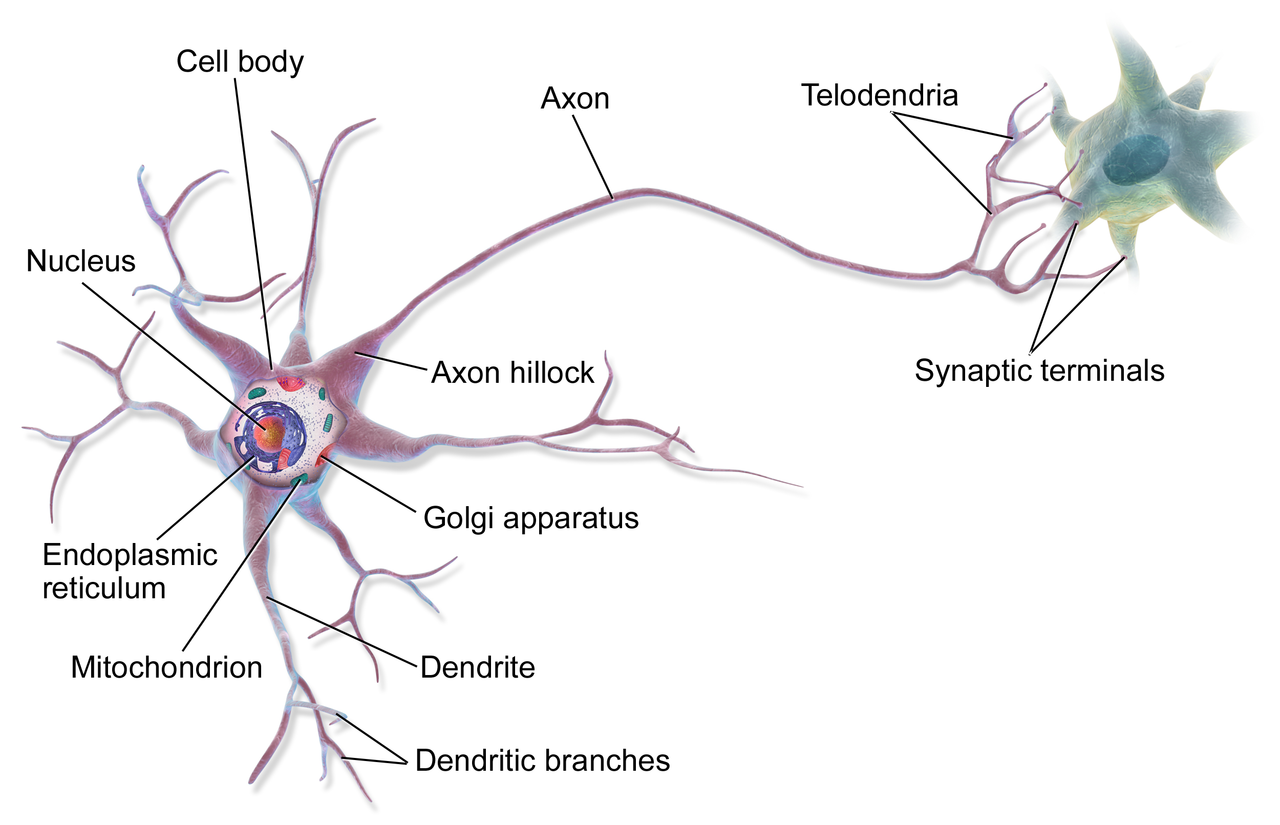
\includegraphics[width=0.8\textwidth]{figures/Blausen_0657_MultipolarNeuron}
    \caption[A typical neuron.]{A typical neuron. Image by Blausen Medical Communications, Inc.\ and reused under the Creative Commons Attribution 3.0 Unported license.}\label{fig:neuron}
\end{figure}

To model neurons computationally, it is necessary to chose a level of abstraction.
On the one hand, it is possible to create very detailed models with spatial extent \parencite[e.g.,][]{markram2015,bahl2012} where individual ion channels and the propagation of electrical potentials is modeled.
On the other hand, one can use very abstract neuron models that basically consist of nodes summing their inputs and applying non-linearity using real valued stand-ins for firing rates (instead of discrete spikes).
This latter type of model is common in artificial neural networks and deep learning.

A widely used neuron model in computational neuroscience, that is midway between these two extremes, is the leaky integrate-and-fire (LIF) neuron model.
It is a point neuron model, thus not modeling any spatial extend.
It models a single membrane voltage $V(t)$ described by the differential equation
\begin{equation}
    \taurc \od{V}{t} = -V(t) + R J(t)
\end{equation}
where $R$ is the membrane resistance, $J(t)$ the input current, and $\taurc$ the membrane time constant.
Whenever the membrane voltage reaches a certain threshold $V_{\!\ped{th}}$, the LIF neuron transmits a spike and its membrane voltage is reset for a refractory period of $\tauref$.
This type of neuron model allows the firing rate to be derived for a given constant input current $J$ as
\begin{equation}
    \act(J) = \frac{1}{\tauref - \taurc \ln\!\del{1 - \frac{V_{\!\ped{th}}}{R J}}} \text{.}
\end{equation}

The LIF neuron model is a good choice for the undertaking of this thesis as it captures many aspects of neuron behaviour.
It is detailed enough to relate parameters like the membrane time constant to the actual biological correspondents.
This allows us to fix these parameters to values within a biologically plausible range instead of having them as free parameters in the model that would require parameter matching and give the model additional degrees of freedom to match the data.
At the same time, the model is simple enough to allow for reasonable performance when simulating large-scale models with these neurons.

\chapter{The Neural Engineering Framework}\label{sec:nef}

To construct a large-scale spiking neural network with a certain behaviour, some method for obtaining that behaviour is required.
In most cases this method will be a learning algorithm \parencite[e.g.,][]{oreilly2006}.
However, this requires time-intensive training of the model and is often not viable for large models, complex behaviours, or models combining different behaviours.
In this work I opt to use the Neural Engineering Framework \parencite[NEF;][]{eliasmith2003} which allows the direct construction of a spiking neural network from the mathematical equations describing the desired dynamics without the time-intensive training.
As such the final model does not provide an developmental account of how the neural network became organized or learned to perform its task.
But, it provides a biologically plausible explanation of how the developed brain might perform that task.
As well, it allows for the inclusion of biologically plausible online learning rules, to test adaptation in the adult system.
Furthermore, it allows for manipulations to test known experimental results in the model or obtain new predictions.
The NEF consists out of the three core principles for \emph{representation}, \emph{transformation}, and \emph{dynamics} in a neural network that I introduce in this order.

\section{Representation}
Neurons within a neural network will have a preferred stimulus: they will fire most strongly for that stimulus and less strongly as the stimulus gets more dissimilar to the preferred stimulus (see \cref{fig:tuningcurve}).
To capture this in a mathematical description, we can treat the stimulus as a vector $\vc x(t)$ that varies over time.
The preferred stimulus vector, that is the vector a neuron $i$ fires most strongly for, will be denoted with $\enc_i$.
The spiking activity $\act_i(t)$ of a neuron can then be described with
\begin{equation}
    \act_i(t) = \nl\!\sbr{\gain_i \langle\enc_i, \vc x(t)\rangle + \jbias_i}
\end{equation}
where $\gain_i$ is a neuron gain factor, $\jbias_i$ a bias input current, and $\nl$ the neuron nonlinearity.
The nonlinearity $\nl$ represents the neuron model and converts an input current into spikes.
Usually this is the spiking, leaky integrate-and-fire model (LIF) discussed in \cref{sec:neurons}, which provides a good trade-off of captured neuron behaviour, detail, and simulation effort.
But simpler neuron models (e.g., a rate-based LIF model, or rectified linear units) could be used, as well as much more complex neuron models, like the compartmental models in \textcite{eliasmith2016} and \textcite{duggins2017c}.
The input current to the neuron is obtained from how well the stimulus aligns with the preferred stimulus as measured by the dot product.
As this alignment with the preferred stimulus ``encodes'' the stimulus into the neural representational space, $\enc_i$ is usually referred to as \emph{encoder} in the context of the NEF\@.
Furthermore, the gain factor $\gain_i$ and bias term $\jbias_i$ can be used to adjust the neuron's tuning curve to experimentally observed firing rates.
However, it is also common to use higher maximal firing rates to use fewer neurons in simulations while achieving an similar accuracy.
While this is not entirely adhering to biological constraints, in most cases NEF models behave similarly when lowering the firing rates and increasing neuron numbers accordingly \parencite[e.g.,][]{gosmann2015}.
As it is rare to have detailed information about the tuning curves in many parts of the brain, those values are usually not directly set in the NEF\@.
Instead a representational space $\repspace$ is defined, usually as the $\dims$-dimensional $\dims$-hyperball with radius $\radius$.
Furthermore, for each neuron a maximum firing rate $\act_{\max, i}$ and an intercept point $p_i$ are sampled from random distributions.
These values are used to calculate the gain and bias so that the neuron starts firing at $p_i \enc_i$ when $\vc x$ varies along the encoder $\enc_i$ and that the maximum $\act_{\max,i}$ is not exceeded across the representational space $\repspace$.
\begin{figure}
    \begin{captionbeside}[A typical neuron tuning curve.]{A typical neuron tuning curve. The thick black line shows the mean firing rate in dependence of a stimulus parameter (e.g., rotation of a bar). The thin blue lines show the standard deviation. Figure reproduced from \textcite{butts2006} and reused under the Creative Commons Attribution license.\label{fig:tuningcurve}}[l]
        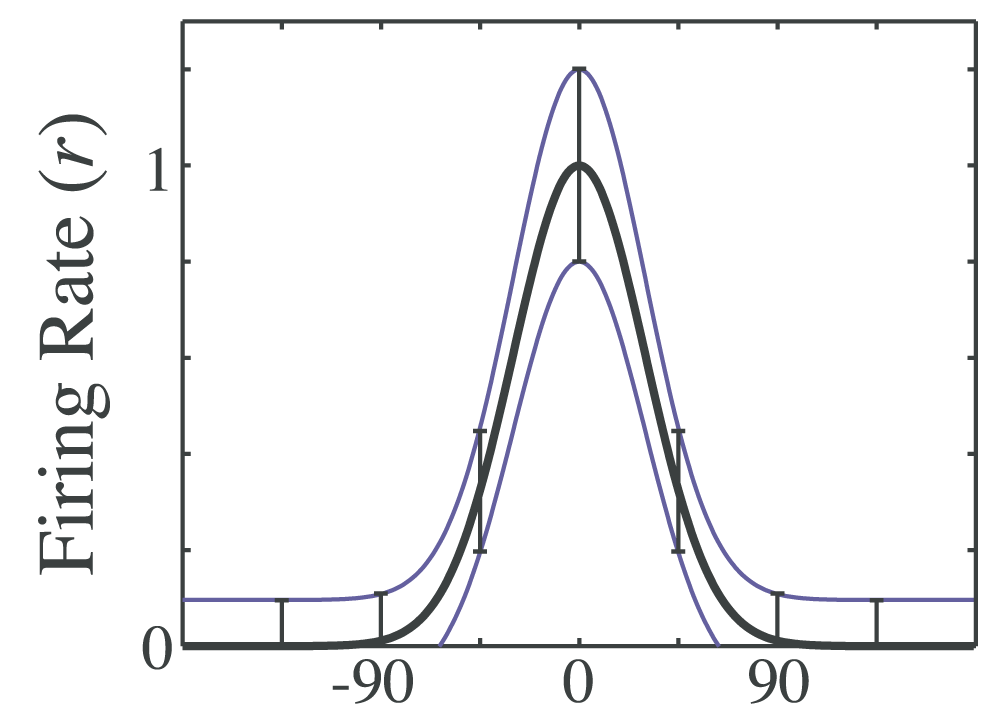
\includegraphics{figures/tuningcurve}
    \end{captionbeside}
\end{figure}

Given a population of neurons, also called a neural \emph{ensemble} in NEF terms, how can the encoded vector $\vc x(t)$ be recovered?
First the activity or spike trains $\act_i(t)$ are convolved with a synaptic filter $\syn$ to obtain the induced post-synaptic voltage change.
Usually this is a decaying exponential $\syn(t) = \syntau^{-1}\exp(-t / \syntau)$, but other filters can be used to more precisely model the dynamics of the synapse \parencite{voelker2017a} and even extensions to conductance-based synapses are possible \parencite{stockel2017}.
From the filtered activity, the represented vector can be reconstructed with a linear, weighted decoding
\begin{equation}
    \hat{\vc x}(t) = \sum_i \dec_i \cdot \sbr{a_i * h}\!(t)
\end{equation}
with decoding weights $\dec_i$.

To get a good reconstruction of the represented value, the decoding weights should minimize the error
\begin{equation}
    E = \int_{\repspace} \norm{\vc x - \hat{\vc x}}^2 \dif \vc x \text{.}
\end{equation}
In general, this minimization cannot be solved analytically.
Thus, in the NEF the integral is approximated by randomly sampling $M$ \emph{evaluation points} $\evalp_k \in \repspace$.
Given the finite number of evaluation points, it becomes possible to solve for the decoding weights with a least-squares minimization.
The detailed derivation is given in \textcite[Ch.~2]{eliasmith2003}.
In short, one obtains the matrices
\begin{equation}
    \actmat = \sbr{\begin{array}{cccc}
            \act_1(\vc x_1) & \act_1(\vc x_2) & \cdots & \act_1(\vc x_M) \\
            \act_2(\vc x_1) & \act_2(\vc x_2) & \cdots & \act_2(\vc x_M) \\
            \vdots & \vdots & \ddots & \vdots \\
            \act_N(\vc x_1) & \act_N(\vc x_2) & \cdots & \act_N(\vc x_M) \\
    \end{array}}
    \ \text{and}\ 
    \evalpmat = \sbr{\begin{array}{c}
            \vc x_1 \\ \vc x_2 \\ \vdots \\ \vc x_M
    \end{array}}
\end{equation}
where one can use the steady-state activities in the activity matrix $\actmat$ which can be obtained analytically for LIF neurons.
Given these two matrices the decoding weights can be obtained with the regularized pseudo-inverse as
\begin{equation}
    \sbr{\begin{array}{c}
            \dec_1\Tr \\ \dec_2\Tr \\ \vdots \\ \dec_N\Tr
        \end{array}} = \del{\actmat \actmat\Tr + M \reg^2 {\max(\actmat)}^2 \imat}^{-1} \actmat \evalpmat
\end{equation}
where $\reg$ is the regularization scale (usually $\reg = 0.1$).

The encoders and decoders not only allow us to encode information into a neural ensembles and decode it back out, but also to transmit that information from one neural population to another.
By decoding from the pre-synaptic ensemble and encoding into the post-synaptic ensemble, the connection weights required between the two populations can be obtained as
\begin{equation}
    \weights_{ij} = \enc_i\Tr \mat T \dec_j
\end{equation}
where $\mat T$ can describe a linear transform to implement across the neural connections.
If $\mat T$ is the identity matrix, the connection will be a pure communication channel.


\section{Transformation}
To be useful, a neural network has to transform or compute functions on the represented information.
In the NEF, it is straight-forward to implement a given transformation in the connection weights between two ensembles.
To implement a function $f(\vc x)$, one replaces the matrix $\evalpmat$ with
\begin{equation}
    \evalpmat_{f(\vc x)} = \sbr{\begin{array}{c}
            f(\vc x_1) \\ f(\vc x_2) \\ \vdots \\ f(\vc x_M)
    \end{array}}
\end{equation}
when solving for decoders.
This corresponds to a minimization of the modified error $E_{f(\vc x)} = \int_{\repspace} \norm{f(\vc x) - \hat{\vc x}}^2 \dif \vc x$.

\Textcite[Ch.~7]{eliasmith2003} shows that a neural network constructed in this way is typically best at computing low-order polynomials.
Non-smooth or discontinuous functions might require a large number of neurons.
In some cases a better function approximation can be achieved by appropriately selecting parameters like intercepts or encoders or by changing the network structure to decompose a function in a different way.
An example is the calculation of products and has been discussed in \textcite{gosmann2015-1}, and \cref{sec:thresholding} shows this for the thresholding of values.

\section{Dynamics}
The final principle of the NEF addresses dynamics.
In linear control theory a dynamical system is often described by state equations of the form
\begin{align}
    \od{\vc x}{t} &= \mat A \vc x(t) + \mat B \vc u(t) \label{eqn:statespace1} \\
    \vc y(t) &= \mat C \vc x(t) + \mat D \vc u(t) \label{eqn:statespace2}
\end{align}
where $\vc x(t)$ is the state vector, $\vc u(t)$ the input vector, and $\vc y(t)$ the output vector.
The system behaviour is determined by the dynamics matrix $\mat A$, input matrix $\mat B$, output matrix $\mat C$, and the feedthrough matrix $\mat D$.
\Cref{fig:statespace} shows a graphical representation.
\begin{figure}
    \centering
    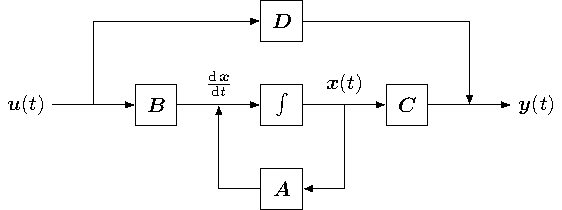
\includegraphics{tikz/statespace}
    \caption{Visualization of \cref{eqn:statespace1,eqn:statespace2} as block diagram.}\label{fig:statespace}
\end{figure}

In the NEF, we want to map a given dynamical system onto neural components (\cref{fig:neural-lti}).
The neuron dynamics are dominated by the synaptic filter \parencite[Appendix~F.1]{eliasmith2003} which becomes the transfer function and gives
\begin{equation}
    \vc x(t) = \syn(t) * \sbr{\mat A' \vc x(t) + \mat B' \vc u(t)} \text{.}
\end{equation}
With help of the Laplace transform one can obtain $\mat A'$ and $\mat B'$ from $\mat A$ and $\mat B$ as
\begin{align}
    \mat A' &= \syntau \mat A + \imat \\
    \mat B' &= \syntau \mat B  \text{.}
\end{align}
This implies that to implement a dynamical system with a neural ensemble, the input has to be multiplied by $\syntau$ to account for the synaptic filtering.
In addition, one needs to add a recurrent transformation implementing the function $f(\vc x) = \syntau \mat A \vc x + \vc x$.
Note that combining this third principle with the principle of transfomation, allows the implementation of nonlinear dynamics in a spiking neural network.
\begin{figure}
    \centering
    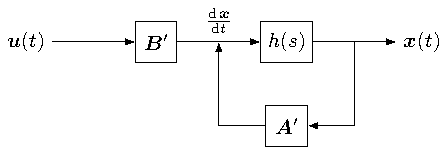
\includegraphics{tikz/neural-lti}
    \caption[Block diagram of the linear system of a neural population.]{Block diagram of the linear system of a neural population. $h(s)$ is the Laplace transformed synaptic filter $\syn(t)$.}\label{fig:neural-lti}
\end{figure}


\section{Simulating NEF networks}
To simulate NEF style networks, I use the Python library Nengo \parencite{bekolay2014,sharma2016}.
It supports different backends to run neural models on different hardware platforms.
For example, Nengo OCL targets GPUs with an OpenCL implementation.
While this allows better simulation performance, special case implementations are necessary for certain features.
In particular, this applies to the association matrix learning rule (see \cref{sec:aml}).
Moreover, I utilized the Sharcnet and Compute Canada high-performance clusters which typically provide more CPU resources than GPU resources.
Thus, I mostly used the Nengo reference (CPU) backend.
To obtain sufficient simulation performance for the size of models constructed in this work, it was necessary to optimize memory organization of the internal data structures of the backend.
While the exact details are out of the scope of this thesis, they are published in \textcite{gosmann2017}.

\chapter{Basic NEF networks}
When constructing neural models with the NEF, there are certain networks that are often used in multiple places and constitute some basic building blocks in a sense.
In the following we will shortly discuss how to create an integrator, a gated memory buffer based on that integrator, an ensemble applying a threshold to a signal, and how to do multiplication in neurons.

\section{Integrator}
Integrators are important components in many NEF models because they allow to store values over some timespan in neural activity.
An integrator is described by the differential equation
\begin{equation}
    \od{\vc x(t)}{t} = \vc u(t)
\end{equation}
where $\vc u(t)$ is the external input to the integrator.
Applying principle 3 of the NEF tells us that the input has to be scaled by the synaptic time constant $\tausyn$.
Furthermore, a recurrent connection feeding the output of the integrator back to itself is needed.
To get a stable representations over a sufficient time window, it is best to use a long time constant like $\tausyn = \SI{0.1}{\second}$ which is the range measured for the TODO neurotransmitter.
Due to neural noise and distortion error, the represented value can drift over time.
Adding more neurons to the integrator will make it more stable.
TODO figures

\section{Gated memory buffer}
While the integrator enables us to store a value over time, it does not allow for particularly quick updating.
A quicker update can be achieved by adding a difference ensemble (TODO figure).
By scaling the difference with a factor the updating speed can be regulated.
However, too large values will lead to oscillations in the integrator.
Note that in this case feeding a null vector to the difference ensemble will clear out the memory instead of keeping the current value.
Thus, the input the integrator needs to be gated.
This can be done by inhibiting the neurons of the difference ensemble to keep the current value in the integrator.

\section{Thresholding ensembles}
Often one needs to apply a threshold to value, i.e.\ implement the function
\begin{equation}
    f(x) = \left\{ \begin{array}{ll}
            0 & x < 0 \\
            x & x \geq 0
        \end{array} \right.
    \text{,}
\end{equation}
or compute the Heaviside step function
\begin{equation}
    \Heavi(x) = \left\{ \begin{array}{ll}
            0 & x < 0 \\
            1 & x \geq 0
        \end{array} \right.
    \text{.}
\end{equation}
Both of these functions are non-differentiable at 0.
The Heaviside function is even discontinuous at that spot.
These properties make it problematic to implement this function with a standard NEF ensemble.
Nevertheless, a good approximations of these functions can be achieved by aligning the neuron's tuning curves according to the shape of these functions.

Instead of choosing encoders randomly as $-1$ and $1$, all encoders are set to $1$ and all intercepts are chosen from $x \in [0; 1]$.
Choosing the intercept distribution of this interval appropriately can further increase the accuracy.
An exponential distribution that clusters intercepts close to 0 performs best.
Note that this is even better than setting all intercepts to 0 as this gives more variation in the tuning curves.
The uniform distribution often does not produce intercepts close enough to the threshold value which leads to an increased effective threshold.

TODO figures

\section{Product}
A product of two scalar numbers $x$ and $y$ could be computed by feeding them into separate dimensions of a two-dimensional ensemble and decoding out the product.
A \SI{37}{\percent} more accurate implementation (with the same number of neurons) is, however, possible (TODO ref) by rewriting the product with squares as
\begin{equation}
    xy = \frac{1}{4}\del{x^2 + 2xy + y^2} - \frac{1}{4}\del{x^2 - 2xy + y^2} = \frac{1}{4}\del{x + y}^2 - \frac{1}{4}\del{x - y}^2 \text{.}
\end{equation}
The neural implementation of this equation is straight-forward (TODO figure).

Multiple scalar product networks can be combined to compute element-wise vector products.
By summing across those element-wise products a dot product can be computed.
Product networks are also used in the computation of circular convolution as binding operation in the Semantic Pointer Architecture (TODO ref section).

\chapter{The Semantic Pointer Architecture}\label{sec:spa}
While the Neural Engineering Framework allows us to encode vectors into spiking neural networks and transform them, it does not tell us how to use those vectors to represent structured, conceptual, or symbol-like information.
Different such methods could be devised, though in the context of the NEF the most widely used method is the Semantic Pointer Architecture \parencite[SPA;][]{eliasmith2013}.
The SPA has been used to build a multitude of cognitive models, including the n-back task \parencite{gosmann2015}, the Tower of Hanoi task \parencite{stewart2011-2}, human-scale knowledge representation \parencite{crawford2016}.
The largest and most complex example of a SPA model is Spaun, the Semantic Pointer Architecture Unified Network, combining eight different tasks in a single functional spiking-neuron model \parencite{Eliasmith2012}.

The conceptual representations in the SPA are a specific instance of a Vector Symbolic Architecture \parencite[VSA;][]{gayler2004}.
In VSAs concepts are represented with vectors, and linear and nonlinear operators are used to combine basic concepts in more complex structured representations.
Three types of operators are considered essential in a VSA\@.
First, a measure of similarity
\begin{equation}
    \simmeasure: \mathbb{R}^{\dims} \times \mathbb{R}^{\dims} \longrightarrow \mathbb{R}
\end{equation}
for which I use the normalized dot product (also known as cosine similarity)
\begin{equation}
    \simmeasure(\vc x, \vc y) := \frac{\left\langle \vc x, \vc y \right\rangle}{\norm{\vc x} \cdot \norm{\vc y}}
\end{equation}
for the remainder of this thesis.
Second, a superposition operator
\begin{equation}
    \superpos: \mathbb{R}^{\dims} \times \mathbb{R}^{\dims} \longrightarrow \mathbb{R}^{\dims}
\end{equation}
is required that produces a vector similar to both inputs, i.e., $\simmeasure(\superpos(\vc x, \vc y), \vc x) \approx \simmeasure(\superpos(\vc x, \vc y), \vc y) \gtrapprox \sqrt{1/2}$ for $\simmeasure(\vc x, \vc y) \approx 0$.
This is usually, and will be for the remainder of this thesis, simple elementwise addition, i.e., $\superpos(\vc x, \vc y) := \vc x + \vc y$.
Finally, a binding operator
\begin{equation}
    \bind: \mathbb{R}^{\dims_1} \times \mathbb{R}^{\dims_2} \longrightarrow \mathbb{R}^{\dims}
\end{equation}
is needed with an approximate inverse or unbinding operation
\begin{equation}
    \bind^+: \mathbb{R}^d \times \mathbb{R}^{\dims_2} \longrightarrow \mathbb{R}^{\dims_1} \text{.}
\end{equation}
To be able to build up and retrieve information from representations, the binding and unbinding operations are required to be distributive, i.e.,
\begin{align}
    \bind(\vc x + \vc y, \vc z) &= \bind(\vc x, \vc z) + \bind(\vc y, \vc z) \\
    \bind^+(\vc x + \vc y, \vc z) &= \bind^+(\vc x, \vc z) + \bind^+(\vc y, \vc z) \text{.}
\end{align}

For some proposed binding operations, like Tensor products \parencite{smolensky1990}, the unbinding operation is the exact inverse $\bind^+ = \bind^{-1}$ with
\begin{equation*}
    \bind^{-1}(\bind(\vc x, \vc y), \vc y) = \vc x \text{.}
\end{equation*}
However, Tensor products increase the vector dimensionality with each successive binding which leads to biological implausible scaling problems \parencite[Appendix D.5]{eliasmith2013}.
For that reason, I only consider binding methods that keep the dimensionality $\dims = \dims_1 = \dims_2$ constant.

In pure math, it is still possible to define binding operators with an exact inverse, but we need to keep the implementation in neurons in mind.
This introduces additional constraints.
First, the actual usable representational space $\repspace \subsetneq \mathbb{R}^{\dims}$ is limited, constraining unlimited growth of bound vectors.
Second, neural noise limits the representational accuracy, preventing highly non-linear operators.
It follows that for a binding operator in a neural system it is desired to maximize the set $\mathcal{V} \subseteq \repspace$ for which  $\simmeasure(\bind^+(\bind(\vc x, \vc y) + \vc\zeta, \vc y), \vc x) \approx 1$ for all $\vc x, \vc y \in \mathcal{V}$ and samples of noise $\vc\zeta$ in the neural system.
Note that this condition would be satisfied by using the identity $\bind(\vc x, \vc y) = \bind^+(\vc x, \vc y) = \vc x$.
Thus, simultaneously it needs to hold that $\simmeasure(\bind^+(\bind(\vc x, \vc y), \vc z), \vc x) \approx 0$ for all $\vc x, \vc y, \vc z \in \mathcal{V}$ with $\simmeasure(\vc y, \vc z) \approx 0$.
At this point, it is useful to introduce three more definitions.

\begin{defn}[identity vector]
    A vector $\bid_{\bind}$ with the property $\bind(\vc x, \bid_{\bind}) = \vc x$ is called \emph{identity vector} under $\bind$.
\end{defn}
\begin{defn}[absorbing element]
    A vector $\bzero_{\bind}$ with the property $\bind(\vc x, \bzero_{\bind}) = c \cdot \bzero_{\bind}$ where $c \in \mathbb{R}$ is called an \emph{absorbing element} under $\bind$.
\end{defn}
Such an absorbing element effectively destroys the information in the vector $\vc x$.
For that reason, absorbing elements should be avoided when constructing representations with binding.
Note that this definition slightly differs from the usual definition of absorbing elements by allowing for a scaling factor.
\begin{defn}[unitary vector]
    A vector $\vc u$ with the property $\langle \bind(\vc x, \vc u), \bind(\vc y, \vc u) \rangle = \langle \vc x, \vc y \rangle$ is called unitary.
\end{defn}
In other words, a unitary vector preserves the dot product under binding.
This is in analogy to unitary transformation matrices that also preserve the dot product.
It also implies that binding with a unitary vector preserves the length of the bound vector.


\section{Binding operations}
I introduce two specific binding operations now.
First, circular convolution is discussed, which has been the binding operation of choice in the SPA so far.
Second, I introduce a new binding method, termed vector-derived transformation binding, with some trade-offs.
The two binding approaches and their suitability for different problems is discussed.

\subsection{Circular convolution}
The binding operator classically used in the SPA is circular convolution, and was suggested by \textcite{plate1995,plate2003} for his Holographic Reduced Representations (HRRs).
\begin{defn}[circular convolution binding]
    The circular convolution binding operator is given by
    \begin{equation}
        \bind_{\circledast}(\vc x, \vc y) := \vc x \circledast \vc y\ \text{with}\ \del{\vc x \circledast \vc y}_i = \sum_{j=0}^{d - 1} x_j y_{(i - j) \bmod d}
    \end{equation}
    and has the approximate inverse \parencite{plate2003}
    \begin{equation}
        \bind^+_{\circledast}(\vc x, \vc y) = \vc x \circledast \vc y^+\ \text{with}\ \vc y^+ := \del{y_0, y_{d-1}, y_{d-2}, \dotsc, y_1}\Tr \text{.}
    \end{equation}
\end{defn}

The basic properties of
\begin{align}
    &\text{distributivity:} &(\vc x_1 + \vc x_2) \circledast \vc y &= \vc x_1 \circledast \vc y + \vc x_2 \circledast \vc y \text{,}\\
    &\text{associativity:} &(\vc x \circledast \vc y) \circledast \vc z &= \vc x \circledast (\vc y \circledast \vc z) \text{,} \\
    &\text{commutativity:} &\vc x \circledast \vc y &= \vc y \circledast \vc x
\end{align}
hold for circular convolution as a binding operator.
A useful property of circular convolution for the implementation in a neural network with the NEF is, that it becomes element-wise multiplication in the Fourier space defined by
\begin{equation}
    \vc x \circledast \vc y = \fouriermat^{-1}\sbr{(\fouriermat \vc x) \circ (\fouriermat \vc y)}
\end{equation}
where $\fouriermat$ is the discrete Fourier transform (DFT) matrix.
The linear transform with the DFT matrix can be put easily into the neural connection weights and the element-wise product can be done with a well-optimized product network \parencite{gosmann2015-1}.

The expression in Fourier space also allows the derivation of the special elements of circular convolution.
The identity vector must not change the complex Fourier coefficient in the element-wise multiplication.
Thus, its Fourier coefficients must all be $1 + 0\iu$ and the identity vector is given by
\begin{equation}
    \bid_{\circledast} = (1, 0, 0, \dotsc, 0)\Tr \text{.}
\end{equation}
Furthermore, all vectors with Fourier coefficients $c_n \in \mathbb{C}$ that have an absolute value of $\left|c_n\right| = 1$ are unitary, as one can easily verify.
A trivial example of a unitary vector is the identity vector $\bid_{\circledast}$.
Finally, all vectors $(z, \dotsc, z)\!\Tr$ with $z \in \mathbb{R}$ are absorbing elements.

\subsection{Vector-derived transformation binding}
Circular convolution can be interpreted as moving one of the operands around in the $d$-dimensional space in a way defined by the other operand.
This leads to the question, whether there are other ways to project one vector to a new location based on the other vector.
One such way is what I call \emph{vector-derived transformation binding (VTB)}, which to my knowledge has not been described before.
\begin{defn}[vector-derived transformation binding, VTB]
    Given a $\dims' = \dims^{\frac{1}{2}} \in \posnum$, the vector-derived transformation binding operator $\vtb: \mathbb{R}^{\dims} \times \mathbb{R}^{\dims} \longrightarrow \mathbb{R}^{\dims}$ is defined as
    \begin{equation}
        \vtb(\vc x, \vc y) := \bar{\mat V}_{\vc y} \vc x = \begin{bmatrix}
            \mat V_{\vc y} & 0 & 0 \\
            0 & \mat V_{\vc y} & 0 \\
            0 & 0 & \ddots
        \end{bmatrix} \vc x
    \end{equation}
    with
    \begin{equation}
        \mat V_{\vc y} = \dims^{\frac{1}{4}} \begin{bmatrix}
            y_1 & y_2 & \dotso & y_{\dims'} \\
            y_{\dims' + 1} & y_{\dims' + 2} & \dotso & y_{2\dims'} \\
            \vdots & \vdots & \ddots & \vdots \\
            y_{\dims - \dims' + 1} & y_{d - \dims' + 2} & \dotso & y_{\dims}
        \end{bmatrix} \text{.}
    \end{equation}
    The approximate inverse is given by
    \begin{equation}
        \vtb^+(\vc x, \vc y) = \bar{\mat V}_{\vc y}\Tr \vc x = \begin{bmatrix}
            V_{\vc y}\Tr & 0 & 0 \\
            0 & V_{\vc y}\Tr & 0 \\
            0 & 0 & \ddots
        \end{bmatrix} \vc x \text{.}
    \end{equation}
\end{defn}
This binding method is based on the fact that in the SPA vectors are usually randomly generated and uniformly distributed with identically distributed components.
In that case each subvector (e.g., each row in $\mat V_{\vc y}$) is also uniformly distributed with identically distributed components.
Furthermore, for high-dimensional vector spaces almost all (uniformly sampled) vectors are orthogonal and semantic pointers are usually picked to have unit-length.
Thus, the matrix $\bar{\mat V}_{\vc y}$ is almost orthogonal with the implication $\bar{\mat V}_{\vc y}\Tr \bar{\mat V}_{\vc y} \approx \imat$.
Vectors $\vc y$ that give a perfectly orthogonal matrix $\mat V_{\vc y}$, are unitary.
One special unitary vector is the identity vector.
\begin{corollary}[VTB identity vector]
    The identity vector for VTB is given by
    \begin{equation}
        \sbr{\bid_{\ped{V}}}_i = \left\{ \begin{array}{ll}
                \dims^{-\frac{1}{4}} & i \in \cbr{(k - 1) \dims' + k : k \leq \dims', k \in \mathbb{N}_{>0}} \\
                0 & \text{otherwise}
        \end{array}\right. \text{.}
    \end{equation}
    \begin{proof}
        By writing $\bid_{\ped{V}}$ as $\mat V_{\bid_{\ped{V}}}$ one can easily verify that $\mat V_{\bid_{\ped{V}}} = \imat\ \Rightarrow\ \bar{\mat V}_{\bid_{\ped{V}}} = \imat$.
    \end{proof}
\end{corollary}
Example for $d = 9$: $\bid_{\ped{V}}^{(9)} = (1, 0, 0, 0, 1, 0, 0, 0, 1)\Tr$.

\begin{corollary}[VTB distributivity]
    VTB is distributive:
    \begin{equation}
        \begin{split}
            \vtb(\vc x_1 + \vc x_2, \vc y) &= \vtb(\vc x_1, \vc y) + \vtb(\vc x_2, \vc y) \text{ and}\\
            \vtb(\vc x, \vc y_1 + \vc y_2) &= \vtb(\vc x, \vc y_1) + \vtb(\vc x, \vc y_2) \text{.}
        \end{split}
    \end{equation}
    \begin{proof}
        By applying the definitions for both directions of the distributivity:
        \begin{itemize}
            \item $\vtb(\vc x_1 + \vc x_2, \vc y) = \bar{\mat V}_{\vc y} \del{\vc x_1 + \vc x_2} = \bar{\mat V}_{\vc y} \vc x_1 + \bar{\mat V}_{\vc y} \vc x_2 = \vtb(\vc x_1, \vc y) + \vtb(\vc x_2, \vc y)$
            \item $\vtb(\vc x, \vc y_1 + \vc y_1) = \bar{\mat V}_{\vc y_1 + \vc y_2} \vc x = \del{\bar{\mat V}_{\vc y_1} + \bar{\mat V}_{\vc y_2}} \vc x = \bar{\mat V}_{\vc y_1} \vc x + \bar{\mat V}_{\vc y_2} \vc x = \vtb(\vc x, \vc y_1) + \vtb(\vc x, \vc y_2)$
    \end{itemize}
    \end{proof}
\end{corollary}
In contrast to circular convolution, VTB is neither commutative
\begin{equation}
    \vtb(\vc x, \vc y) = \bar{\mat V}_{\vc y} \vc x \neq \bar{\mat V}_{\vc x} \vc y = \vtb(\vc y, \vc x) \text{,}
\end{equation}
nor associative
\begin{equation}
    \vtb(\vc x, \vtb(\vc y, \vc z)) = \bar{\mat V}_{\bar{\mat V}_{\vc z} \vc y} \vc x \neq \bar{\mat V}_{\vc z} \bar{\mat V}_{\vc y} \vc x = \vtb(\vtb(\vc x, \vc y), \vc z) \text{.}
\end{equation}
This implies that unlike circular convolution, multiple bindings cannot be undone in a single step, but a separate unbinding step is required for each binding.
Despite the non-commutativity, it is possible to flip the operands in the bound state $\vtb(\vc x, \vc y) = \mat V_{\leftrightarrow} \vtb(\vc y, \vc x)$ with the matrix
\begin{equation}
    \sbr{\mat V_{\leftrightarrow}}_{ij} = \left\{ \begin{array}{ll}
            1 & j = 1 + \left\lfloor \frac{i - 1}{\dims'} \right\rfloor + \dims' \sbr{\del{i - 1} \bmod \dims'} \\
            0 & \text{otherwise}
        \end{array}\right. \text{.}
\end{equation}
Example for $d = 4$:
\begin{equation*}
    \mat V_{\leftrightarrow}^{(4)} = \sbr{\begin{array}{cccc}
            1 & 0 & 0 & 0 \\
            0 & 0 & 1 & 0 \\
            0 & 1 & 0 & 0 \\
            0 & 0 & 0 & 1
        \end{array}}
\end{equation*}

\subsection{Comparison of circular convolution and vector-derived transformation binding}
Both circular convolution and VTB are compressed binding operations.
Because of the lossy compression, we lose some information in each binding which makes it increasingly harder to recover the original unbound vectors.
To combat this effect (and the effect of neuron noise) clean-up memories like the one by \textcite{stewart2011} are required.
Likewise the independent accumulator model discussed in \cref{sec:ia} can be used as a clean-up memory.

In addition to the information loss, the binding operations change the length of the vector (if neither operand is unitary).
This can be a problem in a neural representation as neurons saturate and might not represent the vector accurately anymore.
In particular, neural ensembles in the NEF are optimized for a certain representational space, usually a hyperball with a given radius $\radius$.
It is convenient to set $\radius = 1$ and try to keep the Semantic Pointer vectors at unit-length.

\Cref{fig:bindings-autoconv} shows how the mean length of random vectors repeatedly bound with themselves changes.
For the circular convolution the length increases much faster than for VTB\@.
Such a rapid increase in length can be problematic in a neural network with a limited representational radius as in the NEF\@.
Moreover, VTB preserves more information of the bound vectors as shown by the similarity to the original vectors when undoing all bindings.
After repeated binding with itself and then the same number of unbindings, the resulting VTB bound vector is more similar to the original vector than the circular convolution bound vector.
\begin{figure}
    \centering
    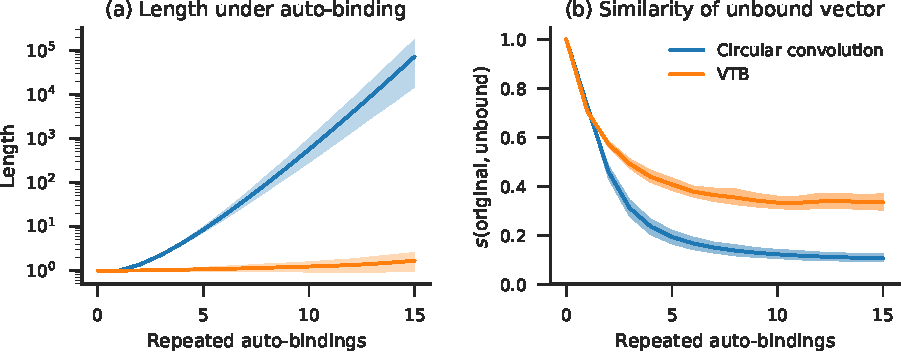
\includegraphics{figures/bindings-autoconv}
    \caption[Repeatedly binding a 256-dimensional vector with itself.]{Repeatedly binding a 256-dimensional vector with itself. (a) Length of the resulting vector. (b) Similarity of the original vector to the vector obtained when undoing all bindings. The shaded areas represent \SI{95}{\percent} confidence intervals.}\label{fig:bindings-autoconv}
\end{figure}

While binding vectors with themselves can sometimes be useful (e.g., for generating Semantic Pointers with a successive relationship like position indices), it is much more common to bind randomly sampled vectors.
\Cref{fig:bindings-random} shows the same experiment where a random vector was used in each binding.
In this case, the vector length decreases to zero, even if it might increase in some of the early bindings.
Again, this decrease is much quicker for circular convolution binding than for VTB and the latter method also preserves more of the similarity across bindings.
\begin{figure}
    \centering
    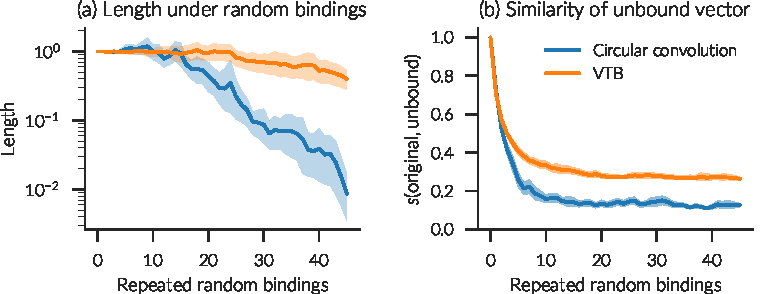
\includegraphics{figures/bindings-random}
    \caption[Repeatedly binding a 256-dimensional vector with random vectors.]{Repeatedly binding a 256-dimensional vector with random vectors. (a) Length of the resulting vector. (b) Similarity of the original vector to the vector obtained when undoing all bindings. The shaded areas represent \SI{95}{\percent} confidence intervals.}\label{fig:bindings-random}
\end{figure}

It is conceivable that the problems with scaling of the vector length can be fixed by normalizing after each binding.
This, however, does not affect the loss of information in each binding (\cref{fig:bindings-normalized}).
Also, implementing normalization in a neural network is notoriously difficult because of the division involved with an unbounded output as the divisor approaches zero.
Good approximations of normalization are only possible for a defined and finite input range.
It is worth noting that the neurons in the NEF perform a sort of ``soft normalization'' for large values, as the neuron's firing rates saturate.
But this only affects vectors exceeding a certain length and can lead to other distortions in the representation.
\begin{figure}
    \centering
    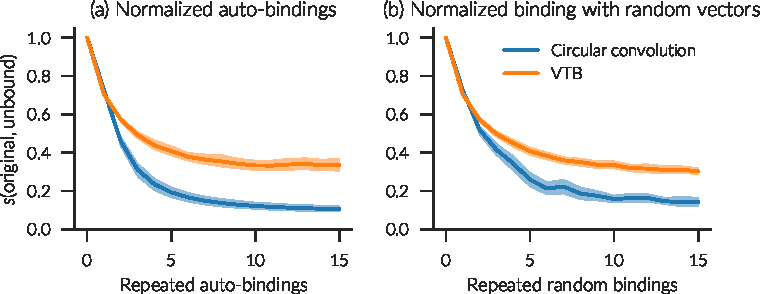
\includegraphics{figures/bindings-normalized}
    \caption[Repeatedly binding a 256-dimensional vector with normalization.]{Repeatedly binding a 256-dimensional vector with (a) itself or (b) random vectors and normalizing in each step. The similarity to the original vector after undoing all bindings is shown. The shaded areas represent \SI{95}{\percent} confidence intervals.}\label{fig:bindings-normalized}
\end{figure}

Another approach to preventing the growth or decay of the vector length, and even prevent the information loss, is the usage of unitary vectors.
These keep the vector length constant and perform lossless binding due to their perfect inverse.
Note that binding two unitary vectors gives another unitary vector.
Thus, repeated binding is not a problem.
However, the scaling properties of VSAs are based on the fact that the number of almost orthogonal vectors that fits into a vector space grows exponentially with the dimensionality of that space \parencite{wyner1967,cai2013}.
Because not all vectors are unitary, this scaling property might be lost when restricted to unitary vectors.
It might be best to use unitary vectors only for those Semantic Pointers that are repeatedly used in bindings.
But it is also worth keeping in mind that achieving the theoretical limit of almost orthogonal vectors in a space is a hard problem, closely related to sphere packing and unsolved for arbitrary dimensionality \parencite{cohn2017}.
Thus, the practical scaling of the number of useable vectors might be less then the exponential scaling for both unitary and non-unitary vectors.

So far VTB looks like the better choice for a binding operation.
But it does not come not without downsides.
In contrast to circular convolution, it is not associative or commutative.
While the desirability of commutativity depends on the employed representation scheme, the non-associativity implies that each binding has to be undone in an individual step, while circular convolution allows us to undo a chain of bindings in a single step, if the vector representing that chain is available.
Thus, circular convolution can allows the recovery of information more quickly.
Ultimately, this is a question of what binding operations the brain applies for different forms of processing (if such binding is at all related to what the brain does).
Potentially, the binding operations lead to different timing predictions, as unbinding with the VTB may take more time.
Deriving such predictions and testing them experimentally is, however, out of the scope of this thesis.

Finally, we have to consider the neural implementation of these binding operations.
Both essentially require a set of multiplication networks.
For the circular convolution, the DFT (and inverse DFT) can be implemented in feed-forward connection weights that do not require any additional neurons.
For each of the input vectors $\dims$ Fourier complex coefficients are produced, but as the inputs are real-valued, half of these are the complex conjugate of the other half.
Thus, only $\dims / 2$ coefficients have to be considered.
Each coefficient is a complex number multiplied with one coefficient of the other vector.
That results in four real-valued multiplies per coefficient.
In total, $2\dims$ multiplications are required for a circular convolution.
For VTB, there are $\dims^{1/2}$ multiplications of $\dims^{1/2} \times \dims^{1/2}$ matrices with a vector, resulting in a total of $\dims^{3/2}$ multiplications.
However, each column vector in $\bar{\mat V}_{\vc y}$ gets scaled by the same component of $\vc x$.
That would allow, to store each of these column vectors in a single NEF ensemble with the respective $x_i$ in an additional dimension, and then decode the scaled column vector.
This requires only $\dims$ ensembles to decode from, but each ensemble needs to represent $\dims^{1/2} + 1$ dimensions, and to keep the noise error constant (as discussed in the next chapter), the number of neurons in each ensemble then needs to be scaled by ${(\dims^{1/2} + 1)}^{3/2} \approx \dims^{3/4}$.
Overall ensembles this amounts to a scaling by $\dims^{7/4}$.
Thus, the VTB requires more neural resources.
It should be noted, that for either binding method, the binding with a fixed vector can be implemented purely in the connection weights as it reduces to a simple matrix multiplication in either case.

Despite VTB having many advantages over circular convolution, I decided to use circular convolution in the memory model.
The main reason is that support for circular convolution is already implemented in Nengo and the model does not use a lot of binding operations.
Nevertheless, it would be interesting to switch the model over to VTB and investigate effects on the performance in the future.


\section{Structured representations}
Once we defined a binding operation, it can be used to build up structured representations with Semantic Pointers.
For example, consider a scene with a red square and blue circle that we want to encode as Semantic Pointer.
Assume that we have Semantic Pointers \spc{red}, \spc{square}, \spc{blue}, and \spc{circle}.
One possible encoding would be
\begin{equation}
    \vc s = \bind(\spc{red}, \spc{square}) + \bind(\spc{blue}, \spc{circle}) \text{.}
\end{equation}
We could then recover the color of the square as
\begin{align}
    \bind^+(\vc s, \spc{color}) &= \bind^+(\bind(\spc{red}, \spc{square}), \spc{square}) + \bind^+(\bind(\spc{blue}, \spc{circle}), \spc{square}) \\
    &\approx \spc{red} + \mathrm{noise} \text{.}
\end{align}
Note, however, that the binding operation needs to be commutative to recover the shape from the color with this encoding scheme.
Other encoding schemes can be devised to alleviate this concern.
For example, the properties can be bound to a role and each object to an object identifier:
\begin{align}
    \vc o_1 &= \bind(\spc{red}, \spc{color}) + \bind(\spc{square}, \spc{shape}) \\
    \vc o_2 &= \bind(\spc{blue}, \spc{color}) + \bind(\spc{circle}, \spc{shape}) \\
    \vc s &= \bind(\vc o_1, \spc{obj}_1) + \bind(\vc o_2, \spc{obj}_2) \text{.}
\end{align}
To find the color of a specific shape, each object would have to be retrieved, then the shape of the object to compare it to the target shape, and finally the color has to recovered if the shape matches.
Thus, different encoding schemes can lead to different timing predictions.
The latter approach requires scanning and through multiple objects and thus it should take longer to recover information with more items, while the former approach can recover any property in a single step.
Despite those differences, both encoding approaches are similar, in so far as pairs of semantic pointers are bound together.
\begin{defn}[encoding with binding]
    Given $k$ pairs $(\vc x_i, \vc y_i) \in \mathbb{R}^{\dims} \times \mathbb{R}^{\dims}$, the encoding of these pairs into a single Semantic Pointer $\vc m$ with binding is given by
    \begin{equation}
        \vc m = \sum_{i=1}^k \bind(\vc x_i, \vc y_i) \text{.}
    \end{equation}
\end{defn}
An $\vc x_i$ from such a trace can be recalled as $\vc x_i \approx \hat{\vc x}_i = \bind^+(\vc m, \vc x_i)$.
While most concrete encoding schemes make use of encoding with binding, at least one other method, encoding with tagging, has been proposed \parencite{recchia2015}.
\begin{defn}[encoding with tagging]
    Given $k$ pairs $(\vc x_i, \vc y_i) \in \mathbb{R}^{\dims} \times \mathbb{R}^{\dims}$ and a matrix $\mat M \in \mathbb{R}^{\dims \times \dims}$ with an approximate inverse $\mat M^+$ satisfying $\mat M^+ \mat M \approx \imat$, the encoding into a single Semantic Pointer with tagging is given by
    \begin{equation}
        \vc m = \sum_{i=1}^k \mat M^{2i-1} \del{\vc y_i + \mat M \vc x_i} = \sum_{i=1}^k \mat M^{2i-1} \vc y_i + \mat M^{2i} \vc x_i \text{.}
    \end{equation}
\end{defn}
The retrieval of an $\vc x_i \approx \hat{\vc x}_i$ is accomplished with
\begin{align}
    \hat{\vc x}_i &:= \del{\mat M^{2c}}^+ \vc m \\
    c &= \argmax_{j \in \sbr{1, k}}\ \simmeasure\!\del{\vc y_i, \del{\mat M^{2j-1}}^{\!+} \vc m} \text{.}
\end{align}

There are a number of sensible choices for the matrix $\mat M$.
\begin{itemize}
    \item First of all, for both, circular convolution and VTB, binding with a \emph{fixed} vector $\vc v$ can be expressed as a matrix multiplication.
        A matrix $\mat M$ derived in this way is unitary, if and only if the vector $\vc v$ is unitary for the given binding operation.
    \item A common choice for encoding with tagging are permutation matrices.
        These are unitary and an exact inverse is given by the transpose.
    \item A special permutation matrix is the matrix that shifts all vector components by one.
        For a given permutation matrix, the vector space dimensions can be reordered such that the permutation matrix becomes the shift by one.
        Interestingly, the shift by one is also equivalent to a circular convolution with the vector $(0, 1, 0, 0, \dotsc)\Tr$.
    \item Other good candidates for $M$, that have not been considered to my knowledge, are (random) orthogonal matrices.
        These are unitary operators on $\mathbb{R}^{\dims}$ and thus have an exact inverse given by the transpose.
\end{itemize}
The relations of these different matrix choices is shown in the Venn diagram in \cref{fig:tagging-matrices}.
\begin{figure}
    \centering
    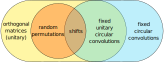
\includegraphics[scale=0.85]{figures/tagging-matrices}
    \caption[Venn diagram of matrices for encoding with tagging.]{Venn diagram of the relations between different classes of matrices $\mat M$ that can be used for encoding with tagging.}\label{fig:tagging-matrices}
\end{figure}

Either encoding method allows the recovery of encoded vectors, but the encoding vector itself is (in general) not similar to those encoded vectors.
In this way, the vector is analogous to a pointer in computer science that doesn't directly contain the information, but can be dereferenced to access the information it is pointing to.
Unlike pointers, however, these vectors can also capture semantic information by their distance in vector space.
Due to the combination of these two facts, these vectors are called Semantic Pointers. 


\subsection{Comparison of encoding methods}
Based on experiment~1 from \textcite{recchia2015}, the encoding methods can be compared by measuring the pairwise binding capacity.
To do so, a set of \num{1000}~vectors with normally distributed components $x_i \sim \ndist\!\del{\!0, \sqrt{1/\dims}}$ are created (note that $\expected\!\sbr{\,\norm{\vc x}} = 1$).
From this set \num{500}~pairs are sampled with replacement.
Then $k$ of these pairs are encoded into a single vector and it is tested whether the $\vc x$ of a random encoded pair $(\vc x, \vc y)$ can recovered with the cue $\vc y$.
A vector counts a successfully recovered if $\hat{\vc x}$ is more similar to $\vc x$ than any other vector in the initial set of vectors.
\num{1000} trials were run and averaged over for each encoding scheme and vector dimensionality.
Because VTB requires the dimensionality~$\dims$ to be square, \num{256}, \num{484}, \num{1024}, and \num{2025} were picked.

\Cref{fig:encoding}a shows the results for encoding with binding.
Both binding operators perform about the same.
While this experiment essentially follows \textcite{recchia2015}, it gives much better results.
It is not clear whether they omitted an essential detail from their description or whether their implementation of the binding operation is flawed.
\begin{figure}
    \centering
    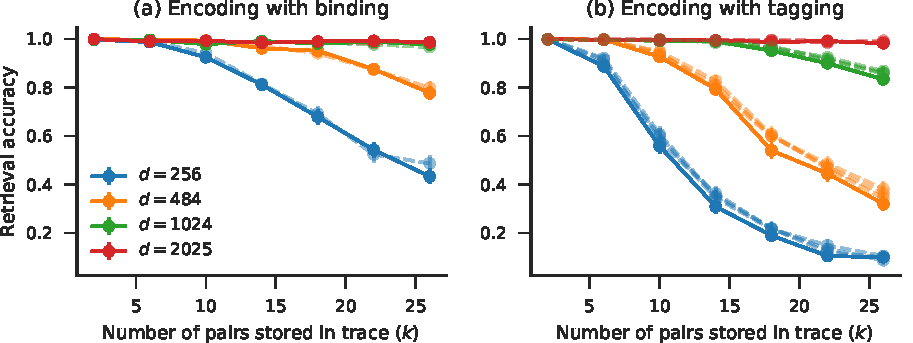
\includegraphics{figures/encoding}
    \caption[Retrieval accuracy of encoding methods.]{Retrieval accuracy for (a) encoding with binding and (b) encoding with unitary tagging matrices. Solid lines show results for VTB\@. The dashed lines in (a) show results for binding with circular convolution, in (b) results for unitary circular convolution matrices, shift matrices, and orthogonal matrices without further indication as the results are almost identical. Error bars denote \SI{95}{\percent} confidence intervals.}\label{fig:encoding}
\end{figure}

The results for encoding with tagging by a shift of one are shown in \cref{fig:encoding}b and closely match the results presented in \textcite{recchia2015}.
Note that the same result applies to any other permutation matrix as the vector components can be reordered accordingly.
Very similar results are obtained with orthogonal matrices, fixed unitary circular convolution, and unitary VTB\@.
In all these cases, the pairwise binding capacity is below the encoding with binding, opposed to what \textcite{recchia2015} reported.
Intuitively, this can be explained by the fact that encoding with binding is a sum of $k$ vectors, where each vector has encoded information about the pair's constituents, whereas encoding with tagging is a sum of $2k$ vectors because each pair's constituent gets encoded separately.
In other words, encoding with binding has a pairwise binding capacity about twice as high as encoding with tagging.
In the plots, the retrieval accuracies for encoding with binding at $2k$ matches roughly with the retrieval accuracy with tagging at $k$, illustrating this fact.

Finally, we can observe (\cref{fig:encoding-nonunitary-tagging}) that encoding with tagging completely fails with fixed non-unitary circular convolution matrices and does not do much better with non-unitary VTB matrices either.
This is likely due to the fact that repeated circular convolution with the same (non-unitary) vector leads to a super-exponential increase in length.
That causes one pair (or even one vector of that pair) to be much stronger than all the other pairs, preventing their recovery.
\begin{figure}
    \centering
    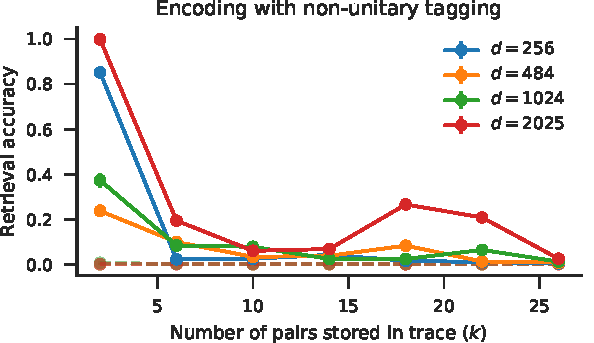
\includegraphics{figures/encoding-nonunitary-tagging}
    \caption[Retrieval accuracy of encoding with non-unitary tagging matrices.]{Retrieval accuracy for encoding with non-unitary tagging matrices. Solid lines show results for VTB matrics, while dashed lines show results for circular convolution matrices. Error bars for \SI{95}{\percent} confidence intervals are smaller than then marker size.}\label{fig:encoding-nonunitary-tagging}
\end{figure}

These experiments clearly show that encoding with binding is preferable.
Even more so, as retrieving items from an encoding with tagging is much more involved.
Each potential cue vector $\vc y_i$ has to be recovered and compared to the actual cue $\vc y$ to determine the maximum similarity to the cue, and which $\vc x_i$ has to be decoded from the encoding.
The encoding with binding allows direct querying of an $\vc x_i$ with a given $\vc y_i$.
This makes for a simpler implementation in a neural network.
That being said, if the main concern is not the implementation in a neural network, but the performance of the vector operations on a classical digital computer, one might come to a different conclusion as \textcite{recchia2015} did.

\chapter{Optimized high-dimensional representation in spiking neurons}
The implementation of a Semantic Pointer Architecture in a spiking neural network requires the representation of high-dimensional vectors.
While the standard NEF already provides us with a method to do this, it does not tell us the best way to do so.
A good representation will try to minimize the error or noise in the representation.
Alternatively, if the error is sufficiently small, it allows to reduce the number of neurons which reduces the simulation run time.
I previously proposed an optimization method for the representation~\parencite{gosmann216}, which improved the accuracy of SPA operations by up to 25 times.
Here, I will describe a more general applicable method that matches or exceeds the performance of the method among some other advantages.

\section{Types of error in neural representations}
In the NEF the total representational error is given by
\begin{equation}
    \errtotal^2 = \left\langle \errtotal^2(\vc x) \right\rangle_{\!\vc x \in \repspace} = \left\langle \norm{\vc x - \hat{\vc x}(t)}^2 \right\rangle_{\!t,\,\vc x \in \repspace} \text{.}
\end{equation}
As detailed by \textcite[47--48]{eliasmith2003} the total error is constituted out of the error caused by spiking noise $\errnoise$ and the error due to the static distortion $\errdist$ from the non-perfect decoding:
\begin{align}
    \errtotal^2(\vc x) &= \errnoise^2(\vc x) + \errdist^2(\vc x) \\
    \errnoise(\vc x) &= \left\langle \norm{\hat{\vc x}(t) - \langle \hat{\vc x}(t) \rangle_{\!t}}^2 \right\rangle_{\!t} \\
    \errdist(\vc x) &= \norm{\vc x - \langle \hat{\vc x}(t) \rangle_{\!t}}^2 \text{.}
\end{align}
The relation of the error terms is explained by the partitioning of the sum of squares in ordinary least squares model (which is used to solve for decoders in the NEF).
Note that the noise error will depend on the decoding synapse.
As $\syntau \rightarrow \infty$, the noise error will approach zero ($\errnoise \rightarrow 0$).
Because the synapse limits how fast the neural representation can be updated, we get a trade-off of the noise in the system and how fast it reacts to new inputs.

Due to the neuron nonlinearities finding analytical solutions for the error terms is likely not possible (except for constrained special cases).
However, we can estimate the error terms from computational experiments.
To do so, we sample $\vc x \in \repspace$ or use a regular grid of $\vc x$.
Each $\vc x$ is then presented for some duration $\Delta t_{\ped{ss}}$ to reach the steady state and then $\hat{\vc x}(t)$ is measured for some sample duration $\Delta t_{\ped{sample}}$.
Appropriate durations will depend on the decoding synapse (longer synapses require more time to reach the steady state) and firing rate (a longer sampling duration is required for accurate estimates with low firing rates).

As the dimensionality of the higher-dimensional space increases, it becomes increasingly difficult to cover the whole space with samples from $\repspace$.
Most of the time, though, we can treat the space as an isotropic hyper-ball, i.e.\ it does not matter along which direction we move through the space.
This requires that the NEF ensemble's encoders are uniformly sampled from the hyper-sphere surface which is usually the case (but there are some exceptions like certain implementations of a product network,~\cite{gosmann2015-1}, or thresholding ensembles, \cref{sec:thresholding}).
Without loss of generality, we assume the representational radius of the hyper-ball to be $r = 1$ (as it is purely a scaling factor).
The isotropy property allows us to cut through the center of the hyper-ball with a one-dimensional line.
Measuring the error $\err(x) = \err(\vc x)$ at $m$ regular spaced points $\vc x_i = (x_i, 0, \dotsc, 0)\Tr$ with $x_i = i * \Delta x - \Delta x/2,\ \Delta x = 1/m,\ 1 \leq i \leq m$ along such a line, the mean error for the hyper-ball can be estimated as
\begin{align}
    \err &= \frac{\sa_{\dims}}{\ballvol_{\dims}} \sum_{i=1}^{m} \err(x_i) \cdot \Delta x \cdot r(x_i) \\
    \sa_{\dims} &= \frac{2 \pi^{\dims/2}}{\gammafn(\dims/2)} \\
    \ballvol_{\dims} &= \frac{\pi^{\dims/2}}{\gammafn\!\del{\frac{\dims}{2} + 1}} \\
    r(x) &= \frac{1}{q} \sum_{i=1}^{q} \abs{x - \del{1 + \frac{1}{q}} \frac{\Delta x}{2} + i \frac{\Delta x}{q}}^{\dims - 1}
\end{align}
where $\sa_{\dims}$ is the $\dims$-dimensional solid angle, $\ballvol_{\dims}$ the volume of a $\dims$-ball with radius $\radius = 1$, and $r(x)$ estimates the radius to the power of $\dims-1$ for an $x$ with $q$ evaluation points.
This later estimation of the radius across the $\Delta x$ interval is necessary to not under- or overestimate the integral by a large amount.
This were to happen if only the radius at the exact evaluation point would be used.


\section{Properties of the error in neural representations}
When looking at the representation of a spiking neural network, the noise error is the main factor to consider.
It will go down by $\bO(1/\sqrt{n})$ where $n$ is the number of neurons, whereas the distortion error will decrease by $\bO(1/n)$ and is thus dominated by the noise error (TODO figure, ref NEF book).
In contrast, for rate neurons $\errnoise = 0$ and only the distortion error is relevant.
Furthermore, with the Nengo defaults the noise error in the NEF the increase in the noise error with dimensions $\dims$ will be in $\bO(d)$ (TODO figure).

When looking at the error along a line through the hyper-ball (TODO figure), it becomes apparent that the distortion is mostly flat, but increases near the surface.
This becomes more pronounced as the dimensionality increases.
The noise error will be slightly larger in the center of the ball than towards the surface with higher dimensionalities (it is a flat line for $\dims = 1$).
This is caused by the uniform sampling of evaluation points from the hyper-ball (Figure TODO).
When looking at the convex hull of the sample points, this hull will always be smaller than the hyper-ball (even if some evaluation points are exactly on the surface).
Thus, parts of the hyper-ball near the surface are not covered by the evaluation points and will not be considered in the least squares optimization of the decoders.
As the number of dimensions increases, this will become a bigger problem as the volume for a hyper-ball goes to zero as $\dims \rightarrow \infty$ (all of the ball will be surface).
To show that this distortion is indeed caused by the partial covering, we can increase the radius of the hyper-ball for sampling the evaluation points slightly to cover more of the unit-ball (Figure TODO).
While this makes the distortion more even, it unfortunately also increases noise level and baseline distortion because evaluation points now have a larger spacing.

Vectors in the SPA are often of unit-length and thus a good, low-distortion representation of the hyper-ball surface is desirable.
Unfortunately, I am not aware of any method to improve the current state.
To completely cover the ball in a convex hull of evaluation points, it is necessary to place some evaluation points outside of the ball which will cover space and optimize for space outside of the representational space.
This will lead to a trade-off of flatness of the distortion and baseline of the distortion.


\section{Effect of the intercept distribution on noise and distortion}
The intercepts in Nengo are chosen to be uniformly distributed by default.
In higher dimensions, this has the effect that most neurons are either almost never or almost always active for values in the representational space (TODO figure).
These neurons contribute only minimally to the representation as a neuron that is always in-active does not provide any information about the actually represented value.
But also always active neurons only contribute minimally to the representation.
Here the firing rate will still vary a bit about the representational space, but for typical neuron models the response curve is steepest closest to the intercept.
That mapping of a small change in the represented value to a large change in firing rate allows for a less noisy decoding as a single spike will change the decoded value less.

Thus, a better intercept distribution should have less neurons that are barely ever active, but should also distribute the intercepts so that there is an even distribution of the fraction of space a neuron is active for.
The latter criterion can be achieved by distributing the intercepts according to $\csdist(\dims+2)$ where $\csdist(d_{\csdist})$ is the distribution of cosine similarities between random uniformly distributed $d_{\csdist}$-dimensional unit-vectors.
Its probability density function is given by (TODO ref derivation, TODO fig)
\begin{equation}
\pcs(x; d_{\csdist}) = \frac{1}{B\!\del{\frac{1}{2}, \frac{d_{\csdist} - 1}{2}}} \cdot \del{1 - x^2}^{\del{d_{\csdist} - 3} / 2} \text{.}\label{eqn:pcs}
\end{equation}
$\csdist(\dims+2)$ is equivalent to the distribution of single coordinates of points uniformly sampled from the $\dims$-dimensional unit ball~\parencite{voelker2017}.
Thus, by using this intercept distribution, the frequency of intercepts corresponds to the distribution $\langle \vc x, \enc \rangle,\ \vc x \in \repspace$, i.e.\ the projection of values in the representational space projected onto the (uniformly distributed) neuron encoders.

Figure TODO shows compares the relative amount of neurons that do not fire for any of the evaluation points.
For the standard uniform distribution, this fraction rises to about TODO, but is close to zero with the cosine similarity intercept distribution.
When we look at the actual error (TODO), we see that it is reduced.
This is mainly due to a reduction in the noise error.
The distortion seemingly increases, but because most of the volume of the space is near the surface and the distortion there ends up a little bit lower, the total distortion will also decrease.
However, where the space is distorted changes.
While the uniform distribution leads to an even distortion except towards the hyper-sphere surface, the cosine similarity distribution gives a distortion that varies more across the space.
In particular, there is a ring of higher distortion between the center and the surface of the hyper-ball and another such ring around the surface.

In general, there will be a noise-distortion trade-off.
Reducing the noise error by changing the intercept distribution, will lead to a more uneven distortion and can potentially increase the total distortion.
For spiking neurons with short synaptic time constants, the noise error is usually much higher and thus the change in the distortion will often be negligible.
Longer synaptic time constants will shift this trade-off as the noise error will be lower.
Still, for biological realistic time constants of up to \SI{0.1}{\second}, the cosine similarity intercept distribution will perform better.
It is also worth noting that this trade-off will be slightly affected by the regularization term when solving for the decoders.
A higher regularization will flatten out the distortion, but also decrease the noise as the decoders get less sensitive to small fluctuations.
The opposite effects are observed with less regularization.

Interestingly, the cosine intercept distribution does not only reduce the noise by a constant factor compared to the uniform distribution.
Rather it improves the scaling of the noise error from $\bO(d/\sqrt{n})$ to $\bO(d^{3/4}/\sqrt{n})$ (TODO figure).

So far we only considered spiking neurons, but the NEF also allows the usage of rate neuron models.
In that case, the noise error will be zero because the firing rate can be represented with arbitrary precision.
With the default parameters, the cosine similarity distribution still gives a slightly lower total distortion (TODO figure).
However, due to the non-existent noise, the default regularization of $\gamma = 0.1$ too large and a lower error can be obtained by reducing the regularization to $\gamma = 0.01$.
Then the uniform distribution will perform better (TODO figure), while the cosine similarity intercept distribution increases the distortion.

Here I focused on the cosine similarity intercept distribution because it works well over a wide range of neuron types and parameters as well as reducing to the uniform distribution when $\dims = 1$.
Despite that, other intercept distributions can be used and might produce even better results for a fixed set of parameters (or for the approximation of a specific non-linear function).
TODO takes a more exhaustive look at different choices and compares them.

It is also worth to note that the present analysis assumes that all values in the representational space $\repspace$ are uniformly distributed.
If certain values appear more frequently than others, the optimal intercept distribution might change.
The experimental procedure used here to compare intercept distributions might still be used, but the error needs to be weighted by the frequency of the represented values $\vc x$.


\section{Optimized Semantic Pointer Representation and Manipulation}
The NEF only requires multiple vector dimensions to be represented in a single ensemble if functions with a nonlinear interaction of the individual dimensions is decoded.
Such interactions are rarely needed in the Semantic Pointer Architecture and there is a number of reasons to split up the $\dims$-dimensional vector into $q$ vectors of $\dims_q = \dims / q$ dimensions.

First of all, solving for decoders requires the inversion of an $n \times n$ matrix with a runtime complexity of $\bO(n^3)$ where $n$ is the total number of neurons in the ensemble.
When instead using $q$ ensembles with $n/q$ neurons each to represent $\dims_q$ segments of the vector, only $q$ inversions of $n/q \times n/q$ matrices are required, which give a runtime complexity of only $\bO(n^3/s^2)$.
Thus, solving for the decoders can be a lot more efficient when splitting up a vector into multiple ensembles for the representation.

Second, the noise error grows only in $\bO(\sqrt{q/n})$ if $\dims_q$ is kept constant.
In other words, adding $\dims_q$ more dimensions, requires only $n/q$ additional neurons to keep the noise error constant.

Splitting up the input space in this manner, however, introduces a slight complication.
While we can assume the full vectors $\vc x \in \repspace$ to be uniformly distributed, this is not the case for the $\dims_q$-dimensional subvectors.
The distribution of the subvectors will cluster around shorter vectors.
One way to account for that, is to reduce the representational radius $\radius$ of the ensembles which will improve the representation of the most common vectors, but worsen the representation of subvectors that fall outside of that radius (which might still occurs occasionally).
\Textcite{gosmann216} describes in detail how to find a good value for $\radius$.

Here, I use a different method, where both the intercept distribution and evaluation point distribution are set to the cosine similarity distribution $\csdist(\dims + 2)$ (note that this uses the dimensionality of the complete vector, not $\dims_q$).
In addition to before, the distribution of evaluation points accounts for the fact that the represented values are no longer uniformly distributed.

To verify the performance, I repeated the benchmarks from \textcite{gosmann216}\@.
A randomly moving unit-length semantic pointer is fed as input to the set of ensembles and the distribution of resulting error in the representation is measured (TODO fig).
The new method of setting the intercept and evaluation point distributions performs almost as well as the previous radius adjustment method for $q = \dims$ and better if $q < \dims$.
It thus generalizes to a wider range of cases.
Instead of adjusting the hard radius cutoff, the distributions result in the representational quality slowly fading out proportional to the frequency of values in that range.

Besides the representation of a vector, the choice of intercept and evaluation point distribution improves the accuracy of the dot product to the level of the radius adjustment method (TODO figure) and surpasses it for the circular convolution operation (TODO figure).

\part{The Context-Unified Encoding memory model}
\chapter{The Ordinal Serial Encoding Model}
The Ordinal Serial Encoding (OSE) model \parencite{Choo2010} is an NEF and SPA based model of serial recall.
It was able to reproduce various effects found in human recall data such as the primacy effect, recency effect, and transposition gradients in serial and delayed forward recall.
Within the context-unified encoding (CUE) memory model it provides the basis for the short-term memory component.

In the OSE, $m$ presented items $\vc v_i$ are bound to fixed position vectors $\vc p_i$ and stored in two memory traces
\begin{align}
    \osestm &= \sum_{i=1}^m \osestmdecay^{m - i} \bind(\vc v_i, \vc p_i) \\
    \oseepis &= \sum_{i=1}^m \oseepisscale^{m - i} \bind(\vc v_i, \vc p_i)
\end{align}
with decay factor $\osestmdecay < 1$ and scaling factor $\oseepisscale > 1$.
The memory traces $\osestm$ and $\oseepis$ represent the short-term and episodic memory store, respectively.
The binding operation $\bind$ used here is circular convolution, but it could be worth exploring the effect of other binding operations in the future.
The recall of an item is given by unbinding the corresponding position vector as
\begin{equation}
    \vc v_i \approx \bind^+(\osestm + \oseepis, \vc p_i) \text{.}
\end{equation}
These encoding equations produce the primacy and recency effect due to the differential effect of the decay and scaling factors $\osestmdecay$ and $\oseepisscale$.

For the neural implementation each memory trace can be stored in an integrator with some additional processes for updating and unbinding the recalled item.
For the integration within the CUE memory model, the episodic memory trace will be replaced by a version based on the temporal context model presented in the next chapter.
This introduces a more plausible episodic memory, storing experiences in actual synaptic weight changes rather than in the activities of a neural population.
In addition, the recall process needs to be adjusted to integrate information from the exchanged episodic memory component (\cref{sec:recall}).


\section{Neural STM implementation}
In the CUE model, the short-term memory buffer of the OSE model is implemented as depicted in \cref{fig:ose-flip-flop}.
The network gets an item and position Semantic Pointer as input which are bound together.
The bound result is added into the memory trace stored in \pop{combined} as long as it does not receive the \nin{input\_store} signal.
Once the \nin{input\_store} signal is received, the contents from \pop{combined} are transferred to the $\osestm$ populations.
Items are decoded from the memory via the approximate inverse circular convolution.
The decay factor of $\osestmdecay = 0.9775$ is taken from the original OSE implementation \parencite{Choo2010} and is implemented on the connection from $\osestm$ to \pop{combined}.
\begin{figure}
    \centering
    \begin{tikzpicture}[nef]
        \graph [no placement] {
            item/"item $\vc v$" [x=-0.5, y=0, ext];
            pos/"position $\vc p$" [x=-0.5, y=-1, ext];
            bind/"$\circledast$" [x=2, y=-0.5, net];
            diff1/"" [x=4, y=-0.5, ea];
            combined/"" [x=7, y=-0.5, ea];
            combinedlbl/"{\lato combined}" [x=7, y=0.1];
            diff2/"" [x=7, y=-3, ea];
            mem/"$\osestm$" [x=4, y=-3, ea];
            recall/"$\circledast^{-1}$" [x=2, y=-3, net];
            out/"recalled $\hat{\vc{v}}$" [x=-0.5, y=-3, ext];
            store/"input\_store" [x=-0.5, y=-2, ext];
            invstore/"" [x=6, y=-1.5, pnode];

            item -> [out=0, in=170] bind;
            pos -> [out=0, in=190] bind;
            bind -> diff1 -> combined -> diff2 -> mem -> ["\osestmdecay" {auto, yshift=3mm, xshift=1mm}] diff1;
            combined -> [bend right, "$-1$"] diff1;
            mem -> [bend right, "$-1$" below] diff2;
            mem -> recall;
            pos -> [out=0, in=90] recall;
            recall -> out;

            store -> [out=0, in=225, inhibit] diff1;
            store -> [out=0, in=200, "$-1$" {below, very near end}] invstore -> [inhibit] diff2;
            bias/"$1$" [x=5, y=-1.25, ext] -> invstore;
        };
    \end{tikzpicture}
    \caption{Implementation of the OSE short-term memory trace $\osestm$ with the NEF\@. See text for additional details.}\label{fig:ose-flip-flop}
\end{figure}


\section{Neural position counting}\label{sec:posnet}
For the OSE it is necessary to keep track of the ordinal position of the current item.
The CUE model extends the OSE to do this also in neurons.
\Cref{fig:posnet} shows the network implementing this functionality.
All ensembles in this networks are implementing a threshold at zero so that represented values are always positive.
The \pop{state} ensemble array has one ensemble for each possible position and only the ensemble for the current position will be active.
This is ensured by providing a small negative bias ($-0.2$) to all ensembles to prevent spontaneous activity.
Furthermore, a recurrent connection with $\syntau = \SI{0.1}{\second}$ decoding a constant of $1.2$ keeps the current position in a state of stable activity.
\begin{figure}will 
    \centering
    \begin{tikzpicture}[nef]
        \graph [no placement] {
            inputinc/"increment" [x=-2, y=0, ext] -> ["\small $\syntau = \SI{5}{\milli\second}$" below]
            red/"" [x=2, y=0, rect] ->
            reg/"" [x=4, y=0, rect];

            inputinc -> [bend left, "\small $\syntau = \SI{50}{\milli\second}$"] red;
            adv/"" [x=6, y=-1, ea, inner sep=0.25ex];
            advrect/"" [x=6, y=-1, rect];
            advlbl/"{\lato advance threshold}" [anchor=west, x=6.4, y=-1];

            state/"" [x=3.5, y=-3, ea, inner sep=0.25ex];
            staterect/"" [x=3.5, y=-3, rect];
            statelbl/"{\lato state}" [x=2.9, y=-3.3];

            inhibit/"" [x=6, y=-5, ea, inner sep=0.25ex];
            inhibitrect/"" [x=6, y=-5, rect];
            inhibitlbl/"{\lato inhibit threshold}" [anchor=west, x=6.4, y=-5];

            reg -> ["\small $0.8 \Heavi(x) \imat$" auto] adv;
            adv -> [bend left, "\small $\mat T_2,\ \syntau = \SI{0.1}{\second}$" {below, align=left, very near start, xshift=1.3cm}] state;
            state -> [bend left, "\small $\mat T_1$" above] adv;
            state -> output [x=7, y=-3, ext];
            state -> [bend left] inhibit;
            inhibit -> [bend left, "\small $\mat T_3 \Heavi(\vc x)$" {below, xshift=-5mm, near end}] state;
            bias1/"$-0.6$" [x=3.5, y=-5, ext] -> inhibit;
            bias2/"$-0.2$" [x=2, y=-3, ext] -> state;
            state -> [out=90, in=160, distance=2cm, "\small $1.2 \Heavi(\vc x)$" above] state;

            gating/"gate signal" [x=4, y=1, ext] -> reg;
        };
    \end{tikzpicture}
    \caption{Implementation of position counting with the NEF\@. See text for details.}\label{fig:posnet}
\end{figure}

To advance to the next position a signal with a rising edge as to be provided to the \nin{increment} input.
To detect the rising edge, a differentiator ensemble is used that receives its input via two connections where one connection has a fast synaptic time constant ($\syntau = \SI{5}{\milli\second}$) and the other connection has a slow synaptic time constant ($\syntau = \SI{50}{\milli\second}$) and a transform of $-1$ (\cref{sec:differentiator}).
The output is fed through a gate ensemble that can be inhibited to prevent position increments.

Then the Heaviside step function is decoded from the \pop{gate signal} and fed into the \pop{advance threshold} ensemble array scaled by a factor of \num{0.8}.
The output of \pop{state} is also fed into \pop{advance threshold} with the transform
\begin{equation}
    \mat T_1 = \sbr{\begin{array}{cccc}
        0 & -1 & -1 & \cdots \\
        -1 & 0 & -1 & \cdots \\
        -1 & -1 & 0 & \cdots \\
        \vdots & \vdots & \vdots & \ddots
    \end{array}}
\end{equation}
which will inhibit all ensembles except the one corresponding to the current position.
This ensemble will only become active when a rising edge for the \pop{increment} input is detected.
The \pop{advance threshold} ensemble projects back to the \pop{state} ensembles with a transform of
\begin{equation}
    \mat T_2 = \sbr{\begin{array}{ccccc}
        0 & 0 & \cdots & 0 & 0 \\
        2 & 0 & \cdots & 0 & 0 \\
        0 & 2 & \cdots & 0 & 0 \\
        \vdots & \vdots & \ddots & \vdots & \vdots \\
        0 & 0 & \cdots & 2 & 0
    \end{array}}
\end{equation}
to excite the population representing the next position.

When the next position gets active, the old position needs to be inhibited at some point to prevent two positions from being active at the same time.
This is done via the \pop{inhibit threshold} ensemble array.
It receives a bias input of \num{-0.6} and input from the decoded constant from \pop{state}.
Once the threshold (decoded as Heaviside step function) is exceeded, the previous and next item are inhibited with the transform given by
\begin{equation}
    \mat T_3 = -\sbr{\begin{array}{ccccc}
            0 & 2 & 0 & \cdots & 0 \\
            0 & 0 & 2 & \cdots & 0 \\
            \vdots & \vdots & \vdots & \ddots & \vdots \\
            0 & 0 & 0 & \cdots & 2 \\
            2 & 0 & 0 & \cdots & 0
    \end{array}} - \sbr{\begin{array}{ccccc}
        0 & 0 & \cdots & 2 & 0 \\
        0 & 0 & \cdots & 0 & 2 \\
        2 & 0 & \cdots & 0 & 0 \\
        0 & 2 & \cdots & 0 & 0 \\
        \vdots & \vdots & \ddots & \vdots & \vdots
    \end{array}} \text{.}
\end{equation}

\chapter{The Temporal Context Model}\label{sec:tcm}
The temporal context model (TCM) was proposed by \textcite{Howard2002} as a model of free recall.
It matched data of immediate, delayed, and continuous distractor recall tasks.
As the distractor task used in the delayed and continuous distractor condition is designed to prevent active rehearsal, this model is likely to address more long-term, synaptic storage as opposed to the short-term OSE model.
Similar to a number of other memory models, the TCM assumes a time varying context signal that items are associated with.
But unlike those other models, this context is based on the items themselves rather than being randomly generated.

In particular, items in the TCM are represented as orthogonal vectors $\tcmitem_i$ and the context signal is also a vector $\ctx$.
If we relax the orthogonality constraint on the items to almost (instead of perfectly) orthogonal, we can use Semantic Pointers for these vectors.
To associate items and contexts, two association matrices are used.
The $\mtf$ matrix represents the associations from a context to an item and is constructed as an outer product matrix as
\begin{equation}
    \mtf = \sum_i \tcmitem_i \ctx_i\Tr \text{.}
\end{equation}
Note that the $\mtf$ matrix can be easily updated by adding another item/context outer product.
The $\mft$ matrix is used to retrieve a context vector $\ctxin_i = \mft \tcmitem_i$ to update the current context according to the \emph{evolution equation} (also see \cref{fig:tcm}a)
\begin{equation}
    \ctx_i = \theta_i \ctx_{i-1} + \tcmbeta \ctxin_i\label{eqn:ctx-update}
\end{equation}
where $\tcmbeta$ is a free parameter controlling how fast the context drifts and $0 < \theta_i \leq 1$ is determined to ensure unit length of $\ctx_i$ in each timestep as
\begin{equation}
    \theta_i = \sqrt{1 + \tcmbeta^2 \sbr{\left\langle\ctx_{i-1}, \ctxin_i\right\rangle^2 - 1}} - \tcmbeta \left\langle\ctx_{i-1}, \ctxin_i\right\rangle\text{.}
\end{equation}
In the CUE model, however, $\theta_i$ is fixed to the asymptotic value for $\langle\ctx_{i-1}, \ctxin_i\rangle \rightarrow 0$
\begin{equation}
    \theta_i = \sqrt{1 - \tcmbeta^2}\text{.}
\end{equation}
In the TCM this corresponds to the assumption that item $i$ has not been presented for a sufficiently long time which results in a retrieved context $\ctxin_i$ that is almost orthogonal to the current context.
This change is further motivated by still producing a good match to the data and simplifying the neural implementation as no dynamic scaling of a vector is required.
Such scaling would require a product network for each vector dimension in the NEF\@.
\Cref{eqn:ctx-update} introduces the asymmetric bias to forward recall into the model (\cref{fig:ctxsim}).
While the similarity of contexts $\langle\ctx_i, \ctx_j\rangle$ is symmetric for the lag $j - i$, $\ctxin_i$ is only included in context vectors $\ctx_j$ with $j \geq i$.
\begin{figure}
    \hfill
    \subcaptionbox{}{\begin{tikzpicture}[every path/.style={-Latex}]
        \graph [grow down=1.5cm, branch right=1.5cm] {
            f0/"$\tcmitem_{i-2}$" -> ["$\mft$" anchor=east] cin0/"$\ctxin_{i-2}$" -> ["$\tcmbeta$" anchor=east] c0/"$\ctx_{i-2}$";
            f1/"$\tcmitem_{i-1}$" -> cin1/"$\ctxin_{i-1}$" -> c1/"$\ctx_{i-1}$";
            f2/"$\tcmitem_{i}$" -> cin2/"$\ctxin_{i}$" -> c2/"$\ctx_{i}$";
            start/"$\dots$" [x=-6cm, y=-3cm] -> ["$\theta$" below] c0 -> c1 -> c2 -> end/"$\dots$" [y=-1.5cm];
        };
    \end{tikzpicture}}  % chktex 31
    \hfill
    \subcaptionbox{}{\begin{tikzpicture}[every path/.style={-Latex}]
        \graph [grow down=1.5cm, branch right=1.5cm] {
            start/"$\dots$";
            c0/"$\ctx_i$" -> ["$\mtf$" anchor=east] f0/"$\tcmitemin_i$" -> ["$\mft$" anchor=east] cin0/"$\ctxin_i$";
            c1/"$\ctx_{i+1}$" -> f1/"$\tcmitemin_{i+1}$" -> cin1/"$\ctxin_{i+1}$";
            c2/"$\ctx_{i+2}$" -> f2/"$\tcmitemin_{i+2}$" -> cin2/"$\ctxin_{i+2}$";
            cin0 -> ["$\tcmbeta$" {near end, yshift=-3mm}] c1;
            cin1 -> c2;
            start -> c0 -> ["$\theta$"] c1 -> c2 -> end/"$\dots$";
            cin2 -> end;
        };
    \end{tikzpicture}}  % chktex 31
    \hfill
    \caption{Evolution of the context in the TCM during (a) item presentation and (b) recall.}\label{fig:tcm}
\end{figure}
\begin{figure}
    \centering
    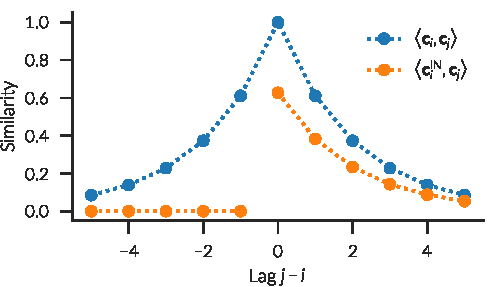
\includegraphics{figures/ctxsim}
    \caption{Similarity of the context to itself $\langle \ctx_i, \ctx_j \rangle$ and to the retrieved context $\langle \ctxin_i, \ctx_j \rangle$ for different lags $j-i$.}\label{fig:ctxsim}
\end{figure}

Finally, the associations from items to context $\mtf$ need to be updated, so that a recalled item can be used to update and partially restore a previous context to retrieve further items.
In the original TCM, this update is given by
\begin{align}
    \mft_{i+1} &= \mft_i \tilde{\mat{P}}_{\tcmitem_i} + a_i \mft_i \mat{P}_{\tcmitem_i} + b_i \ctx_i \tcmitem_i\Tr \\
    a_i &= \gamma b_i \\
    b_i &= \frac{1}{\gamma^2 + 2 \gamma \left\langle\ctxin, \ctx_i\right\rangle + 1}
\end{align}
with projection operators $\mat{P}_{\vc v} = \vc v \vc v\Tr\!/ \norm{\vc v}^2$, $\tilde{\mat{P}}_{\vc v} = \imat - \mat{P}_{\vc v}$, and a free parameter $\gamma$ specifying the relative contribution of previously associated context $\ctxin_i$ and new context $\ctx_i$.
Again, to facilitate the neural implementation, the exact weighting of $\ctxin_i$ and $\ctx_i$ is relaxed while still achieving a good match to data.
Instead of splitting $\mft_i$ into components parallel and orthogonal to $\tcmitem_i$, $\ctx_i\tcmitem_i\Tr$ is added directly into the matrix with a fixed parameter $b$,
\begin{equation}
    \mft_{i+1} = \mft_i + b \ctx_i\tcmitem_i\Tr\text{.}
\end{equation}

Given a context $\ctx$, a mixture of associated items can be recalled as $\tcmitemin = \mtf \ctx$.
To retrieve a single item some form of cleanup has to performed.
Once such a single item has been recalled, the item can be used to recall the associated context as $\mft \tcmitemin$ which in turn can be used to update the current context according to \cref{eqn:ctx-update}.
The updated context allows recalling further items (\cref{fig:tcm}b).

Different cleanup strategies for the recalled item vector can be used.
In the original TCM model, a set of activities $a_i = \tcmitem_i\Tr \tcmitemin$ was obtained and used to make a probabilistic decision according to Luce's choice rule.
The probability of retrieving item $\tcmitem_i$ is given as
\begin{equation}
    P\bigl(\tcmitem_i \bigl|\,\tcmitemin\bigr) = \frac{\exp\!\del{\frac{2a_i}{\tau}}}{\sum_j \exp\!\del{\frac{2a_j}{\tau}}}
\end{equation}
with a parameter $\tau$ that specifies the sensitivity to the activities.

The version of the TCM model presented by \textcite{Sederberg2008}, uses a winner-take-all process based on the leaky, competing accumulator model \parencite{Usher2001}.
In this model, for each possible item a leaky integrator integrates evidence over time.
At the same time, the integrators inhibit each other laterally.
The dynamics can be described by
\begin{equation}
    \vc x_s = \vc x_{s - 1} + \frac{1}{\tau} \del{\vc u - \kappa \vc x_{s - 1} - \lambda \mat L \vc x_{s - 1}} + \vc\eta
\end{equation}
where $\vc u$ is the scaled vector of inputs determined from $\mtf \ctx$ with the current context, $\kappa$ the leak rate, $\lambda$ the lateral inhibition, ${[\mat L]}_{ij} = 1 - \krond_{ij}$ the lateral inhibition matrix, and $\vc\eta$ normal distributed random noise.
This is a more detailed description of how the brain might actually decide for a single item.
However, it is problematic to incorporate within a larger scale neural model under noisy conditions as detailed in \cref{sec:recall}.
For this reason, a different winner-take-all process described in that chapter is used.


\section{Neural context update}\label{sec:ctx-update}
A neural implementation of the TCM needs to implement the updating of the $\mft$ and $\mtf$ matrices discussed in \cref{sec:aml}, the recall of items discussed in \cref{sec:recall}, and updating of the context given by \cref{eqn:ctx-update}, discussed in the remainder of this chapter.
Despite being a simple equation, a number of different implementation approaches are potentially viable.
However, only one of these methods was successful in matching the human data when incorporated into the complete model.
It is still instructive to compare these different approaches and consider why they fail.

\subsection{Boundend integrator}
\Cref{eqn:ctx-update} assumes discrete steps, but for a neural implementation a continuous formulation is more natural and given by
\begin{equation}
    \od{\ctx}{t} = \big(\bar{\theta} - 1\big) \ctx + \bar{\tcmbeta} \ctxin\,\text{.}
\end{equation}
This equation is easily implemented with a neural integrator for a constant $\bar{\theta}$ and $\bar{\tcmbeta}$.
However, there is no limit on the integration of $\ctxin$ anymore so that the proportion of $\ctxin$ added into $\ctx$ can exceed $\tcmbeta$.
To add at most $\tcmbeta \ctxin$ to the context $\ctx$, we can gate the input to the integrator and add a network computing the dot product between $\ctx$ and $\ctxin$.
After thresholding the dot product at $\tcmbeta$, it can be used to suppress the input by inhibiting the gate ensembles (see \cref{fig:ctx-bounded-integrator}).
\begin{figure}
    \centering
    \begin{tikzpicture}[nef]
        \graph [branch down=2.4cm] {
            in/\ctxin [ext] -!- {
                gate/ [ea] -> ["$\bar{\tcmbeta}$"] integrator/\ctx [ea] -> out/ [ext],
                threshold/ [rect] -!- downscale/$\ctx_{\downarrow}$ [ea] -!- length/ [rect],
                dot [net]
            },
            in -> gate,
            in -> dot -> threshold -> [inhibit, "$\Heavi(x - \tcmbeta)$" {rotate=90}] gate,
            integrator -> dot,
            integrator -> [recurrent, "$\bar{\theta}$" above] integrator,
            integrator -> [bend right, out=340] downscale -> [bend right, "$\zeta$" {xshift=-2mm}] integrator,
            integrator -> ["$1 - \norm{\ctx}$" {anchor=south west}] length -> [inhibit] downscale
        };
    \end{tikzpicture}
    \caption{Bounded integrator network.}\label{fig:ctx-bounded-integrator}
\end{figure}
Furthermore, in the original TCM $\ctx$ was kept at unit length while the integration has no such bound.
To keep the unit length, we can project $\ctx$ to another population $\ctx_{\downarrow}$ which projects back to the integrator with a transform of $\zeta = -0.1$.
Picking a $\zeta$ closer to zero allows the $\vc c$ vector exceed unit length by a larger amount while the integrator receives input and will increase the time required to settle back to unit length, whereas a large magnitude of $\zeta$ can lead to oscillatory behaviour.
The $\ctx_{\downarrow}$ population needs to be controlled to only provide the inhibitory input to the integrator as long as $\lVert\ctx\rVert > 1$.
This is achieved by decoding the length of $\vc c$ from the integrator and thresholding it at $1$.
As long as the threshold is not exceeded $\ctx_{\downarrow}$ is inhibited.

To investigate the behaviour of the network, it was fed with new context vectors $\ctxin$ at rate of one vector per second.
These vectors were either orthogonal or had a cosine similarity of \num{0.6} between successive pairs.
\Cref{fig:bounded-integrator} shows the mean similarity of the context vector to itself with given time lag.
\begin{figure}
    \centering
    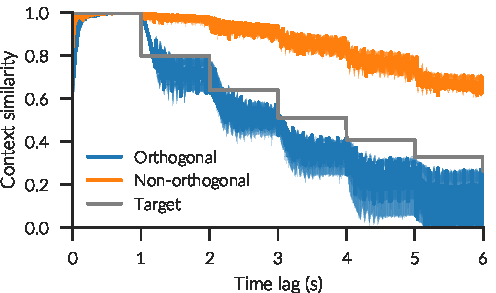
\includegraphics{figures/context-analysis/bounded-integrator}
    \caption[Decay in context similarity with the bounded integrator network.]{
        Decay in context similarity with the bounded integrator network given almost orthogonal inputs and inputs with a similarity of approximately \num{0.6}.
        The desired similarity is given by the gray line. Shaded regions indicate \SI{95}{\percent} confidence intervals.}\label{fig:bounded-integrator}
\end{figure}
For (almost) orthogonal vectors $\ctxin$, the similarity between the context vectors is close under the target.
For non-orthogonal vectors with $\big\langle\ctxin_i, \ctxin_{i+1}\big\rangle \approx 0.6$, however, the similarity of the context vectors is by far larger than the target.
This is caused by the input already being similar to the context and thus stopping the update too early.
Note that it is not sufficient to simply adjust $\tcmbeta$ as depending on the similarity of the inputs it needs to either be incremented or decremented.

\subsection{Alternating update of two memories}
With a single integrator, we have to rely on the dot product between the input vector and current context as a measure of $\tcmbeta$.
This dot product is biased in different directions if the input vectors have differing similarities.
To circumvent this, we need to use two gated memory populations that are updated in alternating fashion.
Then the output of the old context and input vector can be combined according to $\theta \ctx + \tcmbeta \ctxin$ and fed into to the memory buffer for the current context.
The completion of that memory update can be detected by the dot product of the updated context and the current context crossing a threshold of one.
Such a network is shown in \cref{fig:ctx-alt-update}.
\begin{figure}
    \centering
    \begin{tikzpicture}[nef, x=2cm, y=2cm]
        \graph [no placement] {
            in/\ctxin [ext, at={(0,0)}] -> ["$\tcmbeta$"] new/ [pnode, at={(1,0)}] -> cgate/ [ea, at={(2, 1)}] -> current/\ctx [ea, at={(3, 1)}] -> oldgate/ [ea, at={(3, -1)}] -> old/$\ctx'$ [ea, at={(2, -1)}] -> ["$\theta$"] new,
            current -> [bend right, "$-1$"] cgate,
            new -> [out=0, in=225] dot [net, at={(4, 1)}], current -> dot [net],
            dot -> rectification/ [rect, at={(4.5, 0.5)}] -> ["$\Heavi(x)$" anchor=west] heavi/ [pnode, at={(4.5, -0.5)}] -> [inhibit, bend left] cgate,
            heavi -> [inhibit] invert/ [ens, at={(4, -1)}] -> [inhibit] oldgate,
            bias/"$1$" [ext, at={(4.5, -1)}] -> invert,
            old -> [bend right, "$-1$" below] oldgate
        };
    \end{tikzpicture}
    \caption{Alternating update of memory buffers.}\label{fig:ctx-alt-update}
\end{figure}

Unfortunately, this still does not work for non-orthogonal input vectors (\cref{fig:amb}).
In that case the dot product of the updated context and current context are already quite high and the updated context is not completely loaded into the current memory buffer.
\begin{figure}
    \centering
    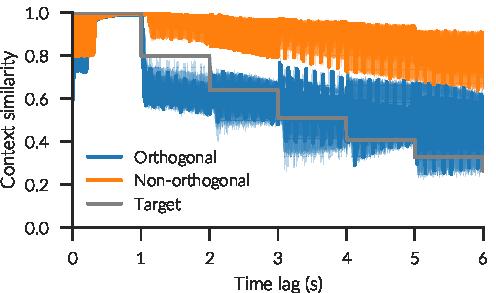
\includegraphics{figures/context-analysis/amb}
    \caption[Decay in context similarity with the alternating update of two memories.]{
        Decay in context similarity with the alternating update of two memories given almost orthogonal inputs and inputs with a similarity of approximately \num{0.6}.
        The desired similarity is given by the gray line. Shaded regions indicate \SI{95}{\percent} confidence intervals.}\label{fig:amb}
\end{figure}


\subsection{Externally controlled alternating memory buffers}
All approaches to determine required context updates based on vector similarity will fail because the similarity of $\ctxin_i$ and $\ctx_{i-1}$ is not known beforehand and can vary widely depending on what contexts are recalled.
Thus, for a properly working context update in the TCM model, the update process has to be controlled by an external control signal (see \cref{sec:control}).
This control signal indicates when the context signal needs to be updated with the provided input and when it has to be kept stable.
If we take the alternating memory buffer network, but control the updating externally (\cref{fig:ctx-ext-ctrl}), it works for both orthogonal and similar input vectors (\cref{fig:ext-amb}).
\begin{figure}
    \centering
    \begin{tikzpicture}[nef, x=2cm, y=2cm]
        \graph [no placement] {
            in/\ctxin [ext, at={(0,0.5)}] -> ["$\tcmbeta$"] new/ [pnode, at={(1,0.5)}] -> cgate/ [ea, at={(2, 1)}] -> current/\ctx [ea, at={(3,1)}] -> oldgate/ [ea, at={(3, -1)}] -> old/$\ctx'$ [ea, at={(2, -1)}] -> ["$\theta$" {very near start, below}] new,
            current -> [bend right, "$-1$"] cgate,
            keep/"keep context" [ext, at={(0,-.5)}] -> ctrl/ [pnode, at={(1,-.5)}] -> [inhibit] cgate,
            ctrl -> ["$-1$" near end] invert/ [pnode, at={(2.5, -0.5)}] -> [inhibit] oldgate,
            bias/$1$ [ext, at={(2.5, 0)}] -> invert,
            old -> [bend right, "$-1$" below] oldgate
        };
    \end{tikzpicture}
    \caption{Alternating update of memory buffers with external control.}\label{fig:ctx-ext-ctrl}
\end{figure}
\begin{figure}
    \centering
    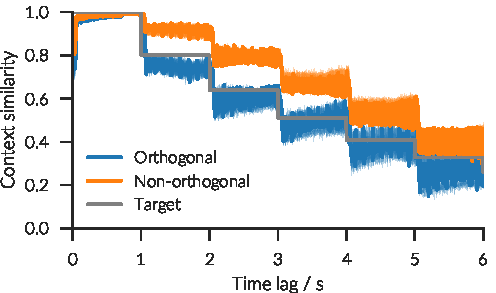
\includegraphics{figures/context-analysis/ext-amb}
    \caption[Decay in context similarity with the alternating update of two memories and external control.]{
        Decay in context similarity with the alternating update of two memories and external control given almost orthogonal inputs and inputs with a similarity of approximately \num{0.6}.
        The desired similarity is given by the gray line. Shaded regions indicate \SI{95}{\percent} confidence intervals.}\label{fig:ext-amb}
\end{figure}

This leads to two predictions.
First, the update of the context signal is not directly regulated by the input, but externally controlled.
Second, there are neural populations that start representing the current context in succession: first the updated context $\ctx$ is constructed in one memory population before it is transmitted to a secondary population $\ctx'$ to be available as old context for the next update.

\chapter{Association Matrix Learning}\label{sec:aml}

The TCM requires two association matrices, $\mtf$ and $\mft$, to be updated.
To translate this into neurons, an appropriate learning rule, the association matrix learning rule (AML), has to be derived.
The TCM gives the update of such an association matrix as
\begin{align}
    \mat M_{i+1} &= \mat M_i + \Delta \mat M_i \\
    \Delta \mat M_i &= \vc v_i \vc u_i\Tr
\end{align}
for adding an association from $\vc u_i$ to $\vc v_i$.
The association matrix after $n$ updates can be expressed as
\begin{equation}
    \mat M_n = \mat M_0 + \sum_{i=1}^{n} \Delta \mat M_i = \mat M_0 + \sum_{i=1}^n \vc v_i \vc u_i\Tr \text{.}
\end{equation}
This allows us to express the neural connection weights after learning $n$ associations as
\begin{equation}
    \weights = \menc \mat M_n \mdec = \menc \mat M_0 \mdec + \menc \sum_{i=1}^n \vc v_i \vc u_i\Tr \mdec
\end{equation}
where $\menc$ is the post-synaptic encoder matrix and $\mdec$ are the pre-synaptic decoders of the identity function.
This equation gives us some important information on how the learning of such association matrices can be implemented.
First, preexisting weights can be implemented as a transform on a normal neural connection that is kept constant.
Second, all the weight changes can be collapsed into decoder changes.
Thus, we need the AML to implement the decoder change given by
\begin{align}
    \tilde{\mdec}_{i+1} &= \tilde{\mdec}_i + \Delta \tilde{\mdec}_i \\
    \Delta \tilde{\mdec}_i &= \vc v_i \vc u_i\Tr \mdec
\end{align}
where $\tilde{\mdec}$ is the matrix of learned decoders.

To implement this within a neural network, the discrete equation has to be converted into continuous form:
\begin{equation}
    \od{\tilde{\mat D}}{t} = \eta \vc v(t) \vc u(t)\!\Tr \mat D \label{eqn:aml}
\end{equation}
with learning rate $\eta$.
Note that while in the discrete formulation all associations are added in with the same strength, in the continuous formulation, the associative strength depends on the learning rate and presentation time.
This equation can be directly implemented with the NEF and thus realized with spiking neurons.
That alone, however, does not ensure the biological plausibility, as any mathematical formulation of synaptic weight changes could be implemented with the NEF\@.
There are also multiple ways to implement the equation with the NEF that have different implications about a potential biological realization.
In the following, several of these possibilities are discussed.


\section{Explicit calculation of weight change}
Both the cue $\vc u(t)$ and target $\vc v(t)$ are available as neural signals.
That allows the implementation of the calculation of the outer product $\vc v(t) \vc u(t)\!\Tr$ in a set of neural ensembles.
The multiplication of each pair of scalars can be accurately implemented in spiking neurons as demonstrated by \textcite{gosmann2015-1}.
Those ensembles can then be connected up to modulate the synaptic strengths from the pre- to the post-populations (see \cref{fig:aml-explicit}) by forming the transpose of the outer product, applying a transform of $\mdec\Tr\!$, and transposing back.
\begin{figure}
    \centering
    \begin{tikzpicture}[nef]
        \graph[no placement] {
            u/$\vc u$ [ext, at={(0, 0)}],
            v/$\vc v$ [ext, at={(2, 0)}],
            uv/$\vc v \vc u\Tr$ [net, at={(1, -1)}],
            u -> uv, v -> uv,
            pre [ens, at={(-1, -3)}, minimum size=30] -- mod/"" [minimum size=0, inner sep=0, at={(1, -3)}] -> post [ens, at={(3, -3)}, minimum size=30],
            uv -> [modulatory, "$\mdec\Tr$" right] mod,
        };
    \end{tikzpicture}
    \caption{Explicit neural calculation of the AML weight change.}\label{fig:aml-explicit}
\end{figure}

It might be surprising that the change in the connection weights between the pre- and post-ensemble does not depend on their own activity, but is controlled externally.
While this is different from many other common learning rules, there is evidence of such heterosynaptic learning in the brain and specifically the hippocampus \parencite{huilme2014,rebola2017,uchida2012}.
Furthermore, this learning rule requires some preexisting structure and connection weights to calculate the signal for the weight modulation.
But as most NEF models do not give a developmental account of how such structures come about, I put this question aside and leave it at something that has to be answered in the future and concerns any type of NEF model, not just this learning rule.
However, there is one more aspect that can be criticized as being biologically implausible: the connections from the outer product calculation depend on the decoders of the pre-population.
It is not clear how the pre-population could transmit this information to this other place.

A similar problem of biological plausibility occurs in classical neural networks and deep learning with back propagation, where the weights for the transmission of the error signal need to be symmetric to the forward weights.
Recently, this concern of biological plausibility in deep learning has been slightly alleviated by the discovery that the weight symmetry is not strictly required.
It is possible for the network to adjust its forward weights to account for existing, non-symmetric backward weights, a process known as feedback alignment \parencite{lillicrap2016}.
Unfortunately, it is not clear whether this can be applied to the situation here.


\section{Explicit calculation of weight change without weight symmetry}
By reformulating $\vc v(t) \vc u(t)\!\Tr \mdec$ as $\vc v(t)[\mdec\Tr \vc u(t)]\Tr$ it is possible to implement the learning rule without the need for a connection to be based on decoders of a neural ensemble it is not related to.
Again there is a set of neural ensembles calculating an outer product (see \cref{fig:aml-explicit-no-sym}).
\begin{figure}
    \centering
    \begin{tikzpicture}[nef]
        \graph[no placement] {
            v/$\vc v$ [ext, at={(2, 0)}],
            uv/$\vc v (\mdec\Tr \vc u)\!\Tr$ [net, at={(1, -1)}],
            v -> uv,
            pre [ens, at={(-1, -3)}, minimum size=30] -- mod/"" [minimum size=0, inner sep=0, at={(1, -3)}] -> post [ens, at={(3, -3)}, minimum size=30],
            pre -> ["$\mdec\Tr$"] uv,
            uv -> [modulatory] mod,
            u/$\vc u$ [ext, at={(-3, -3)}] -> pre,
        };
    \end{tikzpicture}
    \caption{Explicit neural calculation of the AML weight change avoiding weight sharing.}\label{fig:aml-explicit-no-sym}
\end{figure}
But in contrast to the previous approach, if the pre-ensemble is also used as the cue input $\vc u(t)$, the transform $\mdec\Tr$ applied to $\vc u(t)$ is based on that ensemble's decoders decoding $\vc u(t)$.
The transform could even be rolled into the decoder matrix
\begin{equation}
    \mdec_{*} = \mdec\Tr \mdec \text{.}
\end{equation}
As we generally assume, in the context of the NEF, that there is some mechanism in place to establish the decoders to compute arbitrary given functions, this might already be considered a satisfactory answer to the biological plausibility.

However, it is not possible to state the function to obtain the decoders $\mdec_*$ because the function itself depends on the encoding by the neurons.
Moreover, $\mdec_*$ is a symmetric matrix, which is a constraint not respected by the normal decoder optimization process.
But in the context of the NEF, it can be assumed that the neural network can decode the identity function, i.e., there is a connection with decoders $\mdec$.
This can be used to learn a connection with decoders $\mdec_*$.

Given the vector of neural activities $\vc \act$ at time $t$, we have $\vc x = \mdec \vc \act$ and can state
\begin{equation}
    \vc x\Tr \vc x = \vc \act\Tr \mdec\Tr \mdec \vc\act \overset{!}{=} \vc\act\Tr\mdec_*\vc\act \text{.}
\end{equation}
This gives us an error expression as
\begin{equation}
    \err^2(\vc\act) = \left\lvert\vc x\Tr \vc x - \vc\act\Tr \mdec_* \vc\act\right\rvert^2 \overset{!}{=} 0
\end{equation}
with the gradient defined as
\begin{equation}
    \pd{\err^2(\vc\act)}{\mdec_*} = 2 \del{\vc\act\Tr \mdec_* \vc\act - \vc x\Tr \vc x} \del{\vc\act \vc\act\Tr} \text{.}
\end{equation}
The gradient can be used for a weight update rule
\begin{equation}
    \od{\mdec_*}{t} = -\eta_* \pd{\err^2(\vc\act)}{\mdec_*}
\end{equation}
in a (spiking) neural network to perform stochastic gradient descent.

To demonstrate that this learning rule allows the learning of the desired symmetric matrix, it was applied to a connection where the pre-synaptic ensemble was fed with a randomly varying vector signal.
The vector was generated from bandwidth limited Gaussian white noise (upper limit \SI{40}{\hertz}) for each component, normalized, and then multiplied by a bandwidth limited white noise scalar.
The learning rate was set to $\eta_* = \SI{1e-13}{\second^{-1}}$.
We can see that the Frobenius norm of the difference between the learned matrix $\mdec_*$ and the desired matrix $\mdec\Tr\mdec$ continuously decreases (\cref{fig:aml:grad-err}).
The decoded output for some dimensions quickly aligns with the target output (\cref{fig:aml:grad-decode}), but that does not happen for all dimensions.
This might be due to the random input not sufficiently covering the representational space.
\begin{figure}
    \centering
    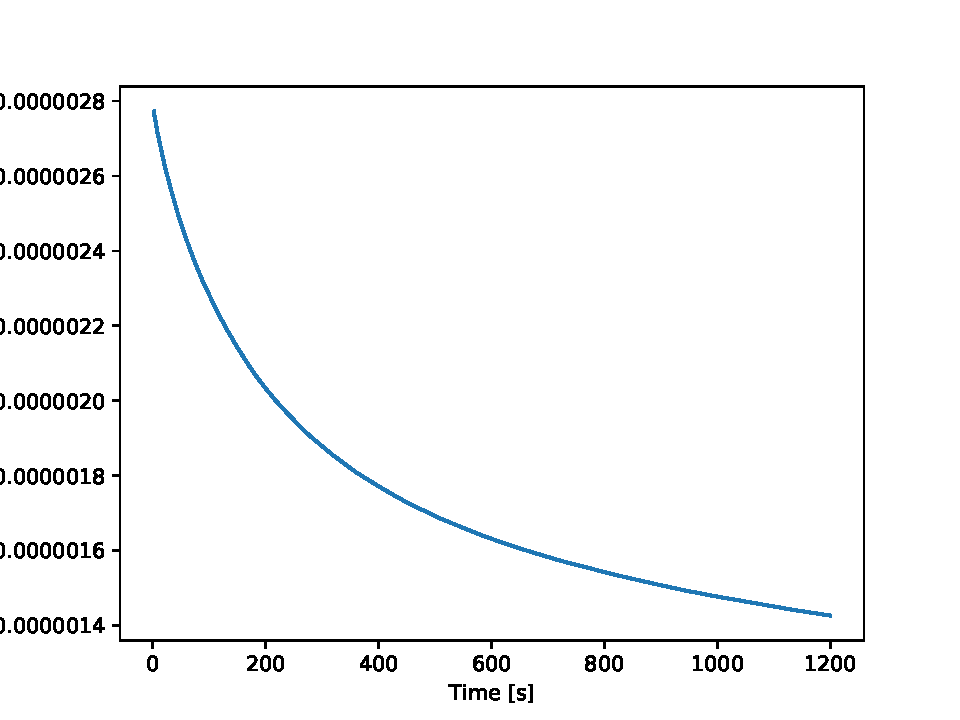
\includegraphics{figures/aml-grad-err}
    \caption{Error $\lVert \mdec\Tr\mdec - \mdec_*\rVert$.}\label{fig:aml:grad-err}
\end{figure}
\begin{figure}
    \centering
    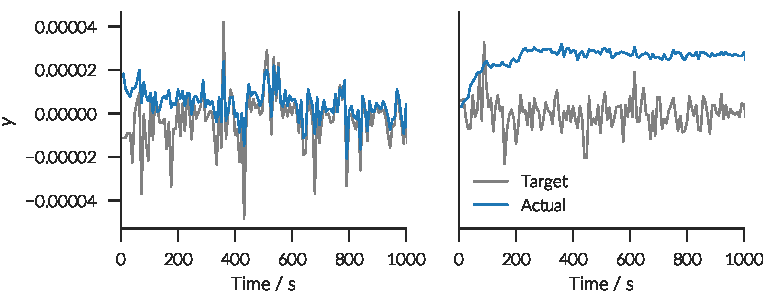
\includegraphics{figures/aml-decode}
    \caption[Example of two outputs decoded with the symmetric weights being learned.]{Example of two outputs decoded with the symmetric weights being learned. The output dimensions on the left quickly aligns with the target, while this does not happen (within the shown time frame) for the output dimension on the right.}\label{fig:aml:grad-decode}
\end{figure}

Again, the pure derivation of a learning rule does not ensure its biological plausibility.
Thus, let us consider the individual terms in the gradient.
The term $\vc\act\Tr \mdec_* \vc\act$ is using the current decoders to decode the ensemble's activity in no way different than usually done in the NEF where the existence of these standard decoders is generally assumed.
The decoded value is then correlated with the ensemble's activity.
The plausibility of this is somewhat unclear to the direct interaction of decoded values and neural activities, but to my knowledge there is no data excluding this possibility.
In particular, the decoded value and activities could be projected to another neural ensembles (see \cref{fig:aml-grad-desc}) that calculates the inner product.
The same, a projection to neural ensemble calculating the inner product, could happen with the decoded value $\vc x$.
Alternatively, $\vc x\Tr \vc x$ could directly be decoded (as a square of the individual components all projecting into the same dimension).
\Cref{fig:aml:neural-grad-err} shows the time course of the error when learning $\mdec_*$ with such a neural gradient computation.
The observed decrease demonstrates the basic viability of this approach, but the learning is slower and flattens out earlier due to the spiking noise.
\begin{figure}
    \centering
    \begin{tikzpicture}[nef]
        \graph[no placement] {
            pre [ens, at={(0, 0)}, minimum size=30] -- mod/"" [inner sep=0, minimum size=0, at={(2.5, 0)}] -> post [ens, at={(4, 0)}, minimum size=30],
            pre -> [bend left] act/"$\vc\act\Tr \mdec_* \vc\act$" [net, at={(0, 3)}],
            pre -> [bend right, "$\mdec_*$" xshift=-3mm] act,
            pre -> targetact/"$\vc x\Tr \vc x$" [net, at={(1.5, 1.5)}],
            act -> combine/"" [pnode, at={(3, 3)}],
            targetact -> ["$-1$"] combine,
            combine -> [modulatory, out=270, in=90] mod,
        };
    \end{tikzpicture}
    \caption{Neural computation of the error signal necessary for learning symmetric decoders with gradient descent.}\label{fig:aml-grad-desc}
\end{figure}
\begin{figure}
    \centering
    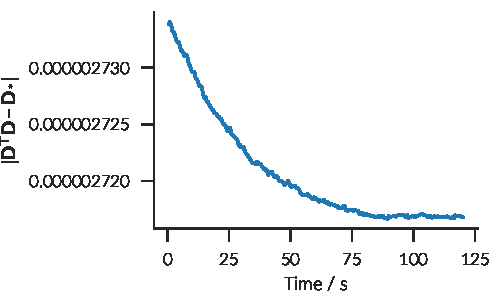
\includegraphics{figures/aml-neural-grad-err}
    \caption{Error $\lVert \mdec\Tr\mdec - \mdec_*\rVert$ with neural gradient calculation.}\label{fig:aml:neural-grad-err}
\end{figure}


The whole term $\vc\act\Tr \mdec_* \vc\act - \vc x\Tr \vc x$ is a scalar that influences all synapses.
This could be realized by a broadly acting neuro-modulator or by extensive connectivity of the neural ensembles calculating this error term.
Neither option is implausible.
This gradient term seems to play a role in weight normalization as it acts equally on all weights and the magnitude depends on the magnitude of the values of $\mdec_*$.
Also, without it all weight changes would always be negative.
Note that in many learning rules, normalization factors are often criticized as implausible for requiring knowledge of the whole weight matrix at the level of a single synapse.
This critique does not apply to this learning rule.
The decoding matrix is only used to decode from the activities which require only local knowledge of the weights.

Finally, the term $\vc\act \vc\act\Tr$ correlates neuron activities and appears somewhat Hebbian-like.
Hebbian learning is one of the best studied ways that biological systems learn.
In this form of learning pre- and post-synaptic neurons become connected when they fire in short succession.
In contrast to this usual account, here two pre-synaptic neurons connect to the same post-synaptic neuron if they fire together.
Again, the biological plausibility of this is somewhat uncertain, but cannot be outright rejected.


\section{Implicit error calculation}
The previous two implementations of the AML use minimal assumptions about the computational power of synapses.
All that is needed are additive weight changes proportional to some error signal.
However, it has been proposed that synapses might not simply transmit information, but also perform computations \parencites{abbott2004}[Ch.~5]{koch2004}.
In particular, \textcite{andreasstockel2018} showed that conductance-based synapses can be used in the NEF to compute nonlinear functions like multiplication.
That should allow us to roll the explicit outer product, required in the previous two approaches, into the synapses itself.
This requires considerably fewer neurons as no neural populations are required for each product.

In this thesis, I am using an implementation that corresponds to this implicit error calculation, but implements the required synaptic computation in pure math rather than implementing it with actual synaptic models.
This is mainly to reduce simulation times and is not meant as a statement that this is likely to correspond to the brain's implementation as there is not enough evidence to make such a strong claim.


\section{Normative interpretation}
While the AML cannot be outright rejected as biologically implausible, there are definitely some open questions concerning it.
Nevertheless, it should not be evaluated purely on this fact.
Many models in cognitive science, psychology, and computational neuroscience assume the encoding of associations in an outer product matrix \parencite[e.g.,][]{kajic2017,nowak2001,Brown2000}.
Ultimately, the validity of all those models depends on the possibility that the brain can learn such a matrix.
As such, the AML makes it explicit which operations have to be implemented to enable such learning.
If these turn out as either not being implemented in the brain or as not being implementable at all, it would follow that the brain has to use some other mechanism to represent associations.
Thus, the AML has merit as a normative theory, describing what the brain is ought to do, and directing research to open questions.

That being said, the AML does not make any assumption about the pre-synaptic neurons.
With such assumptions, some of the restrictions of the AML might be lessened.
For example, assuming orthogonal encoders, the decoder matrix $\mdec$ will be orthogonal too.
That in turn means that $\mdec_* = \mdec\Tr \mdec = \imat$ becomes the identity matrix which is independent of the exact decoders.
This simplifies connectivity and removes the need to learn the symmetric matrix $\mdec_*$ which alleviates some of the concerns of biological plausibility.

The dentate gyrus in the hippocampus is often assumed to perform pattern separation, which is a form of orthogonalization.
Hence, it might be possible that the hippocampus learns associations with a form of the AML where $\mdec_*$ ends up being the identity matrix and thus simplifies the learning rule itself.


\section{Properties of the AML}
So far the considerations about the AML were purely theoretical.
\Cref{fig:aml} demonstrates that an implementation of the AML can indeed learn associations in a spiking neural network.
Five different cue-target pairs were presented for one second each, before testing the recall with the same cues, but no target vectors.
The initially presented target vectors are almost perfectly recalled.
Note that no catastrophic forgetting occurred and each association was learned with a single presentation of the cue-target pair (one-shot learning).
Most other learning rules exhibit destructive interference between the items in this scenario.
As an example, \cref{fig:aml} also shows the same experiment using the Prescribed Error Sensitivity (PES) learning rule \parencite{bekolay2013}, which is commonly used in NEF models \parencite[e.g.,][]{komer2015,Rasmussen2017}.
Here all associations except for the last get destroyed.
It is still possible to learn associations with PES, but it requires the presentation of each item multiple times in interleaved fashion, i.e., one-shot learning cannot be done to learn associations in a reliable way.
\begin{figure}
    \centering
    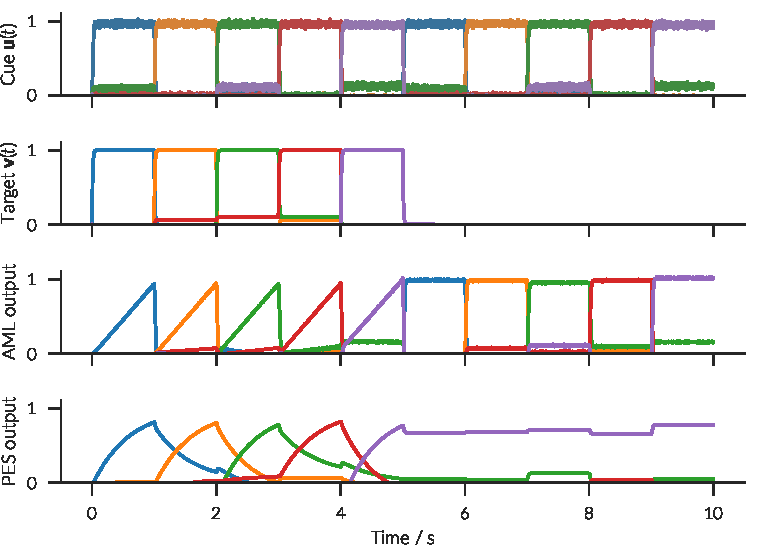
\includegraphics{figures/aml}
    \caption[Learning and recall testing of five cue-target pairs with the AML and PES.]{Learning and recall testing of five cue-target pairs with the AML and PES\@. Each colored trace is the dot product with one of the vectors used. The cue vectors $\vc u(t)$ and target vectors $\vc v(t)$ differ.}\label{fig:aml}
\end{figure}

This ability for one-shot learning with the AML is due to the $\mdec_*$ matrix, which accounts for the interference between neurons.
In fact, the AML and PES are the same except for that matrix.
The PES learning rule can be expressed as
\begin{equation}
    \od{\tilde{\mdec}}{t} = \eta \vc v(t) \vc\act_{\vc u}\Tr(t) \text{,}
\end{equation}
while the AML learning rule can be written as
\begin{equation}
    \od{\tilde{\mdec}}{t} = \eta \vc v(t) \vc u(t)\!\Tr \mdec = \eta \vc v(t) \vc\act_{\vc u}\Tr(t) \mdec\Tr \mdec
\end{equation}
which is the same, except for $\mdec_* = \mdec\Tr \mdec$.

The one-shot learning ability comes with some limitations, though.
The learning rule is restricted to learn transformations that can be expressed as outer product matrices, while learning rules like PES can learn arbitrary transformation matrices.
Moreover, the learning rule is essentially trying to learn a look-up table, mapping items to other items.
Thus, one should not expect the AML to generalize to unseen mappings.

This might be another reason, besides the stability-plasticity dilemma, why a two-stage memory system is needed.
The first stage would learn simple associations with the AML and only in the second step of consolidation with a different learning rule, commonalities get extracted for generalization.
This is consistent with data that shows that generalization improves with sleep.
For example, sleep improves transitive inference \parencite{stickgold2013-2} and gives insight into implicit rules \parencite{wagner2004}.
Experience replay in hippocampus might be responsible for the necessary interleaving of memory traces when using a learning rule that allows for more generalization, but exhibits destructive interference such as PES \parencite{mcclelland1995-1,kumaran2016}.
Overall, it is likely that AML only represents a first step in the association learning process and multiple learning rules are at play here.
That the brain uses no single general purpose learning rule, but combines different learning rules has been forcefully argued by \textcite{gallistel2009}.


\section{AML accounts for neural changes during association learning}\label{sec:aml-neural}
\Textcite{ison2015} reported that individual neurons in hippocampus (and parahippocampal cortex) change their firing rapidly to encode newly learned associations.
They recorded from the medial temporal lobe of \num{14} epilepsy patients that needed to undergo surgery.
They identified neurons that responded to specific visual stimuli of pictures of persons and landmarks and recorded the response to this \emph{preferred} (P) stimulus.
Then the participants learned associations between pairs of a person and a landmark.
Besides multiple tasks to assess the learning, the neuron responses to the different stimuli were recorded again after learning.

Pair-coding units could be identified that showed an elevated firing rate only to the preferred stimulus before learning (BL).
After learning (AL), those same units showed an elevated firing rate only to the preferred and associated non-preferred (NP) stimulus.
This can also be observed for associations learned with the AML\@.
\Cref{fig:aml-net} shows a NEF network that implements the learning of associations between persons and landmarks to reproduce the experiment by \textcite{ison2015}.
The connections weights from both pre-ensembles $\vc l$ and $\vc p$ are initialized with the identity transform.
To achieve firing rates closer to the recorded data, the maximum firing rates of the ensembles were sampled uniformly from \SIrange{10}{20}{\second^{-1}} (instead of \SIrange{200}{400}{\second^{-1}} used in the CUE model) and intercepts were sampled uniformly from \numrange{0.1}{1}.
The dimensionality of the ensembles and semantic pointers was set to \num{32}.
Furthermore, Gaussian white noise with a mean of \num{0.01} and standard deviation of \num{0.05}, low-pass filtered with a time-constant of \SI{0.1}{\second}, was injected into the neurons to account for neural background firing.
The recorded spikes were analyzed analogous to \textcite{ison2015}.
\begin{figure}
    \centering
    \begin{tikzpicture}[nef]
        \graph [no placement] {
            landmark [x=-2, y=0, ext] -> L/"$\vc l$" [x=0, y=0, ens] -- c1/"" [inner sep=0, minimum size=0, x=2, y=-0.5] -> post [x=4, y=-1, ens];
            person [x=-2, y=-2, ext] -> P/"$\vc p$" [x=0, y=-2, ens] -- c2/"" [inner sep=0, minimum size=0, x=2, y=-1.5] -> post;
            L -> err/"" [x=1, y=-1, pnode] -> [bend right, modulatory] c1;
            P -> err -> [bend left, modulatory] c2;
            post -> output/"" [x=6, y=-1, ext];
        };
    \end{tikzpicture}
    \caption[NEF network for associating two stimuli with the AML.]{NEF network for associating two stimuli (persons with landmarks here) with the AML.}\label{fig:aml-net}
\end{figure}

The main results obtained from the experimental and model data are shown in Figs.~\ref{fig:aml-spikes} and~\ref{fig:aml-population-response}.
\begin{figure}
    \centering
    \subcaptionbox{Experimental data}{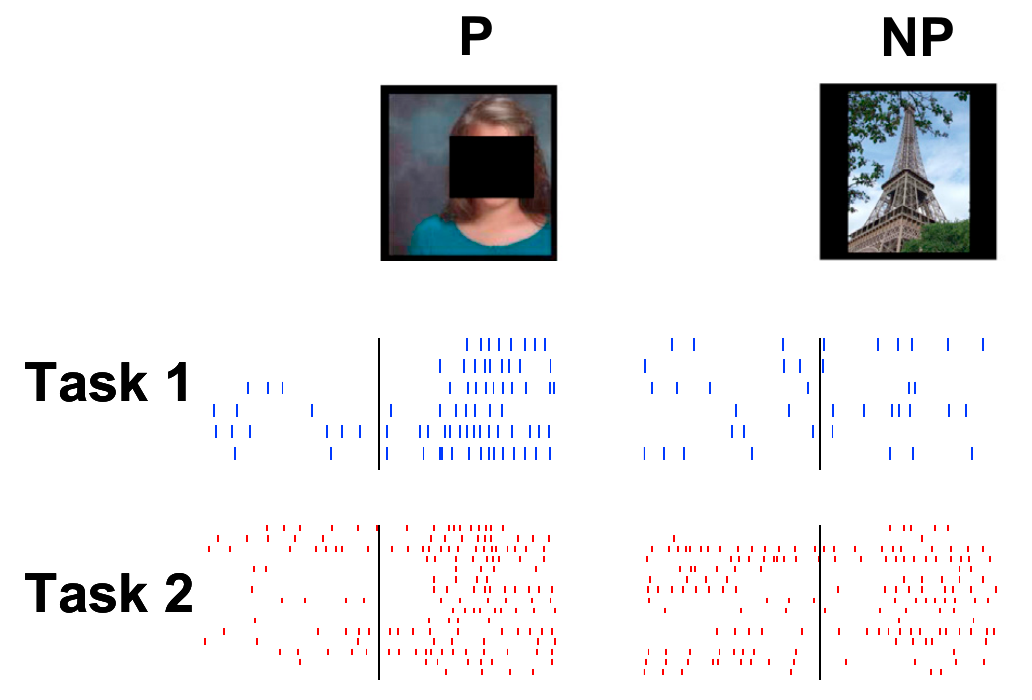
\includegraphics[width=9cm]{figures/ison2015-spikes}}

    \vspace*{0.34cm}
    \subcaptionbox{Model data}{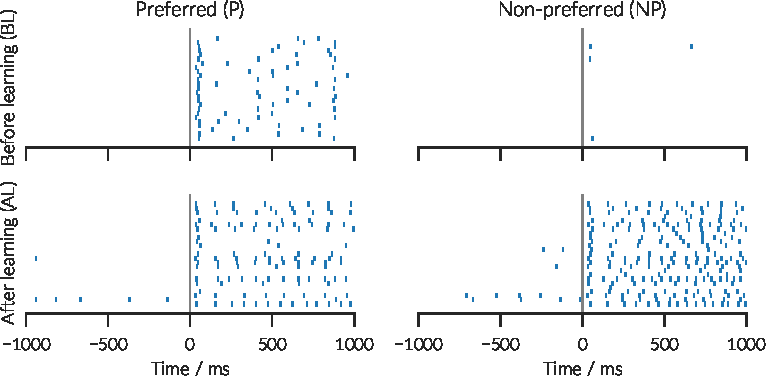
\includegraphics{figures/aml-spikes}}
    \caption[Change in spiking behaviour when learning associations.]{Change in spiking behaviour when learning associations. (a) Exemplary spikes recorded from human hippocampus for the preferred (P) and non-preferred (NP) stimulus. Task 1 (blue) is before, task 2 (red) after learning the P-NP association. The black line marks the stimulus onset. Figure adopted from \textcite{ison2015} under the Creative Commons Attribution 4.0 International license. (b) Spikes recorded from the NEF model learning the P-NP association with the AML\@.}\label{fig:aml-spikes}
\end{figure}
\begin{figure}
    \centering
    \subcaptionbox{Experimental data}{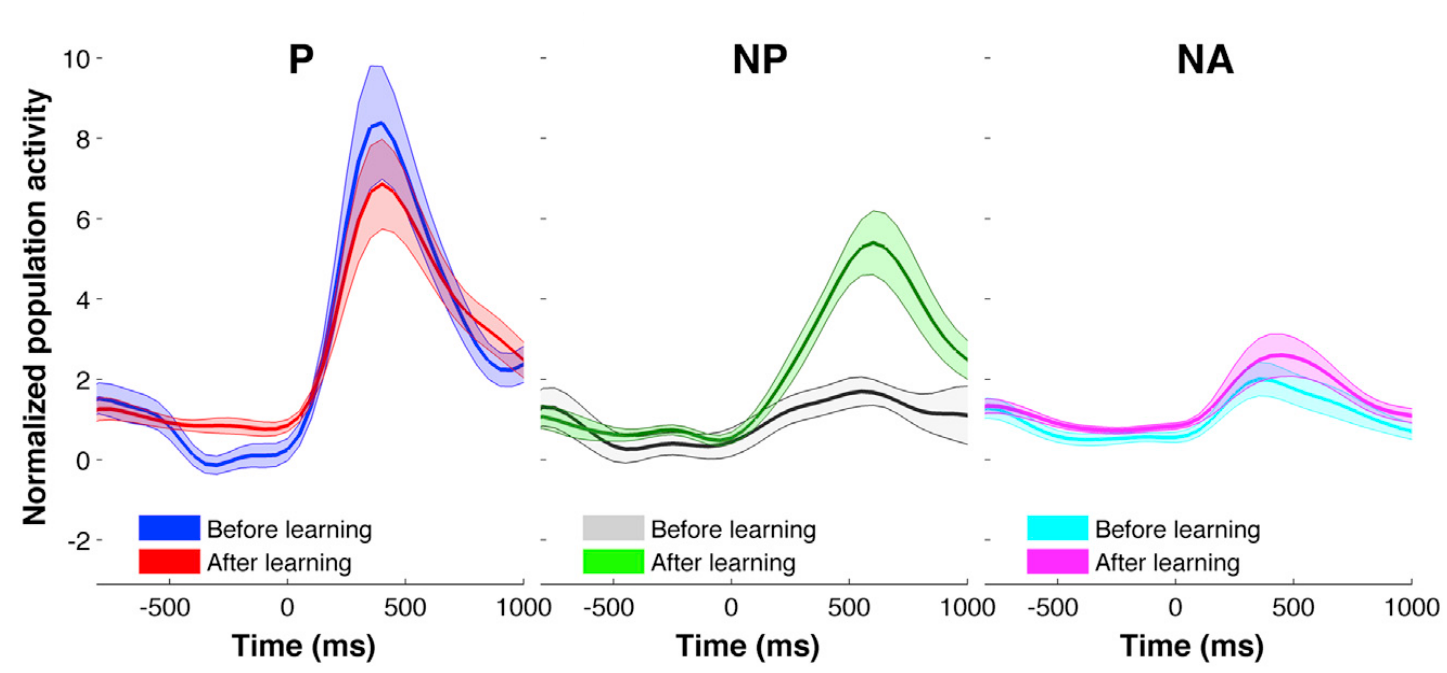
\includegraphics[width=12cm]{figures/ison2015-pop}}

    \vspace*{.75cm}
    \subcaptionbox{Model data}{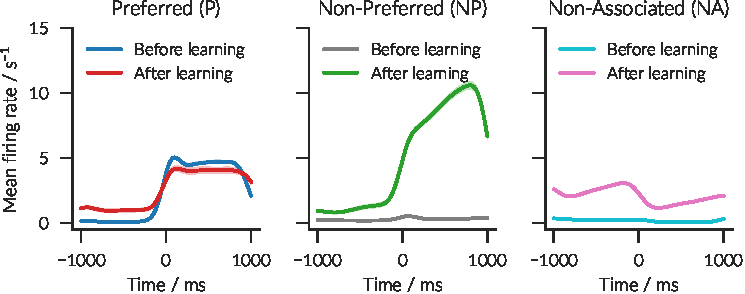
\includegraphics{figures/aml-population-response}}
    \caption[Population response for pair-coding units.]{Population response for pair-coding units to the preferred (P), non-preferred (NP), and non-associated (NA) stimuli before and after learning. Times are relative to stimulus onset. Shaded regions indicate the standard error of mean. (a) Normalized population activity from (a) experimental and (b) model data. Figure (a) adopted from \textcite{ison2015} under the Creative Commons Attribution 4.0 International license.}\label{fig:aml-population-response}
\end{figure}
Pairwise coding units, showing elevated firing in response to the preferred stimulus before learning and the non-preferred stimulus after learning without an increased response to any other stimuli, have been selected.
The normalized population activity in response to the preferred stimulus shows no or only a minimal change with learning in both the experimental and model data.
For the non-preferred stimulus the population activity increases slightly on stimulus onset which is more pronounced in the model data.
This might be explained by the model not including any visual processing that could delay and smooth out that response.
After learning, this population response is increased in both sets of data.
For non-associated stimuli the model shows a minimal decrease in the normalized population activity with learning, while the experimental data shows no significant change.
Overall, the model matches the main aspects of the experimental observations.
A better quantitative fit might be achievable with more careful parameter selection in the model.


\section{Weight normalization}
Note that the AML allows weights to grow without bound.
By introducing a factor of $1 - \vc v(t)\!\Tr \hat{\vc v}(t)$ this can be prevented where $\hat{\vc v}(t)$ is the retrieved, learned association.
But similar to other weight normalizations it introduces the need for each weight to have access to the global population activity and weights as $\hat{\vc v}(t) = \tilde{\mdec} \vc\act_{\vc u}(t)$.
Such global dependencies are often criticized for not being biologically plausible.
As such, I decided to take a slightly different approach with an equivalent effect.
Instead of including the dot product $\vc v(t)\!\Tr \hat{\vc v}(t)$ in the learning rule, it can be computed by another neural population and the thresholded result can be used to inhibit the population providing $\vc v$.
Once fully inhibited, $\vc\act_{\vc v}(t)$ will be all-zero and thus prevent further weight changes.
In the CUE model, the inhibition threshold is adjusted to follow $1 + \exp(-t)$ for learning the $\mtf$ matrix where $t$ is the time since the trial started.
This is intended to account for rehearsal effects that are not explicitly modelled and is analogous to the extended TCM model by \textcite{Sederberg2008}.

\chapter{Recalling items}
In the original TCM model (TODO ref) the activations $a_i$ of items in the memory is mapped to a recall probability by a softmax function
\begin{equation}
    P(\tcmitem_i | \ctx) = \frac{\exp(2a_i/\tau)}{\sum_j \exp(2a_j/\tau)}
\end{equation}
with a free parameter $\tau$ controlling for the sensitivity.
While this does well in capturing the recall probabilities, it does not provide much insight in how this recall process might be realized neurally.
In an extension of the TCM model (TODO ref) a winner-take-all (WTA) process based on the widely-used leaky, competing accumulator (LCA) model by TODO ref was used.
This works well if the output can be evaluated in a mathematical analysis.
However, within the CUE model other parts of the model need to recognize when a single recall is completed to update the context and reset the recall system.
As I will show, this is difficult to do robustly with the LCA model, but more easily with an alternate WTA mechanism termed the independent accumulator (IA) model.
A comparison of these two networks has also been previously published as TODO ref.


\section{Leaky, competing accumulator model}
Given $D$ choices, the leaky, competing accumulator (LCA) model proposed by TODO ref describes the dynamics of $D$ scalar state variables $x_i(t), 1 \leq i \leq D$ as
\begin{equation}
    \od{x_i}{t} = \frac{1}{\tau} \del{u_i(t) -\kappa x_i - \lambda \sum_{j \neq i} x_j}, \quad x_i \geq 0 \label{eqn:lca}
\end{equation}
where $u_i(t)$ are the external inputs, $\kappa$ is the leak rate, $\lambda$ the lateral inhibition, and $\tau$ the integration time-constant.
Each state variable $x_i$ is kept non-negative by setting negative values to 0.
Intuitively, each state variable integrates its input with leak term of $-\kappa x_i$ and provides lateral inhibition to all other state variables.
Given one input $u_i > u_j$ for all $j \neq i$, the state variable $x_i$ will converge to $u_i$ while all other state variable $x_j, j \neq i$ will converge to $0$ if $\kappa = \lambda = 1$ (TODO appendix).
In the following analysis, $\kappa = \lambda = 1$ will be fixed.
Other choices of $\lambda$ affect the effective integration time-constant $\tau$ and gain on the input, while changing $\beta$ will result in undesired behaviour (TODO ref/appendix).

By means of priniciple 3 of the NEF, the prescribed dynamics can be exactly implemented in the NEF\@.
Here, one ensemble per state variable is used (TODO figure) and the gains and biases of the neurons are distributed as described in TODO to ensure the rectification of the state variables.


\section{Independent accumulator model}
The dynamics of the independent accumulator (IA) model are given by
\begin{align}
    \od{x_i}{t} &= \frac{1}{\tau_1} u_i(t) + \frac{1}{\tau_2} \del{\bar{x}_i - \bar{\lambda} \sum_{j \neq i} \bar{x}_j}, \quad x_i \geq 0 \\
    \bar{x}_i &= \Heavi(x_i - \vartheta)
\end{align}
where $u_i(t)$ again gives the external input, $\tau_1$ and $\tau_2$ are feedforward and feedback time-constants, $\bar{\lambda}$ is an inhibition constant, $\Heavi$ is the Heaviside step function, and $\vartheta$ is a threshold.
The Heaviside non-linearity is the crucial difference to the LCA model as we can reduce this equation to \cref{eqn:lca} by setting $\tau = \tau_1$, $k = -\tau_1/\tau_2$, and $\lambda = \bar{\lambda} \tau_1/\tau_2$ when not considering the Heaviside function.
Through the Heaviside function, the accumulators will act as perfect (opposed to leaky) and independent integrators.
Only when the threshold $\vartheta$ is reached, the winning choice will be stabilized by feedback while all non-winning choices will be inhibited.

These dynamics can again be neurally implemented by means of the NEF\@.
While for the LCA model a single layer was sufficient, it is best to use two layers to implement the IA model.
The first layer consists of independent accumulators representing the state variables $x_i$.
This layer projects to the second layer that performs the computation of $\bar{x}_i$ (i.e.\ the Heaviside function).
The second layer projects back to first layer and can be used to read out the output of the network.

\section{Comparisons of the WTA networks}
The pure analytical description does not tell which network is better suited for certain tasks.
To compare these networks, I simulate them with an input of $u_i = u - s\del{1 - \krond_{1i}} + \eta_i$, where $u$ is the magnitude of the largest input, $s > 0$ is the target separation, $\krond$ is the Kronecker delta, and $\eta_i$ is Gaussian white noise with a standard deviation of $\sigma$.
Here, without loss of generality as we can reorder the indices, the first input is always set to be the target and all other inputs are set to be lower by $s$.
The rationale behind this is that it should present the hardest case because every is close to the largest input.
As $s \rightarrow 0$, the problem will get more difficult as the separation of the target shrinks.
Note, that $u$ determines the general baseline of inputs in addition to the value of the largest input.
Furthermore, it is important to consider the influence of noise $\eta_i$ on the robustness of the decision process.

As the input lists to the CUE model will be about 10 to 12 items, I compare the networks $d=10$ choices.
To make a fair comparison 200 LIF neurons are used per choice in either model.
In the IA model this means, that the number of neurons is split between the first and second layer.
Here I use 150 neurons in the first, and 50 neurons in the second layer.
As the first layer is performing the evidence accumulation it needs to more accurate and requires more neural resources.
Due to the lower number of neurons in the output layer, the decoded output has a higher variance.
This, however, is not as relevant as the variance in interpreting the output.
If all other choices do not produce an output, the winning choice can still be clearly identified despite the variance.

Given this basic setup of the comparison, a number of metrics give insight in the performance of the networks.
First, we want the network to reach a \emph{clear decision} which I define as exactly one output being above a threshold of \num{0.15} during the time interval from \SIrange{1}{2}{\second} simulation time while all other outputs remain below the threshold.
The threshold of \num{0.15} was chosen as it is usually sufficient to tell a zero and non-zero signal apart despite spiking noise (except for very low neuron numbers or firing rates).
This metric requires that the output does not change during the interval as this might cause problems in downstream networks that operate on the output.
Also, with a change in output it would be unclear which output should be taken as the actual decision.
One thing this metric does not take into account is whether the output corresponds to the highest input.
This, whether a decision is \emph{correct}, is the second metric.
But note, that in some situations within larger scale network a wrong, but clear decision, can be preferable to a decision that tends to be correct, but is unstable.

Two more metrics are used for all trials that reached a clear decision.
The amount of time taken to fulfill the conditions for a clear decision are considered as the \emph{decision time}.
It measures how fast the network is obtaining the decision.
Finally, the networks can produce transient outputs unrelated to the final decision.
A downstream network might consider this output as an actual decision and thus those transient outputs should be as small as possible.
The \emph{highest output of a losing choice} during the whole simulation is taken as a metric for this.


\subsection{Results}
Figure~TODO shows the proportion of trials that the LCA network reaches a clear decision for different input parameters.
The input magnitude $u$ must be large enough to reliably exceed the \num{0.15} detection threshold under noise.
For $u = 0.2$ and even low amounts of noise the network fails to reach a clear decision.
However, it seems that a input magnitude too large decreases performance as well when we compare the performance for $u=0.6$ and $u=1$.
Increasing the noise standard deviation $\sigma$ or decreasing the target separation $s$, both decrease the performance as this makes the problem harder.
Interestingly, the IA network does not fail to reach a clear decision in any of these conditions.

Moving on to correct decisions, the LCA network always produced the correct output given it produced a clear decision.
The IA network, may produce incorrect outputs despite a clear decision (TODO figure).
Again, as the problem gets harder either by decreased target separation or increased noise, the network performance on this metric decreases.
Note that the feedforward integration time-constant can be increased to integrate evidence over a prolonged time period  to increase performance on this metric (right-most panel).

This, however, will increase the decision times.
These tend to be already slower for the IA network than for the LCA network (TODO figure).
Additional noise can shorten the decision times in the IA network as it increases the likelihood of an integrator randomly accumulating enough evidence to cross the threshold.
For the LCA network the noise level only has a minor influence on the decision time and was averaged over in the plot.
In other words, noise in the LCA network influences whether a decision can be reached, but not how long it takes to reach a decision if one is reached.

Finally, both networks might produce a transient response (TODO figure).
This is inherent in the LCA network because the state variables are directly used as output and gets worse with increased noise.
In the IA network, this transient response is caused when two accumulators cross the threshold in close temporal proximity before the inhibition from the first one can silence the remaining accumulators.
By increasing the feedforward time-constant, this transient response gets reduced as the evidence integration gets slowed down and this temporally stretches out when accumulators cross the threshold.


\subsection{Discussion}
Neither network performs better on all metrics.
Thus, each is best suited for a different purpose.
In situations where a continuous adjustment of a decision is necessary, the LCA network will most-likely be the better choice.
Under noisy conditions it is not necessarily able to produce a stable, clear output, but if a clear output was obtained, it was always correct.
If the input changes, the output will adjust according to the networks time constant and allow for continuous updates.
Unfortunately, this also makes the network susceptible to noise.

The IA network will be better for discrete series of decisions.
It does not produce a continuous output, but waits until the evidence integration threshold is crossed at which point the network needs to be inhibited to be reset and obtain another decision.
While this produces sequential and discrete decisions, it has the advantage that evidence can be accumulated over a longer time frame to average out noise.
Depending on the choice of the integration time-constant, the IA network will either be not as quick or as reliable in identifying the correct winner as the LCA network.
However, it will eventually produce a clear decision that a downstream network can act on (as long as at least on input is strictly positive).
This can be important in a larger scale model where stalling a decision indefinitely can result in a breakdown of model behaviour.
Or in other words, sometimes it is better to act on a wrong decision that to not act all.
For example, in memory recall it might be better to produce a wrong output and continue to recall the next item than indefinitely trying to recall an item that cannot be recalled.
It is also worth pointing out that the IA network allows for dynamic control of the decision speed by adjusting the $\vartheta$ threshold through a bias input to the second layer.

As mentioned it is also important to consider the transient outputs of the network within a larger scale model.
Such transient responses are inherent in the LCA model as the state variable is directly used as an output.
One could pass the output through a thresholding layer, but the right choice of threshold is not clear as the output magnitude will depend on the input magnitude.
If the threshold is too low, a transient response would be produced even with the thresholding layer.
If it is too high, small inputs might not produce an output at all.
While the IA can also produce transient responses, these can be reduced to almost zero by a proper selection of the integration time-constant according to the input magnitude and target separation.

By increasing $\tau_1 \rightarrow \infty$, the IA discrimination ability can be increased without bound.
This is sometimes used as argument to criticize these sort of models (TODO ref) because there is no sensible stopping criterion.
However, this does not consider that there might be a cost to come to a decision.
If that cost is included, there is a trade-off between accurate decisions and the cost incurred by taking more time to decide.
Furthermore, this argument also assumes perfect integration accuracy which an actual neural system cannot have due to neural noise and limited neural resources.

To summarize these findings, for the recall of items in memory experiments the IA network is more suited.
Such recall requires discrete decisions and a stable input to downstream motor systems producing the response.
Such a stable input cannot be guaranteed with the LCA network and it provides challenge to detect when a recall is completed.
TODO ref still used the LCA network for modelling the recall, but it is important to highlight that they upon reaching the decision threshold the state variable where immediately set back to zero.
This is easy to do in a pure math model, but when transitioning to a full neural model detecting the decision and resetting the state variables is much more difficult as it cannot be done instantaneous.

Finally, let us consider the biological plausibility briefly.
Both networks where simulated in spiking neurons which ensures a certain degree of biological plausibility.
Also, accumulation of evidence to a threshold is a well known finding for neurons in LIP (TODO ref).
Often this is assumed to be a gradual integration, but when looking at individual trials instead of the trial-average, a distinct step response becomes evident (TODO ref).
This matches the output of the second layer of the IA network.
However, both networks have in integration layer with gradually increasing firing rates which implies that such neurons should exist too.
Ultimately, I also want to highlight that this is not as issue which of these two networks is the \emph{one} network employed in the brain.
It is certainly possible, that the brain employs both networks for different tasks as they have different strengths and weaknesses.


\section{Recall network}
The recall network in the CUE model is based on the independent accumulator network.
Each potentially recallable item is regarded as one choice.
An additional choice is added to represent a failed recall.
This is a stand-in for additional items that might be present in the recall network, but have not occurred in the learned list.
It is also a way of providing a time-limit on trying to recall a particular item and prevents pure noise resulting in a successful recall of one of the learned list items.
The additional choice is fed a constant signal of TODO\@.

TODO noise

Furthermore, the IA network is embedded into further components.
First, items are represented as Semantic Pointers, but the IA network needs a separate utility value for each potential choice.
Thus, the incoming connection uses the matrix collecting the Semantic Pointers of all possible list items as transform, effectively calculating a dot product between the input signal and each potential item.
These utility values are then rectified to only consider positive evidence.
By subtracting TODO OSE threshold from the input utilities provided by the OSE output, the TODO OSE threshold is implemented.

The IA network does not produce an output during the evidence accumulation phase.
It is, however, helpful to have a persistent output of the last recalled item (note that this is still different from the output of the LCA network).
To achieve this, the output of the IA network is routed through a gated memory that is only updated when the IA network produces an output.
As the gated memory stores a Semantic Pointer, a transform matrix needs to be applied to the IA output to project the choice back into the Semantic Pointer space.
The updating is controlled by inhibiting the memory gate by default and disinhibiting it (by inhbiting the inhibitory population) when the IA network produces output.

Repetition errors are rarely made in recall experiments.
Thus, it is necessary to inhibit already recalled items.
However, this inhibition should not happen immediately as otherwise the recall output would be inhibited to quickly for downstream network to act upon.
Thus, a two-stage process is used.
First, an initial working memory population gets immediately updated by feeding in the current recall.
This will add the recalled Semantic Pointer into the representation of items to inhibit.
From that representation and the current recalled item, a dot product is calculated and thresholded add TODO\@.
Once the threshold is crossed the gate to the memory population is inhibited as the new item should be added into the representation, but not completely overwrite it.
The output of that memory population is fed to a gated memory that provides the inhibition to recall state.
The gate for this memory is controlled externally and disinhibited once the downstream processing has completed.
Note that the output of that memory population is projected back into utility values and thresholded to prevent positive evidence from the inhibition memory.

Finally, the recall network needs to be reset if a recall fails to allow to continue trying to recall the item for the next position in serial recall.
Here the proble is, that if the IA output for a failed recall is directly used to inhibit the IA network to reset it, this will also immediately inhibit the output used for the inhibition.
This will not reliably reset the network as the reset signal is disabling itself.
Thus, the signal will be fed to an integrator until a threshold is reached and then the signal of the integrator is used to provide an inhibitory pulse to the IA network.
The slower decay of the integrator ensures a sufficient length of the pulse to restart the recall process.

\chapter{The complete model}

Now we have all the essential components to construct the complete context-unified encoding (CUE) model.
\Cref{fig:general-routing} gives an overview of the information flow between the different components.
The Semantic Pointers $\spv v$ for the presented items are the input to the model and the recalled items $\hat{\spv v}$ of the \pop{item recall} network are the model output.
The part of the model corresponding to the TCM consists mainly of the $\mft$, $\mtf$, and \pop{context} networks, whereas \pop{OSE} and \pop{position} correspond to the OSE\@.
The \pop{position} network (TODO ref section) stores a Semantic Pointer $\spv p$ indicating the current list position.
The position is advanced by a control signal discussed in Section TODO\@.
Both the current list item and position are input to the $\mft$ and \pop{OSE} networks.
\begin{figure}
    \centering
    \begin{tikzpicture}[nef]
        \graph [no placement] {
            item/"list item $\bm{v}$" [ext, x=0, y=0];
            ose/OSE [net, x=3, y=-1.5];
            position/"position $\bm{p}$" [net, x=3, y=-3];
            recall/"item recall $\hat{\bm{v}}$" [net, x=0, y=-5];
            precall/"position recall $\hat{\bm{p}}$" [net, x=0, y=-6];
            mfc/"$\mft$" [net, x=-3, y=-1];
            mcf/"$\mtf$" [net, x=-3, y=-4];
            ctx/context [net, x=-3, y=-2.5];

            ctx -> [modulatory, bend right, dashed, gray] mfc;
            item -> [modulatory, out=-120, in=0, dashed, gray] mcf;
            position -> [modulatory, out=180, in=0, dashed, gray] mcf;
            item -> [in=0, out=-120] mfc;
            item -> [out=-60, in=170] ose;
            position -> [in=0, out=180] mfc;
            position -> [out=180, in=190, distance=20] ose;
            mfc -> [bend right] ctx;
            mfc -> [out=220, in=140] mcf;
            ctx -> [out=270, in=90] mcf;
            mcf -> [out=270, in=180] recall;
            mcf -> [out=270, in=180] precall;
            precall -> [out=0, in=190] position;
            ose -> [out=180, in=90] recall;
            recall -> [out=162, in=-15] mfc;
        };
    \end{tikzpicture}
    \caption{General information flow in the CUE model. TODO}\label{fig:general-routing}
\end{figure}

Within the \pop{OSE} network (TODO section), the list item and position Semantic Pointers are bound together and added into the representation of the current list in a neural integrator.
The inputted position is also used to unbind an item from the list representation and feed it to the \pop{item recall} network.

In the $\mft$ network the superposition of the input item and position (instead of the binding) is created.
This superposition is used to recall the context previously associated with the item and position and to update the current context in the \pop{context} network accordingly.
Furthermore, the current context is fed back to $\mft$ as modulatory signal to learn the association from the current item and position input to the current context.
Via the $\mtf$ network, the context recalls the associated Semantic Pointer and transmits it to the \pop{item recall} and \pop{position recall} networks.
The current item and position are a modulatory input the $\mtf$ network to create the association from the current context to these Semantic Pointers.

During the recall phase, recalled items and position are routed back to the $\mft$ network to recall further items.
The recalled position also sets the current position in the \pop{position} network to recall that position from the \pop{OSE} short-term memory.
The recall networks also store recently recalled items in neural integrators to prevent repetition errors that happen rarely in human experiments.


TODO more detailed Gephi visualization? Neuron numbers etc.?


\section{Control}
While the general structure of the model is important, the desired model behaviour can only be achieved by controlling the flow of information appropriately.
This control happens on multiple levels.
On the highest levels, the effective connectivity is modified by the general task performed (e.g., an immediate versus a serial recall task) and the task phase (e.g., presentation versus recall phase).
Below that, certain information routing is done for each item until it has been stored in memory or for each recall.
On the lowest levels, some control and routing happens within the individual networks of the CUE model as described in the corresponding sections.
For example, the $\mft$ and $\mtf$ will inhibit the modulatory signal once a certain association strength has been reached.

\Cref{fig:pres-routing} shows the information flow during the presentation phase.
Parts of the recall networks and the input to them will be inhibited.
During the recall phase the routing of information depends in part on the type of recall task as shown in \cref{fig:recall-routing}.
For serial recall, the transmission of the recall network outputs will be inhibited because the recalled item is not supposed to be a cue for recalling the next item.
Instead, the output of the \pop{position} network is used as a cue.
Also, for this cue to be most effective the output of the $\mft$ network is routed directly to the $\mtf$ network.
During free recall, instead, the output of $\mft$ is used to update the context as usual and the updated context acts as input to the $\mtf$ network.
\begin{figure}
    \centering
    \begin{tikzpicture}[nef]
        \graph [no placement] {
            item/"list item $\bm{v}$" [ext, x=0, y=0];
            ose/OSE [net, x=3, y=-1.5];
            position/"position $\bm{p}$" [net, x=3, y=-3];
            recall/"item recall $\hat{\bm{v}}$" [net, x=0, y=-5, dashed];
            precall/"position recall $\hat{\bm{p}}$" [net, x=0, y=-6, dashed];
            mfc/"$\mft$" [net, x=-3, y=-1];
            mcf/"$\mtf$" [net, x=-3, y=-4];
            ctx/context [net, x=-3, y=-2.5];

            ctx -> [modulatory, bend right, dashed, gray] mfc;
            item -> [modulatory, out=-120, in=0, dashed, gray] mcf;
            position -> [modulatory, out=180, in=0, dashed, gray] mcf;
            item -> [in=0, out=-120] mfc;
            item -> [out=-60, in=170] ose;
            position -> [in=0, out=180] mfc;
            position -> [out=180, in=190, distance=20] ose;
            mfc -> [bend right] ctx;
            ctx -> [out=270, in=90] mcf;
            precall -> [out=0, in=190] position;
            recall -> [out=162, in=-15] mfc;
        };
    \end{tikzpicture}
    \caption{Information flow during the presentation phase. TODO}\label{fig:pres-routing}
\end{figure}
\begin{figure}
    \centering
    \begin{tikzpicture}[nef]
        \graph [no placement] {
            ose/OSE [net, x=3, y=-1.5];
            position/"position $\bm{p}$" [net, x=3, y=-3];
            recall/"item recall $\hat{\bm{v}}$" [net, x=0, y=-5];
            precall/"position recall $\hat{\bm{p}}$" [net, x=0, y=-6];
            mfc/"$\mft$" [net, x=-3, y=-1];
            mcf/"$\mtf$" [net, x=-3, y=-4];
            ctx/context [net, x=-3, y=-2.5];

            position -> [in=0, out=180] mfc;
            position -> [out=180, in=190, distance=20] ose;
            mfc -> ctx;
            mfc -> [out=220, in=140] mcf;
            mcf -> [out=270, in=180] recall;
            mcf -> [out=270, in=180] precall;
            ose -> [out=180, in=90] recall;
        };
    \end{tikzpicture}
    \begin{tikzpicture}[nef]
        \graph [no placement] {
            ose/OSE [net, x=3, y=-1.5];
            position/"position $\bm{p}$" [net, x=3, y=-3];
            recall/"item recall $\hat{\bm{v}}$" [net, x=0, y=-5];
            precall/"position recall $\hat{\bm{p}}$" [net, x=0, y=-6];
            mfc/"$\mft$" [net, x=-3, y=-1];
            mcf/"$\mtf$" [net, x=-3, y=-4];
            ctx/context [net, x=-3, y=-2.5];

            position -> [in=0, out=180] mfc;
            position -> [out=180, in=190, distance=20] ose;
            mfc -> ctx;
            ctx -> [out=270, in=90] mcf;
            mcf -> [out=270, in=180] recall;
            mcf -> [out=270, in=180] precall;
            precall -> [out=0, in=190] position;
            ose -> [out=180, in=90] recall;
            recall -> [out=162, in=-15] mfc;
        };
    \end{tikzpicture}
    \caption{Information flow during the recall phase. Left: serial recall, right: free recall. TODO}\label{fig:recall-routing}
\end{figure}

The main control problem for each item is to regulate the context update because as discussed in Section TODO this cannot be done based on the context signal alone, but requires an external control signal.
Before the context can be updated, the new input signal \ctxin\ needs to be present at the network input which requires a delay after a new list item has been presented.
Accordingly, as soon as a new item is presented the context update should be stopped until that input signal is propagated and the current context has been propagated to the buffer for the old context in the context network.
To achieve this delay, the Semantic Pointer of the new item is fed into an integrator with a slow synaptic time constant ($\tau = \SI{100}{\milli\second}$).
Between the input Semantic Pointer and the the output of the integrator a dot product is calculated which will slowly increase towards one.
The threshold obtained with a thresholding ensemble gives the required control signal for the presentation phase.
During the recall phase, the logic is inverted.
That enables an immediate update of the current context based on the position provided by the \pop{position} network and last recalled item.
Once an item has been recalled it is used like a newly presented item and fed to the integrator and dot product.
This will provide the signal to transfer the current context to the secondary buffer after a delay.
The thresholded dot product signal is also used to control a few more things:
\begin{itemize}
    \item It is required to enable the learning of associations in the $\mft$ and $\mtf$ matrices to prevent the creation of associations before the context has been updated.
    \item It is used to provide the control signal to transfer the updated OSE memory to the secondary memory buffer to allow for the next update.
    \item The inverted signal is used to gate the transmission of the recalled item in the recall network to the memory of recalled items preventing repetition errors.
\end{itemize}
TODO figures

Special control and information routing is also necessary during the distractor tasks or when no list item stimulus is present.
Because the distractors are irrelevant to the task, they are assumed to be encoded not as strong in the hippocampal long-term memory.
Thus, during the distractor phases the error signals for the association learning are inhibited to prevent the distractors from being learnt.
Moreover, the distractors are not part of the learned list and thus the advancement of the positiion counter is inhibited.
Instead of the position network output, a different Semantic Pointer indicating an irrelevant position will be routed to networks otherwise receiving the position Semantic Pointer. 

Switching of task phases requires also some reconfiguration of the network state.
The start of the recall phase is detected with thresholded differentiators for serial and free recall (one of them will be inhibited).
For serial recall the position network will be reset to the first position by feeding exciting the neural ensemble for the first position and inhibiting all others.
At the same time the Semantic Pointer for the first position will be fed to the \mft\ network to start of the recall while the position network is still transitioning to representing the first position.
Because some subjects may use a serial recall strategy even in free recall, models are configured with probability TODO to perform this serial recall routing even in free recall.
In free recall, the position network is inhibited at the start of recall to base the first recall purely on the currently active context signal.
If during the free recall process a position vector is recalled it may set the position network to represent that position later.

Finally, the recall networks might fail to recall an item (or position) if the input evidence is too low or too noisy.
While these networks will restart the recall process internally, some global actions are necessary for the failed recall of items.
The context network is provided with a signal to update the current context to then use the updated context for the next recall attempt.
Also, for serial recall, the position network is provided with a signal to increment the current position to attempt recalling the next serial position in the list.

TODO mention primacy in learning

\chapter{Results}
To validate the CUE model, I matched it against human experimental data of serial and free recall experiments.
The same model architecture was used in all of these simulations with only small changes in some parameter values across experimental conditions.
The simulations were designed to replicate the experimental paradigms as closely as possible.
In particular, the list length, item presentation times, delay times, and recall times were matched.

To model the effect of distractor tasks during delay phases, non-list items where presented a rate of $\drate$ items per second.
These were allowed to influence the STM component, but learning in the LTM component was disabled as these items were irrelevant to the main memorization task.
This is similar to how \textcite{Howard2002} modeled the distractor interval, though in their case they did not define the distractor rate, but the effective length of the distractor interval.
As I was aiming to match the experimental paradigms as closely as possible, changing the length of the distractor interval was not an option.

Unless otherwise noted, 100 simulations with different seeds were run per experimental condition.
This number is sufficient to get clear results with reasonably small confidence intervals, but still small enough that the simulation and parameter matching is feasible on a high-performance computing cluster.
The values used for free parameters in the different settings are summarized in \cref{tbl:params}.
In addition to these, the context drift parameter was set to $\tcmbeta = 0.62676$ and the OSE short term decay was set to $\osestmdecay = 0.9775$ in all simulations.
These are the values reported as best fitting by \textcite{Sederberg2008} and \textcite{Choo2010} respectively.
Some other parameters, like the OSE scaling $\oseepisscale$ for episodic memory and the TCM ratio $\gamma$ for updating $\mft$, are not present in the CUE model.
\begin{table}
    \centering
    \caption[Summary of free parameter values.]{Summary of free parameters values for distractor rate $\drate$, probability $\psi$ of using the serial recall strategy in free recall, bias of the null choice $\minev$ in recall, standard deviation of the input noise $\recnoise$ in recall, and the AML learning rate $\eta$. See text for discussion of the parameter choices.}\label{tbl:params}
    \begin{tabular}{lSSSSS}
        \toprule
        Experimental condition & $\drate / \si{\second^{-1}}$ & $\psi$ & $\minev$ & $\recnoise$ & $\eta$ \\
        \midrule
        \textbf{Serial recall} & & & & & \\
        \hspace{1em}Immediate & {\textemdash} & 1 & 0.04 & 0.009 & 10 \\
        \hspace{1em}w/o STM & {\textemdash} & 1 & 0.04 & 0.009 & 10 \\
        \hspace{1em}w/o LTM & {\textemdash} & 1 & 0.03 & 0.015 & 10 \\
        \textbf{Free recall} & & & & & \\
        \hspace{1em}Immediate & {\textemdash} & 0.1 & 0.04 & 0.015 & 10 \\
        \hspace{1em}Delayed & 0.4 & 0 & 0.0325 & 0.015 & 10 \\
        \hspace{1em}Continuous distractor & 0.3 & 0.1 & 0.03 & 0.009 & 10 \\
        \textbf{Scopolamine} & & & & \\
        \hspace{1em}Placebo & {\textemdash} & 0.1 & 0.02 & 0.015 & 10 \\
        \hspace{1em}Scopolamine & {\textemdash} & 0.1 & 0.02 & 0.015 & 0.1 \\
        \textbf{Hebb repetition} & {\textemdash} & 1 & 0.015 & 0.009 & 10 \\
        \bottomrule
    \end{tabular}
\end{table}

\section{Serial recall}
In serial recall participants are asked to recall items in the same order as they were presented.
In an experiment presented by \textcite{Jahnke1968}, lists of ten items were presented at the rate of one item per second and recalled immediately by the \num{96}~subjects.
\Cref{fig:results-serial} shows the serial position curve for the experimental and model data and the distribution of transposition errors averaged over all serial positions.
In both cases the serial position curve shows a clear primacy and recency effect.
The model predictions are statistically indistinguishable from the human data as all confidence intervals overlap.
While \textcite{Jahnke1968} did not provide the transposition data, the model qualitatively matches the transposition gradients reported elsewhere \parencite[e.g.,][]{Henson1996}.
In general, few transposition errors are made, but for those that occur, transpositions of nearby items are more likely than transpositions of distant items.
\begin{figure}
    \centering
    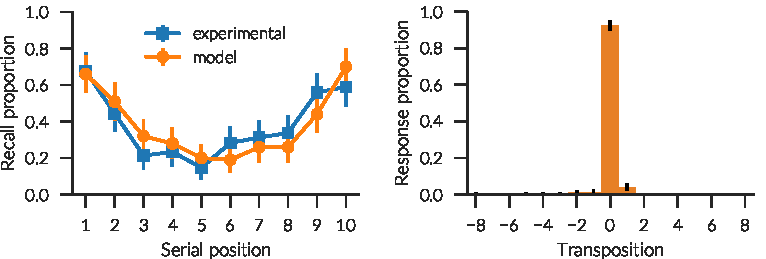
\includegraphics{figures/results/serial}
    \caption[Serial position curve and transpositions for serial recall with the CUE model.]{Serial position curve (left) and transpositions (right) for the serial recall of a \num{10}~item list with the CUE model. The experimental data from \textcite{Jahnke1968} is shown for comparison in the serial position curve (blue squares). The error bars show \SI{95}{\percent} confidence intervals.}\label{fig:results-serial}
\end{figure}

The model allows selective disabling of the recall from the STM or LTM component.
Doing so, with appropriate adjustment of the recall noise level to account for the reduced evidence input, shows that the primacy effect is mediated by the LTM, while the recency effect depends on the STM (\cref{fig:results-no_xtm}).
The recall performance without the LTM contribution is also much worse.
This might be the case either because the input to the recall network might need further adjustment or because no rehearsal mechanism is modelled, resulting in drift of the OSE integrator.
\begin{figure}
    \centering
    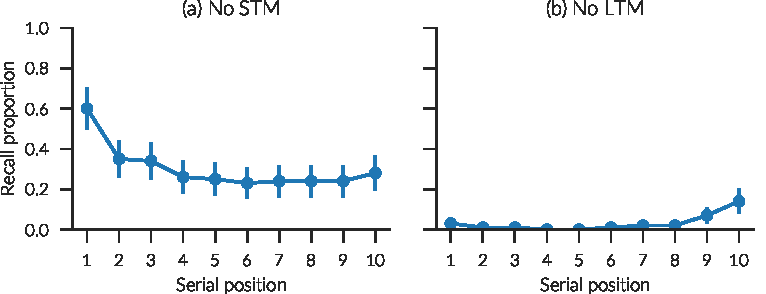
\includegraphics{figures/results/no_xtm}
    \caption[Serial position curves with disabled STM/LTM.]{Serial position curves when either (a) STM recall or (b) LTM recall is disabled in the model.}\label{fig:results-no_xtm}
\end{figure}


\section{Free recall}
While the order of recall is predetermined in serial recall, in free recall list items may be recalled in any order.
Here, I provide the model match to the data from \textcite{Howard1999}, which has also been used in the original fits of the TCM model in \textcite{Howard2002} and \textcite{Sederberg2008}.
Three experimental conditions are matched: immediate recall, delayed recall, and continuous distractor recall.

In the immediate free recall condition, list items are presented at a rate of one item every second.
After the presentation phase, a recall phase of \SI{45}{\second} followed immediately.
This protocol is changed to a presentation rate of one item every \SI{1.2}{\second} and a recall phase of \SI{60}{\second} in the delayed and continuous distractor conditions.
In both of these latter conditions, the presentation and recall phase are separated by a \SI{16}{\second} distractor task.
In addition, in the continuous distractor conditions such a \SI{16}{\second} distractor phase is inserted in between every pair of items.
A list length of 12 items is used in all conditions.
The experimental data was obtained from \num{65}~subjects presented with \num{25}~lists each for the immediate recall condition, and from \num{16}~subjects presented with \num{15}~lists each for the remaining conditions.

Four resulting metrics from the model and experimental data are shown in \cref{fig:results-free}.
First, the distribution of the total number of successful recalls is shown.
To my knowledge, this data has not been analyzed for the original TCM model, even though it is arguably the most fundamental comparison.
In all conditions, the \SI{95}{\percent} confidence intervals of the mean, standard deviation, and kurtosis overlap with the exception of the kurtosis in the immediate recall condition.
Thus, no significant difference for the most essential moments is shown, which indicates that the model approximates the experimental distributions well, even though an equality of the distributions cannot be inferred.
\begin{figure}
    \centering
    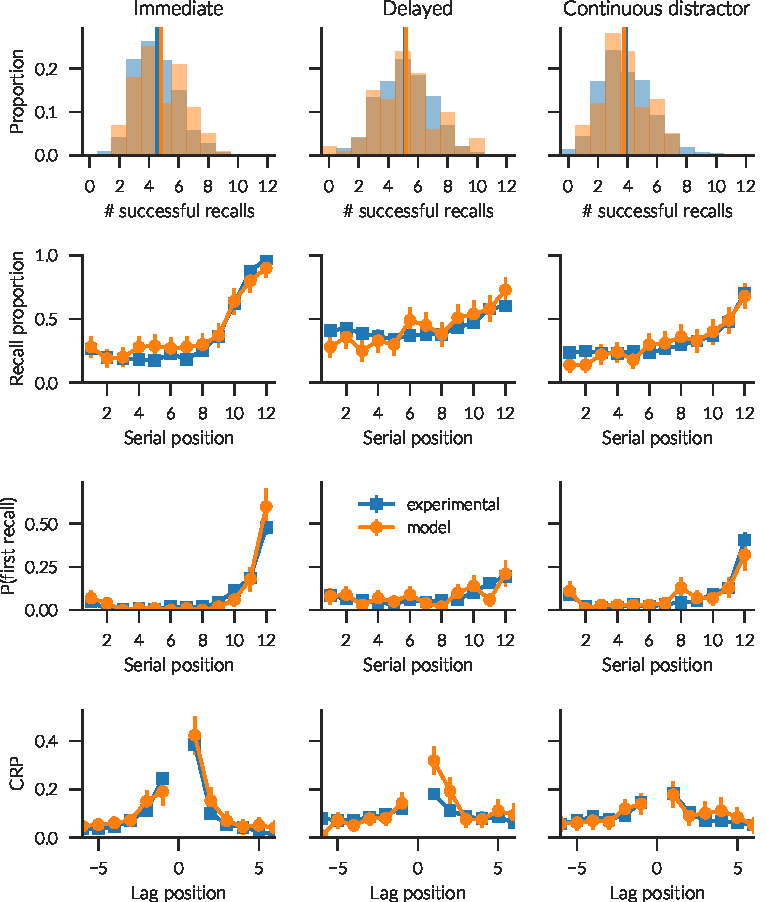
\includegraphics[trim=0 6 0 6]{figures/results/free}
    \caption[Comparison of experimental and model free recall data.]{Comparison of experimental and model free recall data. The columns show the immediate, delayed, and continuous distractor conditions. The rows show from top to bottom: distribution of the number of successful recalls (mean marked by vertical line), serial positions curves, probability of first recall, and the conditional response probability. The error bars show \SI{95}{\percent} confidence intervals. Experimental data by \textcite{Howard1999}.}\label{fig:results-free}
\end{figure}

Second, the serial position curves are given.
The strong recency effect in immediate recall is attenuated in delayed recall, but reappears to some degree in continuous distractor recall.
Interestingly, the recency effect in immediate recall gives the curve an S-like shape that is missing in continuous distractor recall.

Third, these effects also show in the probability of first recall.
In immediate recall, the first recall is, with high probability, from the end of the list, whereas in delayed recall the probability is much more uniform.
In continuous distractor recall, the probability to start the recall at the end of the list is partially restored.

Finally, the conditional response probability (CRP) gives the probability of how much lag there is between the positions of two recalled items is.
For example, the asymmetry in immediate recall shows the bias to do forward recall and the peak around zero that nearby items tend to be recalled together.
Both of these effects become attenuated in delayed and continuous distractor recall.
In delayed free recall, the model predicts a stronger forward bias than the experimental data shows.

The model provides an excellent fit on most measures.
The confidence intervals of \num{101} of the \num{108} data points overlap.
This amounts to less than \SI{7}{\percent} confidence intervals that do not overlap, while about \SI{5}{\percent} are expected to be non-overlapping by pure chance given a \SI{95}{\percent} confidence level.
The most salient deviation of the model and experimental data is observed in the CRP curve for the delayed recall condition.
The model predicts a slightly higher forward bias than is actually found.


\section{Scopolamine}
A spiking neural network model allows the investigation of the effects of drugs more readily than a pure mathematical model.
I demonstrate this here with the acetylcholine antagonist scopolamine.
Administered before the presentation phase in an immediate recall experiment, scopolamine is detrimental to recall performance \parencite{ghoneim1975}.
However, scopolamine administered in between the presentation and recall phase does not influence performance.
This indicates that scopolamine prevents encoding of new memories in LTM, but does not prevent recall of already encoded memories.
More precisely, scopolamine has been shown to attenuate long-term potentiation in hippocampus \parencite{leung2003,ito1988,hirotsu1989-1}.

To model the effect of scopolamine on LTP, A adjusted the AML learning rate for learning the $\mtf$ and $\mft$ matrices.
With this approach the experimental results obtained by \textcite{ghoneim1975} from \num{36}~subjects (\num{8} trials each) are reproduced.
I focus here on the immediate recall experiment with \num{16}~item word lists.
The simulation protocols were again modeled to replicate the experimental settings, with a presentation time of two seconds per item.
To obtain a similar effect, the normal AML learning rate was used before the time point of scopolamine injection and in placebo trials.
After the time point of scopolamine injection it was scaled set to zero.

\Textcite{ghoneim1975} reported a recall accuracy of \SI{77.92(494)}{\percent} (mean $\smash{\pm}$ standard error) in the placebo condition and a recall accuracy of \SI{31.67(228)}{\percent} in the scopolamine condition.
The model produces recall accuracies of \SI{74.18(108)}{\percent} and
\SI{37.94(99)}{\percent}
respectively.
Moreover, the serial position curve for the scopolamine condition shows no primacy effect, but a recency effect (\cref{fig:scopolamine-serial}).
\begin{figure}
    \centering
    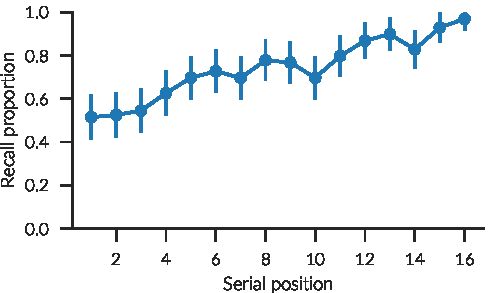
\includegraphics{figures/results/scopolamine-serial}
    \caption{Serial position curve with a scopolamine injection predicted by the CUE model.}\label{fig:scopolamine-serial}
\end{figure} 


\section{Hebb repetition effect}
The simulations for the Hebb repetition effect where modelled after \textcite{Hebb1961}.
A total of \num{25} model instances, equivalent to the \num{25} experimental subjects, were run for \num{24} consecutive trials each.
Each trial consisted out of a nine item list (of the digits from one to nine in random order) and starting with the third trial every third list was identical.

While the model performance seems to slightly worse overall, the qualitive Hebb repetititon effect is reproduced (\cref{fig:hebb}).
\begin{figure}
    \centering
    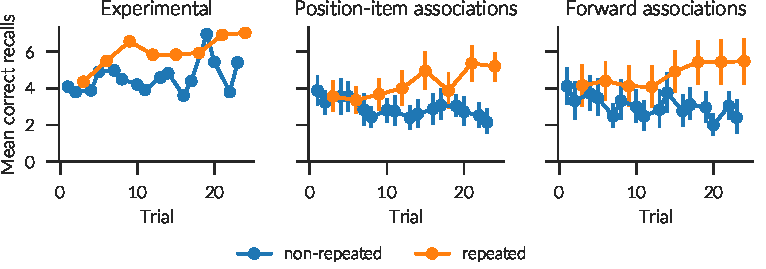
\includegraphics{figures/hebb}
    \caption[Hebb repetition effect.]{Experimental and model data showing the Hebb repetition effect. Nine item lists were presented and one list was repeated on every third trial. From left to right: experimental data \parencite{Hebb1961}, model data with direct learning of position to item associations, and model data with learning of forward associations. The error bars denote \SI{95}{\percent} confidence intervals.}\label{fig:hebb}
\end{figure}
In both, the experimental and all sets of model data, the number of correct recalls increases by about three items on the repeated list.


\section{Memory encoding}
As a spiking neural network model, the CUE model allows the recording of spikes and examination of changes in neural firing (\cref{fig:spikes}).
The distribution of active neurons changes for the STM neurons with each item, with a delay of about \SI{250}{\milli\second} to encode the new item.
When no new item is present, persistent neural firing preserves the firing pattern.
Similar behaviour is observed for neurons encoding the current context signal that gets updated with about a \SI{100}{\milli\second} delay.
The LTM for $\mtf$ (and $\mft$, but not shown) is encoded in neural weights that change for each list item to encode the newly learned associations.
\begin{figure}
    \centering
    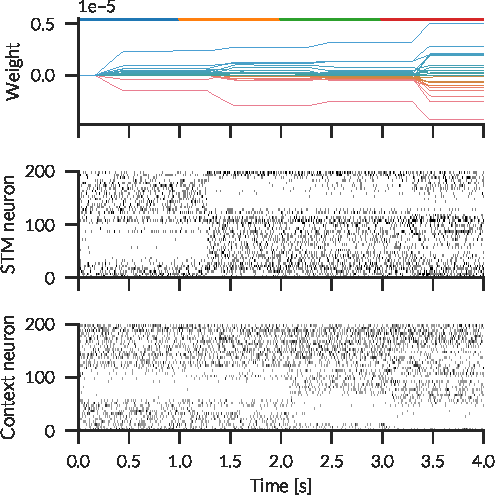
\includegraphics{figures/spikes}
    \caption[Memory encoding in the CUE model.]{Memory encoding in the CUE model. From top to bottom: weights encoding $\mtf$ in LTM, spiking activity of a subset of STM neurons, and spiking activity of a subset of neurons encdoing the context signal $\ctx$. The colored bars at the top mark the presentation of four list different list items.}\label{fig:spikes}
\end{figure}

\chapter{Discussion}
In this thesis, I presented the context-unified encoding (CUE) model.
To my knowledge, it is the first spiking neural network model of human memory that integrates activity-based short-term memory and weight-based long-term memory.
The same model matches a variety of behavioural data from serial and free recall experiments, but in contrast to previous models provides a hypothesis of a neural mechanistic explanation.

The CUE model exhibits many of the hallmark findings in memory research.
It shows the primacy and recency effect in immediate serial and free recall.
These effects get attenuated in delayed free recall, but in continuous distractor free recall the recency effect reappears.
Furthermore, the model was found to make very few transposition errors in serial recall, and if it does so nearby items are transposed.
In the free recall conditions, the model tends to start with items at the end of the list, recall nearby items together, and favour recall in forward direction.
Introducing delays and distractors attenuates these effects.
All of these observations match the findings from experiments with human subjects.

Not only are these qualitative effects reproduced, but also the quantitative match to the data is very good.
Only few significant differences, close to the number of differences expected by chance, were found.
One of these differences is worth considering in more detail: the model predicts a too strong forward bias in delayed free recall with both the lag \num{1} and \num{2} values of the CRP curve being significantly above the experimentally found values.
Interestingly, this is also highlighted as the least well matched aspect in the original TCM \parencite{Howard2002}.
While in that publication the TCM prediction is closer to the experimental data, the TCM prediction from a more recent paper \parencite{Sederberg2008} is closer to the CUE model prediction.
This makes it likely that the difference is not based on pure statistical chance, but that both the TCM and CUE model do not capture an essential aspect of memory, potentially related to the evolution of the context signal, that leads to reduced forward bias in delayed free recall.
It remains for future work, to precisely identify the reason for this mismatch and to extend the model.

Extending CUE model with slow learning of either direct position to item associations or forward associations, allowed to reproduce the Hebb repetition effect qualitatively.
The involvement of such secondary learning should be considered a model prediction, as the effect could not be obtained without this extension.
Modelling the Hebb repetition effect also extends the model to effects across multiple trials of memory experiments.
This is done by only few memory models, in particular, neither the OSE, nor the TCM model attempted to match this such data.

As opposed to pure math models, the implementation as a spiking neural network allows the comparison and validation of the model against data from neural recordings in addition to the behavioural data.
In \cref{sec:aml-neural}, it was demonstrated that the proposed mechanism of association learning is able to explain neural data.
Unfortunately, neural data recorded from humans in memory experiments is still scarce, because invasive recordings can only be done when such recordings are required for medical reasons.
Nevertheless, implementing models with spiking neurons is worthwhile for several other reasons, despite the more complicated model construction and increased simulations times.
Drug effects, like scopolamine, can be more readily modelled, as was done with CUE model.
Also a higher degree of biological plausibility is achieved as one is forced to consider, for example, spiking noise and synaptic time constants.
This prevents common assumptions like arbitrary precision or perfectly orthogonal vectors made in many math models.

The spiking neural implementation also helps to constrain many parameter values.
Synaptic time constants, membrane time constants, and similar cellular physical quantities can be set to biologically plausible values reported in experimental findings.
These are fixed parameters that have not been adjusted for matching the behavioural data.
Similarly, as in the NEF, most connection weights are directly determined by least-squares minimization to implement a given function determined by the prescribed model architecture, hence the connection weights are fixed as well.
This leaves the model with very few free parameters.

To match the immediate serial recall, only two parameters were adjusted: the bias of the null choice $\minev$ and the input noise standard deviation $\recnoise$ in recall.
Both account for the fact that the recall network was restricted to recalling the items used within the memory experiment, while in reality a number of other items might interfere with the recall process.
For free recall experiments, one additional parameter $\psi$ is added that determines the probability of using the serial recall strategy even for free recall.
(For serial recall, a fixed values of $\psi = 1$ is implied as no free recall is allowed.)
Furthermore, in experiments with delay periods, a distractor rate $\drate$ needs to be set.
To simulate the effect of scopolamine the AML learning rate $\eta$ was adjusted.
However, in non-scopolamine conditions, it was treated as a fixed parameter and set to a value high enough to learn associations until the threshold for inhibition was achieved within the presentation duration.
Even higher values would not have any effect as long as it does not largely exceed the inverse of the synaptic time delay of the inhibition.
Lastly, only two additional parameters (weight decay rate and a separate learning rate) were introduced by the model extension to the Hebb repetition effect.

While few free parameters are desirable with respect to model parsimony, they should also be assigned similar values to model-related experimental conditions.
This is mostly the case for the CUE model.
The bias of the null choice in recall ranges from \numrange{0.03}{0.04} and values get monotonously smaller as the task difficulty increases with additional delays.
This corresponds to plausible longer recall attempts in more difficult experimental conditions.
Only a small difference is also observed in the distractor rates (\numrange{0.3}{0.4}) and the probability of using a serial recall strategy (zero for delayed recall and \num{0.1} in all other free recall conditions).
However, the noise standard deviation $\recnoise$ in recall differs by a factor of more than \num{1.5} without a clear relation to the experimental condition.
It is hard to hypothesize potential reasons for this difference as the parameter is accounting for things not explicitly modeled in recall.

It is also of interest how robust the model is against parameter changes.
I have not done a formal analysis of this because the model simulation times are prohibitive.
However, this also means that only a small set of parameter values without a lot of fine tuning has been tested (less than \num{200} combinations summed over all experimental conditions).
Given that finding the right parameters with few simulations is less likely if the model were highly sensitive to the parameter choice, a sufficient robustness to the exact choice of parameter values can be expected.

The CUE model is based on prior models of memory, but improves on them in important ways.
With regard to the OSE model, two main advancements can be stated.
First, the episodic memory buffer has been replaced with a much more plausible long-term memory mechanism that relies on synaptic-weight changes rather than reverberating neural activity.
Second, the CUE model also implements the mechanism providing the position tags fully in spiking neurons.

Implementing a long-term memory component based on the TCM in a spiking neural network provides a strong support for the biological plausibility of the TCM that previously was missing.
Certain simplifications of the TCM equations in this process to facilitate this implementation highlight which aspects of the TCM are essential and which do not contribute to the explanation of the data.
In particular, it also shows that certain assumptions, like perfectly orthogonal vectors, useful in the mathematical analysis, are not essential.
In addition, the modified TCM has been extended with a short-term memory component in the CUE model.
While the TCM has been posited as a single-store model, this has been criticized \parencite{Davelaar2008}.
The CUE model demonstrates that treating the TCM as part of a multi-store model is not unreasonable, provides good matches to the free recall data, and in addition allows matches to serial recall data.
Finally, the recall process in the TCM was not modeled in a particularly biologically plausible way and has been replaced with a more plausible spiking neural mechanism (\cref{sec:recall}).

In the broader context of memory models, the CUE model is unique as providing a low-level spiking network implementation, but matching high-level behavioural data.
This includes the recall process that is not explicitly modeled in many other models.
Furthermore, due to the item based context, there is no reinstantiation problem found in most context-based memory models.

A key part of the CUE model is the association matrix learning rule.
It provides insight into how one-shot learning without catastrophic forgetting is possible.
Several options and their biological plausibility of how this learning rule might be realized in the brain have been discussed in \cref{sec:aml}.
The main point there is that either some form of weight-sharing or symmetric decoder matrix is needed, or the input needs to be transformed into a sparse representation.
The dentate gyrus of the hippocampus exhibits such sparse firing and is implicated in associative learning, giving support to the latter hypothesis.
However, I also provided evidence that a symmetric decoder matrix might be learned in a biological plausible way.
Moreover, using the AML for learning simple pairwise associations, allows the reproduction of changes in firing rates that have been observed in recordings from human hippocampus.
These results are not only of interest for the CUE and TCM models, but many other cognitive models that assume the storage of associations in a similar association matrix without further explanation of how these associations are learned.

One potential criticism of the CUE model could target the way of position counting (\cref{sec:posnet}).
Only a limited number of positions can be represented, even though this number can be configured as large as permitted by neural resources.
If the number of positions is exceeded, the representation can be made to wrap around back to the first position.
Thus, the model does not need to fail catastrophically, but a specific pattern of recall errors could be introduced by encoding different sequences of items to the same positions.
However, an experimental test of such predictions will be hard, as long lists are likely required, and thus for most position no item at is recalled.
It is worth to highlight that the position counting network in the CUE model can be replaced easily to test other hypotheses.
But it seems unlikely that the limited number of positions can be eliminated completely, because there will always be a limited number of almost orthogonal Semantic Pointers that fit into a vector space of given dimensionality.


%\begin{itemize}
    %\item firing rates!
    %\item basal ganglia involvement?
    %\item Control is the hard part
    %\item exact implementation of experimental protocol
    %\item fuzzy temp memory sensitive to noise and thus no alternative for context signal
%\end{itemize}


\section{Anatomical mapping}

Given that the CUE model is neural, it is of interest to consider how the parts of the model map to brain areas.
\Textcite{howard2005} proposed a mapping of the TCM model to brain areas that applies to a large degree also to the TCM-based part of the CUE model.
There are, however, some details to be reconsidered, and the OSE-based STM part of the model has not been discussed.

The medial temporal lobe (MTL) is known to be essential for free recall.
Damage to the MTL is detrimental to free recall performance \parencite{graf1984}.
Thus, we can assume that the TCM-related parts of the model reside in the MTL\@.

More precisely, the context storage network can be mapped  onto parahippocampal areas, in particular the entorhinal cortex (EC).
Its properties are consistent with the storage of non-spatial memories for tens of seconds.
In delay periods, stimulus dependent persistent activity can be observed \parencite{suzuki1997,young1997}.
\Textcite{quirk1992} showed EC has a higher mean firing rate than hippocampus, which is not caused by short bursts, and is thus compatible with the sustained maintenance of neural firing.
Also, the electrophysiological properties of the EC support integration \parencite{egorov2002}.
These findings are, however, based on intrinsic cell properties, whereas the CUE model uses recurrent connectivity for integration instead.
Note that the context network also contains integration ensembles that maintain the context signal over the timespan of seconds.

While the EC firing is modulated to some degree by the item position, this coding is more noisy than in the hippocampus \parencite{quirk1992}.
This indicates that EC codes for additional information.
\Textcite{Frank2000} have shown that superficial EC employs retrospective coding, i.e., that it differentiates visits to the same position by the history leading up to that visit.
This is consistent with a context signal encoding the history of items leading up to the current item.

The other major components to map to brain structures are related to the learning and retrieval of associations in the $\mft$ and $\mtf$ matrices.
\Textcite{howard2005} stated that the $\mft$ matrix might not be implemented by a single anatomical region due to its complicated structure.
However, the updating equation for $\mft$ in the CUE model has been simplified, which makes the correspondence to a single region more plausible.
The learning of new associations in these matrices is attributed to the hippocampus by \textcite{howard2005}.
This is consistent with the results about the AML presented in \cref{sec:aml}.

The CUE model provides a more detailed description of the updating of the association matrices due to the neural implementation by means of the AML\@.
The learning network has recurrent connectivity to inhibit the learning once an association has been learned with the desired strength.
Recurrent connectivity is also found in the CA3 region of hippocampus.
Furthermore, CA3 receives input via the dentate gyrus and directly from entorhinal cortex, which could correspond to separate transmission pathways for the associated cue and target.
Interestingly, the AML highlighted the need to incorporate the decoder matrix $\mdec\Tr$ into the connections.
While I have shown it might be plausible that this connectivity is learned, the matrix could be reduced to the identity if the input ensemble were to provide orthogonalized inputs.
The dentate gyrus, providing input to CA3, is commonly assumed to perform such orthogonalization given its large neuron count, sparse firing, and neurogenesis \parencite[e.g.,][]{boss1987,jung1993-1,piatti2013}.
Thus, while the CUE model does not explicitly model the dentate gyrus (which is a significant research problem in itself), the learning rule used at least provides a principled reason for its existence.

Further evidence for this neuroanatomical mapping can be obtained from the connectivity between hippocampus and EC\@.
The superficial EC provides input to hippocampus, but does not receive direct input for hippocampus \parencite{witter2010}.
In contrast to that, the deep layers of EC receive input from hippocampus and might be relevant for recall, especially the recall of pre-experimental context.
This is consistent with the connectivity in the model where the context network projects to the association matrix learning network attributed to hippocampus.
The learning network for $\mft$ also projects back to an ensemble recalling the prior context before it gets combined in a different ensemble.

The short-term memory related components of the CUE model can be assumed to correspond to cortical areas, in particular the prefrontal cortex.
The prefrontal cortex has been found to be involved in working memory tasks in many studies \parencite[e.g.,][]{goldman-rakic1995,owen1997}


\section{Optimally fuzzy temporal memory}\label{sec:fuzzymem}
\Textcite{shankar2013} proposed a mathematical model of an optimally fuzzy temporal memory.
According to them it can replace the context signal in the TCM \parencite{howard2015}.
Thus it could also be relevant to the CUE model, but I argue below that a spiking neural version of this memory is unlikely to work without an implausible number of neurons.

The fuzzy temporal memory is constructed with the aim of representing past values of a function $f(t)$ with a scale-free fall off in accuracy.
Note that multiple such fuzzy temporal memories could be combined to represent a vector-valued function as needed for the context signal in the TCM or CUE models.
The memory itself consists of a set of independent, leaky accumulators given by the differential equation
\begin{equation}
    \od{c_i(t)}{t} = - s_i c_i(t) + f(t)
\end{equation}
where $s_i$ are decay constants.
This set of integrators is essentially computing a Laplace transform.
To readout the memory, the Laplace transform is inverted approximately with a linear operator $\mat L_k^{-1}$ given by
\begin{equation}
    \sbr{\mat L_k^{-1}}_{ij} = \frac{{(-1)}^k}{k!} s_i^{k+1} \sbr{\mat D_k}_{ij}
\end{equation}
where $\mat D_k$ is a square matrix that computes the $k$-th discrete derivative with respect to $s$.
The reconstructed $\hat{f}_t(t + t^*) = \sbr{\mat L_k^{-1} \vc c(t)}_i$ with $t^* = -k/s_i < 0$ estimates the values of $f$ at times $t + t_i^*$ in the past.
The reconstruction becomes more accurate as $k \rightarrow \infty$.

\Textcite{shankar2013} derive a signal to noise ratio, but use the magnitude of a delta impulse input to do so.
As the magnitude of a delta impulse is infinite in the limit, the signal to noise ratio also grows without bound for $k \rightarrow \infty$.
However, it is physically impossible to deliver a perfect delta impulse.
Instead it is more appropriate to analyze the steady state response for a fixed input $f(t) = u$.
In the context of the NEF, $u=1$ can be assumed without loss of generality because any change in the magnitude $u$ requires a matched change in the representational radius $\radius$ which will also scale the absolute error, keeping the relative error the same.
The steady state of the leaky integrators is then given by $c_i(t) = s_i^{-1}$.
This implies that NEF ensembles representing $c_i$ should use a radius of $\radius = s_i^{-1}$.

The amplification of the noise standard deviation is given by \textcite{shankar2013} as
\begin{equation}
    g_{\eta}(s_i, k) = \frac{\sqrt{2^k} s_i^{k+1}}{\delta_{s_i}^k k!}
\end{equation}
where $\delta_{s_i} = s_i - s_{i - 1}$. 
When following their proposal for optimal spacing of the $s_i$ by picking $t_i^* = (1 + \nu)^{i - 1} t_1^*$ for some constant $\nu > 0$, it follows that $\delta_{s_i} / s_i = \nu$ and the formula can be simplified to
\begin{equation}
    g_{\eta}(s_i, k) = \frac{\sqrt{2^k} s_i}{\nu^k k!} = - \frac{\sqrt{2^k}}{\nu^k (k-1)! t_i^*} \text{.}
\end{equation}
Note that this amplification is not independent of $t_i^* = -k/s_i$, but increases as $t^* \rightarrow 0$.
This can be seen easily when adding some Gaussian noise to all $c_i$ before the reconstruction as done in \cref{fig:fuzzy-mem-noise-example}a.
It also refutes that ``the signal to noise ratio will remain constant over all timescales'' \parencite{shankar2013}; a statement based on the assumption of a perfect delta impulse.
However, as stated above, NEF ensembles should use a radius of $\radius = s_i^{-1}$ which scales the noise by the same factor and thus indeed leads to a constant amplification of the noise across timescales (\cref{fig:fuzzy-mem-noise-example}b) given by
\begin{equation}
    g_{\eta,\ped{NEF}}(\nu, k) = \frac{\sqrt{2^k}}{\nu^k k!} \text{.}
\end{equation}
\Cref{fig:fuzzy-mem-noise-ts}a shows this amplification for different parameter values.
When both $\nu$ and $k$ are chosen large enough, noise will actually be attenuated.
However, this also increases the timescale (\cref{fig:fuzzy-mem-noise-ts}b) and as such there is a trade-off between the time resolution of the memory and noise amplification.
This increase in timescale is given by
\begin{equation}
    \tau_i(\nu) = - {(1 + \nu)}^k t^*_i \label{eqn:fuzzymem-ts}
\end{equation}
and is caused by the discrete approximation of the derivative that relies on $t^*_{i - k}$ to $t^*_{i + k}$ for the reconstruction of $\hat{f}_t(t + t^*_i)$ and is dominated by $t^*_{i + k}$ (\cref{apdx:fuzzymem-derivative}).
\begin{figure}
    \centering
    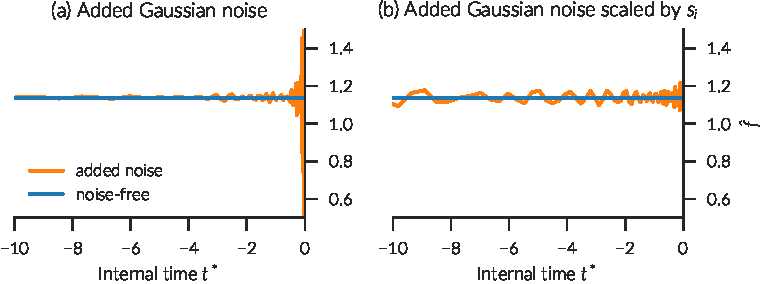
\includegraphics{figures/fuzzy-mem-noise-example}
    \caption[Example of the effect of noise on the fuzzy temporal memory.]{Examples of the effect of noise in the leaky integrators $c_i$ of the fuzzy temporal memory on the reconstruction $\hat{f}$. (a) Gaussian noise with mean zero and a constant standard deviation is added to the output of all integrators. (b) Gaussian noise with mean zero and standard deviation scaled by $s_i^{-1}$ is added to the output of all integrators.}\label{fig:fuzzy-mem-noise-example}
\end{figure}
\begin{figure}
    \centering
    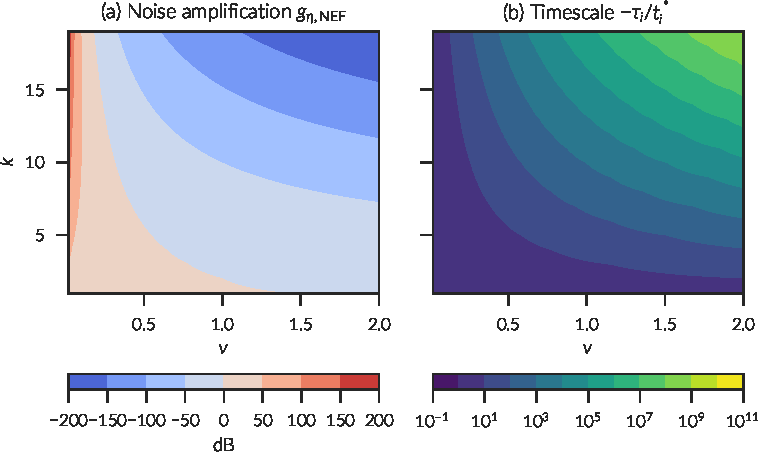
\includegraphics{figures/fuzzy-mem-noise-ts}
    \caption[Noise amplification and timescales in fuzzy temporal memory.]{(a) Noise amplification $g_{\eta,\ped{NEF}}$ in the fuzzy temporal memory. (b) Timescale $\tau_1$ for the $t^*_1$ reconstruction of the fuzzy temporal memory.}\label{fig:fuzzy-mem-noise-ts}
\end{figure}

Based on these equations, the total number of neurons $N_{\ped{tot}}$ required can be estimated as (\cref{apdx:fuzzymem-neurons})
\begin{align}
    N_{\ped{tot}}(t^*_1, k) &= N \dims\, g_{\eta,\ped{NEF}}^2(\nu, k) \del{M + 2k} \label{eqn:fuzzy-n-neurons}\\
    M &\geq \frac{\log(t^*_{\max} / t^*_1)}{\log(1 + \nu)} \\
    \nu &\leq \sqrt[k]{-\tau_1 / t^*_1} - 1
\end{align}
where $N$ is the number of neurons to represent a single dimension with sufficient accuracy (before the effect of the noise amplification), $\dims$ is the dimensionality of the input signal, $M$ gives the number of required leaky integrators, $\tau_1$ gives the desired smallest timescale, and $t^*_{\max}$ gives the desired timespan of the fuzzy memory.
Assuming that the fuzzy temporal memory is to be used for the TCM context signal, $\tau_1 \leq \SI{1}{\second}$ and $t^*_{\max} \geq \SI{10}{\second}$ are reasonable choices because ten item lists with a presentation rate one item per second are typical for the memory experiments matched in this work.
Furthermore, $N = 50$ and $\dims = 64$ can be used as conservative estimates.
Using \num{50}~neurons with maximum firing rates between \SIrange{200}{400}{\second^{-1}} is sufficient to read out the represented value, but not very precisely.
This default range of firing rates is much higher than firing rates typically observed in vivo.
Thus, the actual required number of neurons can be expected to be higher.
A dimensionality of $\dims = 64$ is also on the lower end to be able to fit sufficiently many almost orthogonal vectors into the space.
The CUE model uses four times as much, $\dims = 256$, dimensions.
Ultimately, the choice of $N$ and $\dims$ has only a minor influence on the results as they are just linear factors while the required number of neurons grows exponentially for $t^*_1,\ k \rightarrow \infty$.
The results for this choice of parameter values is shown in \cref{fig:fuzzy-mem-n-neurons}.
For most parameter combinations, the number of about $\num{13e6}$ neurons in the entorhinal cortex \parencite{west1998}, assumed to be the locus of the CUE/TCM context signal, and even the number of about \num{86e9} neurons in the human brain \parencite{azevedo2009} is far exceeded.
For an implementation with a realistic limit on the neuron number, $t^*_1$, but also $k$, needs to be sufficiently small.
\begin{figure}
    \centering
    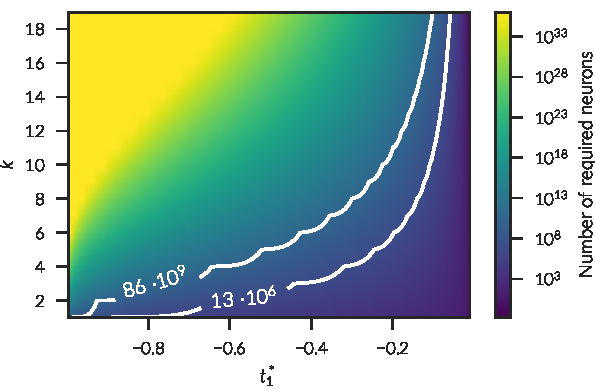
\includegraphics{figures/fuzzy-mem-n-neurons}
    \caption[Number of neurons required to implement a fuzzy temporal memory.]{Number of neurons required to implement a fuzzy temporal memory with a lower timescale of $\tau_1 = \SI{1}{\second}$ and a timespan of $t^*_{\max} = \SI{10}{\second}$. The white contours give the approximate number of neurons in the human entorhinal cortex (\num{13e6}) and human brain (\num{86e9}). See text for further details.}\label{fig:fuzzy-mem-n-neurons}
\end{figure}

Unfortunately, choosing small $t^*_1$ and $k$ is also problematic.
The error of the approximate inversion of the Laplace transform with Post's formula converges only at a rate of $1/k$ \parencite{vukimtuan2000}.
\Textcite{shankar2013} also comment themselves that $t^*_1$ needs to be kept sufficiently far from zero as it introduces a relative error in the order of $\bO\big(k^3\nu^2/96 t^{*2}_1\big)$ in the construction of the activity of $c_i$.

In conclusion, the fuzzy temporal memory has only a small parameter space that allows an implementation with feasible neural resources due to noise sensitivity.
This parameters space suffers from large relative errors unrelated to noise in the approximation of the inverse Laplace transform and discretized derivative.
Currently, it is not clear whether these non-noise related errors are sufficiently small to allow the fuzzy temporal memory to be used as a context signal in the CUE model.
At the same time it would require an increased number of neurons compared to the current implementation as each dimensions requires a set of leaky integrators, i.e.\ additional values have to be stored for each dimensions.
In comparison, the context network for \num{256}~dimensional vectors uses only \num{51225} neurons, and even when adjusting by a factor of \num{10}, this is many fewer neurons than found in the entorhinal cortex.


\section{Advances in large-scale cognitive modeling}
The primary objectives of building the CUE model lead to a number of advances in large-scale cognitive modeling that are worth summarizing, even though not all have been presented as part of this thesis.
Most importantly, optimizations for high-dimensional representations in neural networks (\cref{sec:hdrep};\ \cite{gosmann216}).
These allow the use of fewer neurons in such models, which ultimately allows more complex networks to be built without prohibitively long simulation times.
A similar benefit is the improved product network \parencite{gosmann2015-1}, as the calculation of products is often required, for example for the implementation of circular convolution.
Also a significant improvement to simulation times was achieved by the implementation of an optimization procedure in the Nengo simulator \parencite{gosmann2017}.
\Cref{sec:spa} described a new method for binding Semantic Pointers, the vector-derived transformation binding.
Even though it has not been used in the CUE model yet, it might provide a more precise binding and unbinding.
Finally, the independent accumulator network described in \cref{sec:ia} might not only be useful in recall, but for other large-scale models requiring clear decisions as part of a cognitive process.

\section{Anatomical mapping}

Given that the CUE model is neural, it is of interest to consider how parts of the model map to brain areas.
\Textcite{howard2005} proposed a mapping of the TCM model to brain areas that applies to a large degree also to the TCM-based part of the CUE model.
There are however some details to be reconsidered and the OSE-based short-term part has obviously not been discussed.

The medial temporal lobe (MTL) is known to be essential for free recall.
Damage to the MTL is detrimental to free recall performance \parencite{graf1984}.
Thus, we can assume the TCM related parts of the model to reside in the MTL (TODO figure).

More precisely, the context storage network can be mapped  onto parahippocampal areas, in particular the entorhinal cortex (EC).
Its properties are consistent with the storage of non-spatial memories for tens of seconds.
In delay periods stimulus dependent persistent activity can be observed \parencite{suzuki1997-1,young1997}.
\Textcite{quirk1992} showed EC has a higher mean firing rate than hippocampus which is not caused by short bursts and is thus compatible with the sustained maintenance of neural firing.
Also, the electrophysiological properties of the EC support integration \parencite{egorov2002}.
These findings are, however, based on the intrinsic cell properties, whereas the CUE model uses recurrent connectivity for integration instead.
Note, that the context network does contain integration ensembles that maintain the context signal over the timespan of seconds.

While the EC firing is modulated to some degree by the position, this coding is more noisy than in the hippocampus \parencite{quirk1992}.
This indicates that EC codes for additional information.
\Textcite{Frank2000} have shown that superficial EC employs retrospective coding, that it differentiates visits of the same position by the history leading up to that visit.
This is consistent with a context signal encoding the history of items leading up to the current item.

The other major component to map to brain structures are the learning and retrieval of associations in the $\mft$ and $\mtf$ matrices.
\Textcite{howard2005} stated that the $\mft$ matrix might not be implemented by a single anatomical region due to its complicated structure.
However, the updating equation for $\mft$ in the CUE model has been simplified which makes the correspondence to a single region more plausible.
The learning of new associations in these matrices is attributed to the hippocampus by \textcite{howard2005}.
TODO more details.
Though, they do not consider the retrieval to be dependent on the hippocampus because TODO\@.

TODO because of striatal association learning?
Simple associations of same modality might be learned there, but cross-modality and integration (i.e.\ of item and context) might happen in hippocampus.
But striatum seems to be mostly for reward associations like in Pavlovian conditioning and other reward/punishment learning.

The CUE model provides a more detailed description of the updating of the association matrices due to the neural implementation by means of the AML\@.
In the learning network we get recurrent connectivity between TODO\@.
This is analogous to recurrent connectivity in the CA3 region of hippocampus.
TODO additional input via different pathways.
Moreover, the AML highlighted the need to incorporate the decoder matrix $\mdec\Tr$ into the connections.
While I have shown it might be plausible that this connectivity is learned, the matrix could be reduced to the identity if the input ensemble were to provide orthogonalized inputs.
The dentate gyrus, providing input to CA3 is commonly assumed to perform such orthogonalization given its large neuron count, sparse firing, and neurogenesis (TODO refs).
Thus, while the CUE model does not explicitly model the dentate gyrus (which is a significant research problem in itself), the learning rule used at least provides a principled reason for its existence.

Further evidence for this neuroanatomical mapping can be obtained from the connectivity between hippocampus and EC\@.
The superficial EC provides input to hippocampus, but does not receive direct input for hippocampus (TODO ref).
In contrast to that, the deep layers of EC receive input from hippocampus and might be relevant for recall, especially the recall of pre-experimental contex.
This is consistent with the connectivity in the model where the context network projects to the association matrix learning network attributed to hippocampus.
The learning network for $\mft$ also projects back to an ensemble recalling the prior context before it gets combined in a different ensemble.


TODO did they actually say anything about context-to-item matrix?

more going on in MTL, eg place cells

\chapter{Conclusion}
To summarize, the context-unified encoding model advances our understanding of human memory by matching human behavioural data using an implementation grounded in a spiking neural network.
The difficult task of building a spiking neuron model of this scale also led to a number advances in large-scale cognitive modeling in general, such as high-dimensional neural representations with reduced noise.
Despite this, the CUE model is only a first step in the integration of neural and behavioural data as well as the understanding the interaction of short- and long-term memory.
Much more data from memory experiments exists that could be matched, and can be used to highlight where the CUE model is wrong or needs to be extended.
One such aspect that was already evident is the strength of the forward recall bias in delayed free recall.
Future work could also focus on mapping the long-term memory components more precisely onto hippocampal structures and cellular properties in the relevant regions.
In particular, introducing sparsification with a dentate gyrus model could improve the biological plausibility of the AML\@.

The sequences that the CUE model can memorize are much simpler than the fidelity of actual human memory.
But they have been proven useful in psychology to investigate basic properties of memory.
Also, many forms of memory can be understood as a sequence:
episodic memory is essentially a sequence of events or a sequence of left and right turns might be necessary to navigate from one place to another.

Finally, the CUE model, in the broader context of large scale cognitive modeling, could provide an excellent extension to the Spaun model.
A proper long-term memory component is missing from this model so far, despite being essential for cognition.
The CUE model itself could also benefit from such an integration, as Spaun's ability to perform multiple tasks would allow to model experimental delay phases with an actual distractor task.


\addchap{Acknowledgements}
IK
Sharcnet/compute canada + their support team
Nengo development team and opportunities

\printbibliography[heading=bibintoc,title=References]

\appendix
\addpart{Appendices}
\chapter{Derivation of the cosine similarity distribution}\label{apdx:cosine-sim}
\begin{proof}
A straight-forward way to derive the cosine similarity distribution is to use a result by \textcite{cai2013}.
Theorem~1 states that the probability density of the angles $\theta$ between independent $\dims$-dimensional vectors is given by
\begin{equation}
    h(\theta) = K_{\dims} \cdot \del{\sin \theta}^{\dims - 2},\quad \theta \in \sbr{0, \uppi}
\end{equation}
with
\begin{equation}
    K_{\dims} = \frac{1}{\sqrt{\uppi}} \frac{\Gamma\!\del{\frac{\dims}{2}}}{\Gamma\!\del{\frac{\dims - 1}{2}}} = \frac{\Gamma\!\del{\frac{\dims}{2}}}{\Gamma\!\del{\frac{1}{2}} \Gamma\!\del{\frac{\dims - 1}{2}}} = \frac{1}{B\!\del{\frac{1}{2}, \frac{\dims -1}{2}}} \text{.}
\end{equation}
To obtain the cosine similarity distribution a change of variables with $\theta = \arccos x,\ x \in [-1, 1]$ has to be performed:
\begin{align}
    \pcs(x; \dims) &= \abs{\od{}{x} \del{\arccos x}} \cdot h(\arccos x) \\
    &= \frac{1}{\sqrt{1 - x^2}} \cdot K_{\dims} \cdot \del{\sin \arccos x}^{\dims - 2} \\
    &= \frac{1}{\sqrt{1 - x^2}} \cdot K_{\dims} \cdot \del{\sqrt{1 - x^2}}^{\dims - 2} \\
    &= K_{\dims} \cdot \del{1 - x^2}^{\del{\dims - 3}/2} \text{.}
\end{align}
This matches \cref{eqn:pcs}.
\end{proof}

The cosine similarity distribution can also be obtained as a special case of a more general distribution of the $\ell^2$-norm of $m$ components of an $n+m$-dimensional unit vector.
The PDF of this distribution is given by \textcite{harman2010,gosmann216}
\begin{equation}
    p_{\mathcal{SB}}(x; n, m) = \frac{2}{B\!\del{\frac{n}{2}, \frac{m}{2}}} \del{x^2}^{(m-1)/2} \del{1 - x^2}^{n/2 - 1},\quad x \in [-1, 1] \text{.}\label{eqn:psb}
\end{equation}
When determining the cosine similarity of two uniformly distributed random vectors $\vc a$ and $\vc b$, we are free to chose any set of basis vectors without loss of generality.
Let us chose the basis such that $\vc a = (a_1, 0, 0, \dots)\!\Tr$ is aligned with the first vector of the standard basis.
The cosine similarity then becomes
\begin{equation}
    \cos(\vc a \angle \vc b) = \frac{\langle \vc a, \vc b \rangle}{\big\|\vc a\big\| \cdot \big\|\vc b\big\|} = \frac{a_1 \cdot b_1}{a_1 \cdot \big\|\vc b\big\|} = \frac{b_1}{\big\|\vc b\big\|} \text{.}
\end{equation}
The absolute value of this is equal to the length of a one-component subvector of the unit-vector $\vc b/\norm{\vc b}$.
Thus, we can use \cref{eqn:psb} and divide it by two to account for the symmetry of the absolute value to determine the PDF of the cosine similarity as
\begin{equation}
    \pcs(x; \dims) = \frac{1}{2} p_{\mathcal{SB}}(x; \dims - 1, 1) = \frac{1}{B\!\del{\frac{1}{2}, \frac{\dims - 1}{2}}} \del{1 - x^2}^{\del{\dims - 3}/2}\text{.}
\end{equation}

\chapter{Comparisons of the uniform and cosine similarity intercept distributions}\label{apdx:hdrep}
\Cref{tbl:csdist} summarizes the change in error over a wide range of parameters when switching from a uniform intercept distribution to the $\csdist(\dims + 2)$ distribution.
In general, the cosine similarity distribution performs better.
It performs equal to the uniform distribution for $\dims = 1$ in which case $\csdist(\dims + 2)$ reduces to a uniform distribution and rectified linear (rate) neurons with a regularization of $\reg = 0.1$.
The cosine similarity distribution performs slightly worse for rate neurons (LIF rate and rectified linear) when the regularization is adjusted to $\reg = 0.01$ to account for the non-existent spiking noise.
The only other case with slightly worse performance is when computing pairwise products $y_i = x_{2i - 2} x_{2i - 1},\ 1 \leq i \leq i/2$, but note that no further optimization for this sort of function has been done and the high dimensionality makes this a hard function to compute.
On the simpler squaring, the cosine similarity distribution performs better.
\begin{table}
    \begin{addmargin*}[0mm]{-31pt}
        \caption[Comparison of uniformly and $\csdist(\dims + 2)$ distributed intercepts.]{Change in representational error in the NEF when switching from uniformly distributed intercepts to $\csdist(\dims + 2)$ distributed intercepts for different dimensionalities $\dims$, neuron numbers $n$, synaptic time constants $\syntau$, decoded functions, regularization $\reg$, and neuron types.
    A negative change in error (highlighted red) means that the cosine similarity distribution performed better.
    Statistical significance, determined with bootstrapping, is marked with **** for $p < 0.0001$ and * for $p < 0.05$.}\label{tbl:csdist}
        \scriptsize\centering
        \sisetup{
            table-figures-integer=1,
            table-figures-decimal=4,
            table-sign-mantissa,
            table-number-alignment=left,
        }
        \begin{tabular}{S[table-number-alignment=right,table-figures-integer=2,table-figures-decimal=0]S[table-number-alignment=right,table-figures-integer=4,table-figures-decimal=0]S[table-figures-decimal=3]lS[table-figures-decimal=3]lS[table-space-text-post={****},round-precision=4,round-mode=places,scientific-notation=fixed,fixed-exponent=0,negative-color=BrickRed]S[table-space-text-post={****},round-precision=4,round-mode=places,scientific-notation=fixed,fixed-exponent=0,negative-color=BrickRed]S[table-space-text-post={****},round-precision=4,round-mode=places,scientific-notation=fixed,fixed-exponent=0,negative-color=BrickRed]}
\toprule
   &    &       &         &       &              & \multicolumn{3}{c}{Change in} \\
   &    &       &         &       &              &   $\langle\errdist\rangle$ &   $\langle\errnoise\rangle$ &  $\langle\errtotal\rangle$ \\
$\dims$ & $n / \dims$ & $\syntau / \si{\second}$ & Function & $\lambda$ & Neuron type &                            &                             &                            \\
\midrule
1  & 50 & 0.005 & $\vc x$ & 0.100 & LIF &     1.2849080544736352e-05 &       0.0009289477152641251 &      0.0009813160649235486 \\
2  &    &       &         &       &              &      0.0006935373487160466 &   -0.005011356652797429**** &  -0.004319006519981905**** \\
4  &    &       &         &       &              &      -0.002040085331075192 &   -0.013890338543531083**** &  -0.013721351649611621**** \\
8  &    &       &         &       &              &      0.0036561681879286392 &    -0.03181686125505534**** &  -0.026775116022725975**** \\
64 & 10 &       &         &       &              &   -0.12385726519109116**** &    -0.21313656378019652**** &   -0.24577344411013363**** \\
   & 25 &       &         &       &              &   -0.04380034323030774**** &    -0.17432274728926517**** &    -0.1778286359045759**** \\
   & 50 &       &         & 0.005 &              &   0.034684333550832655**** &      -0.283590365358218**** &   -0.27902555939727636**** \\
   &    &       &         & 0.010 & Adaptive LIF &     0.0821060272370703**** &    -0.22492585022544237**** &   -0.17895684535932888**** \\
   &    &       &         &       & LIF &   0.026205643385408477**** &     -0.2190924433586482**** &   -0.21418489823193215**** \\
   &    &       &         &       & LIF Rate &   0.026216644979428466**** &     1.3495558654430138e-15* &   0.026216644979428137**** \\
   &    &       &         &       & Rectified Linear &    0.03065106265473031**** &       5.094502290754735e-16 &    0.03065106265472966**** \\
   &    &       &         & 0.100 & Adaptive LIF &    0.03113217839300403**** &    -0.13152209374136542**** &    -0.0814949509662396**** \\
   &    &       &         &       & LIF &   -0.01998629808658868**** &    -0.13129882048505984**** &   -0.13036370447062218**** \\
   &    &       &         &       & LIF Rate &  -0.019953903694741773**** &       2.354290724182059e-16 &   -0.01995390369474198**** \\
   &    &       &         &       & Rectified Linear &      0.0021980363520863327 &      3.7418367648159223e-16 &       0.002198036352086402 \\
   &    &       &         & 0.200 & LIF &    -0.0872786554326745**** &    -0.10038627112634677**** &   -0.13198979228029828**** \\
   &    &       & $\vc x^2$ & 0.100 &              &   -0.10299033323251117**** &    0.022920261679068646**** &   -0.10163286355777879**** \\
   &    &       & $x_{2i-2} x_{2i - 1}$ &       &              &   0.008360279430439767**** &    0.011477902843039196**** &   0.014235555683535045**** \\
   &    & 0.100 & $\vc x$ &       &              &  -0.019953778698958965**** &  -0.0066234817377022505**** &  -0.020718455984526263**** \\
\bottomrule
\end{tabular}

    \end{addmargin*}
\end{table}

\chapter{Leaky, Competing Accumulator Model Analysis}\label{sec:apdx-wta}

The model dynamics for the leaky, competing accumulator (LCA) are given as follows:
\begin{equation}
    \begin{split}
        \frac{{\partial x}_i}{\partial t} = \left(\rho_i - kx_i - \beta \sum_{j \neq i} x_j\right) \frac{1}{\tau}, \quad x_i \ge 0 .
    \end{split}
\end{equation}
We now justify our choice of $k = \beta = 1$ from the text.
This guarantees that the winning state will converge to its input value, and each losing state will converge to zero.

\section{Effect of $k = 1$}

To isolate the `role' of $k$, we consider the case where $\beta \sum_{j \ne i} x_j = 0$. 
% it suffices to consider the case where $\beta = 0$ and ignore the rectification of $x_i$.
% Note that this is equivalent to assuming $x_j = 0$ for all $j \ne i$.
This situation obeys the dynamics:
\begin{equation}
    \begin{split}
        \frac{{\partial x}_i}{\partial t} &= \left(\rho_i - kx_i\right) 
        \frac{1}{\tau}
    \end{split}.
\end{equation}
We then take the Laplace transform of both sides, and rearrange to obtain:
\begin{equation}
s\mathcal{L}\{x_i\} = \left( \mathcal{L}\{\rho_i\} - k\mathcal{L}\{x_i\} \right) \frac{1}{\tau} \quad \iff \quad \frac{\mathcal{L}\{x_i\}}{\mathcal{L}\{\rho_i\}} = \frac{1}{\tau s + k}.
\end{equation}
When $k = 1$, this is commonly referred to as a first-order lowpass filter with time-constant $\tau$.
The effect of this filter in the time-domain is a convolution with the exponentially decaying function $h(t) := \tau^{-1} \exp\left( -t / \tau \right)$.
More generally, when $k > 0$, this has the transfer function:
\begin{equation}
\frac{1}{\tau s + k} = \frac{k^{-1}}{(\tau k^{-1})s + 1}
\end{equation}
which is the same lowpass with an effective time-constant of $(\tau k^{-1})$ and a multiplicative gain of $k^{-1}$.
In plain words, different values of $k > 0$ do nothing but alter the effective time-constant and the effective gain on the input.
%,which are already free parameters in the NEF.
%Setting $k = 1$ is most convenient since this yields the time-constant $\tau$ with unit gain.

Therefore, by setting $k = 1$, we have $x_i = \rho_i \ast h$ provided that $\beta \sum_{j \ne i} x_j = 0$.
% Since the NEF gives us freedom to vary such gains and time-constants (at the representational level) independently of the underlying neural and synaptic model parameters (via principles 1 and 3, respectively), it suffices to fix $k = 1$ for simplicity.
Below we prove that the latter assumption eventually holds whenever $i$ is the index of the winner and $\beta = 1$, and so the winner $x_i$ will converge to the value of its input $\rho_i$.


\section{Effect of $\beta = 1$}

Setting $\beta = k = 1$, and defining $\chi := \sum_j x_j$, we rewrite the dynamics as:
\begin{equation} \label{eq:um-special}
    \begin{split}
        \frac{{\partial x}_i}{\partial t} = \left(\rho_i - \chi \right) \frac{1}{\tau}, \quad x_i \ge 0.
    \end{split}
\end{equation}
We conceptualize $\chi$ as a single `meta state-variable' that, based on the value of each $\rho_i$, will change each corresponding $x_i$.
% For instance, we know that $\chi > \rho_i \iff \frac{{\partial x}_i}{\partial t} < 0$.
% This tells us that all $x_i$ will decrease until they are bounded by $0 \le x_i \le \rho_i$.
For instance, if $i$ is the index of the winner, then $x_i$ is necessarily only stable when $\chi = \rho_i \iff \frac{{\partial x}_i}{\partial t} = 0$.
Assuming stability, $\chi = \rho_i > \rho_j$ for all $j \ne i$, and thus each $x_j$ necessarily has a negative derivative.
Consequently, all losers $x_j$ will decrease to 0 and stabilize there due to rectification (and then $\chi = \rho_i = x_i$ holds as anticipated).

We also remark that if $\beta \ne 1$ then the derivatives are no longer sorted by their inputs, and in fact the order will depend on the current state (for instance, it will depend on the previous winner if the inputs were just altered). Consequently, if $\beta < 1$, then not all losers will necessarily go to zero, and if $\beta > 1$, then the previous winner may persist.

\chapter{Fuzzy temporal memory}
Here I derive relations used in the analysis of the optimal fuzzy temporal memory \parencite{shankar2013} used in the main  text.

\section{Discretized derivative}\label{apdx:fuzzymem-derivative}
The first discretized derivative of $\vc c$ with regard to $s$ at $s_i$ is given by \parencite{shankar2013}
\begin{equation}\begin{split}
    c_i^{(1)} &= \frac{c_{i+1} - c_i}{s_{i+1} - s_i} \cdot \frac{s_i - s_{i-1}}{s_{i+1} - s_{i-1}} + \frac{c_i - c_{i-1}}{s_i - s_{i-1}} \cdot \frac{s_{i+1} - s_i}{s_{i+1} - s_{i-1}} \\
    &= \frac{1}{K_c} \bigg[c_{i-1} \del{s_i - s_{i+1}}^2 + c_i \del{\del{s_i - s_{i-1}}^2 - \del{s_i - s_{i+1}}^2}\\&\quad - c_{i+1} \del{s_i - s_{i-1}}^2 \bigg]
\end{split}\end{equation}
with
\begin{equation*}
    K_c = s_i^2 s_{i+1} - s_i^2 s_{i-1} - s_i s_{i+1}^2 + s_i s_{i-1}^2 + s_{i+1}^2 s_{i-1} - s_{i+1} s_{i-1}^2 \text{.}
\end{equation*}
\begin{lemma}\label{lemma:sdiff}
    When using the optimal fuzzy temporal memory spacing of $s_i$ given by $t^*_{i+1} = (1 + \nu) t^*_i \Leftrightarrow s_i = (1 + \nu) s_{i+1}$ with $\nu > 0$ and $s_i > s_{i+1}$, we have $s_i - s_{i+1} < s_{i-1} - s_i$.
    \begin{proof}
        \begin{align*}
            && s_i - s_{i+1} &\stackrel{?}{<} s_{i-1} - s_i \\
            &\Leftrightarrow& (1+\nu) s_{i+1} - s_{i+1} &\stackrel{?}{<} {(1+\nu)}^2 s_{i+1} - (1+\nu) s_{i+1} \\
            &\Leftrightarrow& 2 + 2\nu - 1 - 1 - 2\nu - \nu^2 &\stackrel{?}{<} 0 \\
            &\Leftrightarrow& -\nu^2 &< 0
        \end{align*}
    \end{proof}
\end{lemma}
\noindent It follows from \cref{lemma:sdiff} that
\begin{equation}
    \del{s_i - s_{i-1}}^2 > \del{s_i - s_{i-1}}^2 - \del{s_i - s_{i+1}}^2
\end{equation}
and
\begin{equation}
    \del{s_i - s_{i-1}}^2 > \del{s_i - s_{i+1}}^2 \text{.}
\end{equation}
This makes the $c_{i+1}$ coefficient corresponding the largest in the discrete derivative.
Repeated application to obtain higher $k$-th derivative will yield $c_{i+k}$ with the largest coefficient accordingly.
Thus, the $k$-th derivative for $c_i$ with respect to $s$ will be dominated by the timescale $t^*_{i+1}$.


\section{Required neurons}\label{apdx:fuzzymem-neurons}
To achieve a lower timescale of $\tau_1$ an appropriate $\nu$ for spacing $t^*_i$ can be obtained with \cref{eqn:fuzzymem-ts} as
\begin{equation}
    -{(1+\nu)}^k t^*_1 \leq \tau_1 \quad\Leftrightarrow\quad \nu \leq \sqrt[k]{\tau_1 / t^*_1} - 1 \text{.}
\end{equation}
By spacing $M$ nodes, the earliest reconstructable point $t^*_{\max}$ is given by
\begin{equation}
    t^*_{\max} = {(1+\nu)}^M t^*_1
\end{equation}
from which the minimum $M$ for given $t^*_{\max}$ follows as
\begin{equation}
    M \geq \frac{\log(t^*_{\max} / t^*_1)}{\log(1+\nu)} \text{.}
\end{equation}
To be able to construct the $k$-th discrete derivative an additional $2k$ nodes for a total of $M + 2k$ nodes are required.
The noise in the output of the leaky accumulators is amplified by $g_{\eta,\ped{NEF}}$.
As additional neurons will diminish noise by $\bO(1/\sqrt{n})$ (\cref{sec:neural-err}), the number of neurons needs to be scaled by $g_{\eta,\ped{NEF}}^2$ to achieve the same noise level that would be present without the noise amplification.
Multiplying this factors together with a base number of neurons $N$ used to represent a single dimension and the number of dimensions $d$ yields \cref{eqn:fuzzy-n-neurons}:
\begin{equation*}
    N_{\ped{tot}}(t^*_1, k) = N \dims\, g_{\eta,\ped{NEF}}^2(\nu, k) \del{M + 2k} \text{.}
\end{equation*}


\end{document}
